%% Template for EU report, using the report.sty style file

\documentclass[12pt,a4paper,twoside]{article}
%% common package
\usepackage[headers]{report}
\usepackage{xspace}
\usepackage{verbatim}
\usepackage[usenames]{color}
\usepackage[usenames,dvipsnames,table]{xcolor}
\usepackage[pdftex,dvips]{graphicx}
\usepackage{url}
\usepackage{array}
\usepackage{color}
\usepackage{longtable}
%%

%%insert here other packages needed by sections

%%

%%%%%%%%%%%%%%%%%%%%%%%%%%%%%%%%%%%%%%%%%%%%%%%%%%%%%%%%%%%%%%%%%%%%%%%%%%%%%%
%%% Titlepage
%%%%%%%%%%%%%%%%%%%%%%%%%%%%%%%%%%%%%%%%%%%%%%%%%%%%%%%%%%%%%%%%%%%%%%%%%%%%%%

% declaration of variables used in style
\reportDocnumber{Year 1}
\reportTitle{Second year project objectives report}

\reportAuthor{CoDyCo Consortium}
\reportResponsiblePartner{IIT}
\reportAffiliation{% Insert here authors affiliations
 IIT, TUD, UPMC, UB, JSI.
}

\reportReviewer{}
\reportCoordinator{Francesco Nori}
\reportActivityNumber{1} %% n=1,..,10
\reportActivity{RTD}
\reportDoctype{Periodic report} %% or Prototype
\reportClassification{Public} % or Consortium
\reportDistribution{Consortium} %
\reportStatus{Draft} % Draft or Final
\reportDeliveryDate{28/04/2014}
\reportVersion{1.0}
\reportDate{Apr.~28, 2014}
\reportYear{2014}
\reportPages{\pageref{LastPage}}
\reportChangelog{v.1.0 & Feb 13, 2013 & First draft %%\\\hline
%%              v.2.0 & Feb 20, 2007 & Final version
}
\reportProjectStartingDate{1st March 2013}
\reportProjectEndDate{28th February 2017}
\reportProjectAcronym{CoDyCo}
\reportProjectTitle{Whole-Body Compliant Dynamical Contacts in Cognitive Humanoids}
 \reportContractNumber{600716}
 \reportProjectCoordinator{Istituto Italiano di Tecnologia}
 \reportProjectUrl{www.codyco.eu}
 \reportFrameworkProgramme{FP7}
 
 \reportWorkpackage{All work packages}
 \reportEditors{Francesco Nori, Vincent Padois, Jan Peters, Jan Babic, Michael Mistry}
 \reportContributors{Entire CoDyCo consortium}
 \reportReviewers{-}
\reportAbstract{The scope of the current report is to present the results ...}
\reportReviewers{reviewers}
\reportKeywordList{kw, list, etc, }

%%%%%%%%%%%%%%%%%%%%%%%%%%%%%%%%%%%%%%%%%%%%%%%%%%%%%%%%%%%%%%%%%%%%%%%%%%%%%%
%%% Sections
%%%%%%%%%%%%%%%%%%%%%%%%%%%%%%%%%%%%%%%%%%%%%%%%%%%%%%%%%%%%%%%%%%%%%%%%%%%%%%

%% constants{}

%%%%%%%%%%%%%%%%%%%%%%%%%%%%%%%%%%%%%%%%%%%%%%%%%%%%%%%%%%%%%%%%%%%%%%%%%%%%%%
%%% Misc. by Vincent
%%%%%%%%%%%%%%%%%%%%%%%%%%%%%%%%%%%%%%%%%%%%%%%%%%%%%%%%%%%%%%%%%%%%%%%%%%%%%%
\usepackage{titlesec}
\newcommand{\sectionbreak}{}
\graphicspath{{./images/}}
\usepackage{pdfpages}
\usepackage{caption}
\usepackage{subcaption}
\usepackage{multirow}
\usepackage{appendix}
\usepackage{hyperref}
\hypersetup{
    bookmarks=true,         % show bookmarks bar?
    unicode=false,          % non-Latin characters in Acrobat’s bookmarks
    pdftoolbar=true,        % show Acrobat’s toolbar?
    pdfmenubar=true,        % show Acrobat’s menu?
    pdffitwindow=false,     % window fit to page when opened
    pdfstartview={FitH},    % fits the width of the page to the window
    pdftitle={yearReport.pdf},    % title
    pdfauthor={Vincent Padois},     % author
    pdfsubject={Year 1 report for the CODYCO project},   % subject of the document
    pdfcreator={Vincent Padois},   % creator of the document
    pdfproducer={Vincent Padois}, % producer of the document
    pdfkeywords= {}, % list of keywords
    pdfnewwindow=true,      % links in new window
    colorlinks=true,       % false: boxed links; true: colored links
    linkcolor=black,          % color of internal links (change box color with linkbordercolor)
    citecolor=black,        % color of links to bibliography
    filecolor=black,      % color of file links
    urlcolor=black           % color of external links
}

%%
%%%%%%%%%%%%%%%%%%%%%%%%%%%%%% BEGIN DOCUMENT
\begin{document}

\reportMaketitle


%%TODO move to style
\newcolumntype{L}[1]{>{\raggedright\let\newline\\\arraybackslash\hspace{0pt}}m{#1}}
\newcolumntype{C}[1]{>{\centering\let\newline\\\arraybackslash\hspace{0pt}}m{#1}}
\newcolumntype{R}[1]{>{\raggedleft\let\newline\\\arraybackslash\hspace{0pt}}m{#1}}
 
 \clearpage

\setcounter{tocdepth}{5}

\newpage
\renewcommand*\contentsname{Table of Contents}
\renewcommand*\listfigurename{Index of Figures}
\tableofcontents
\newpage
\listoffigures
\newpage

%%%%%%%%%%%%%%%%%%%%%%%% Start report content here.

\setcounter{section}{3}
\setcounter{subsection}{1}
\setcounter{secnumdepth}{5}

\subsection{Project objectives for the period}

\subsubsection{Overview}

The specificity of CoDyCo relies on the fact that the progress beyond the state of the art is guided by the yearly implementation on the iCub humanoid. Within this context, iCub is a peculiar platform being the only humanoid integrating whole-body distributed force and tactile sensors. In this sense CoDyCo second year specific objectives were to design and implement the control of whole-body posture with multiple contacts. Other long term objectives involve setting up the necessary infrastructure (human experimental protocols, software infrastructure, learning and control specifications) for structuring the activities in the following years. 

\begin{longtable}{|C{1.5cm}|C{1.5cm}|C{1.5cm}|C{2cm}|C{2cm}|C{2cm}|C{2cm}|}
\cline{1-6}
\footnotesize \textbf{Task}& \footnotesize \textbf{IIT}&\footnotesize \textbf{TUD}&\footnotesize \textbf{UB}& \footnotesize \textbf{UPMC} &\footnotesize \textbf{JSI} & \multicolumn{1}{l}{} \\ \hline
\footnotesize WP1 &  8.67 &  1    &  3.29 & 0.51   & 2     & \textbf{15.47}  \\  \hline
\footnotesize WP2 &  -        &  -     & 0.28 & 2.64 & 18.80 & \textbf{21.72}\\ \hline
\footnotesize WP3 &  9.9   & 4.6  &  -       & 15.15& -     & \textbf{29.65}\\ \hline
\footnotesize WP4 & -        & 8     &  -       & 2.22   & -     & \textbf{10.22}\\ \hline
\footnotesize WP5 & 2       & -      &  -       & 0.31    & -     & \textbf{2.31}\\ \hline
\footnotesize WP6 & 1.46 & -      &  -        & 0.25   & 0.1     & \textbf{1.81}\\ \hline
\footnotesize WP7 & 1       & -      &  -        & 0.4    & -     & \textbf{1.40}\\ \hline
\multicolumn{1}{l|}{}  & \textbf{23.03} & \textbf{13.60} & \textbf{3.15} & \textbf{21.90} & \textbf{20.90}  & \textbf{82.58} \\  \cline{2-7}
\end{longtable}

\noindent
\textbf{Comment:} during year one, UB committed 22\% of PI time and 3\% of senior researcher time (for 3.15 total PM). Starting in year 2, two researchers will be additionally committed to the project at 100\%. The planned involvement for these two researchers is 72 PM over the next 3 years. One of these researchers, Morteza Azad has joined the CoDyCo UB team as a Research Fellow in April 2014.

%!TEX root = ../../thirdYearReport.tex
\paragraph{WP1: toolbox for computing and controlling dynamics of whole-body
  movements with contacts (UB)}

The overall goal of this work package is to develop software libraries and
software modules to be used as toolbox by the entire project consortium.  Main
objectives of WP1 in the third year of the project were (i) to improve the
software to be able to cope with compliant contacts within task 1.4; (ii)
to continue on extending and enhancing the iDyn library within task 1.5;
(iii) to develop a wearable technology for estimating human whole-body
dynamics in preparation of the fourth year objectives.


%!TEX root = ../../thirdYearReport.tex
\paragraph{WP2: understanding and modelling human whole-body behaviours in physical interaction (JSI)}

There were two main objectives within WP2 for the third year of the project: (i) to continue the work on designing of models for human whole body motion in contact where we focused on reducing the dimensionality of the actions taken by the human motor control apparatus during predictable (Task 2.2) and unpredictable (Task 2.3) perturbations of human whole-body behaviour; and (ii) to investigate how humans interact with compliant environment, to model how the viscoelastic parameters of the environment are represented by human CNS, and to study the factors involved in generalization and adaptation of skills learnt in contact with the compliant environment (Task 2.4).

%!TEX root = ../../secondYearReport.tex
\paragraph{WP3: control and optimization of whole-body motion in contact (UPMC)}

The objectives of WP3 for the second year of the project are threefold. The first one is to demonstrate the applicability of state of the art whole-body motion controllers, such as the one developed in \cite{salini2012} and \cite{delprete2013}, on the iCub robot in multi-contact, goal oriented senarii (Task  3.2 and 3.4). The second one is to start exploring ways to enrich the retained whole-body controllers with the capability to interact with non-rigid environment (Taks 3.3). The third one is to keep exploring potential ways of optimally coupling the local, reactive control level and the global, decision making one (Task 3.4).

%!TEX root = ../../secondYearReport.tex
\paragraph{WP4: adaptation, Generalization and Improvement of Compliant Control and Tasks with Contacts (TUD)}

The goal of WP4 is to endow the CoDyCo humanoid robot control architecture with the core abilities for the
adaptation, generalization and self-improvement of both control laws and tasks that involve physical interaction
with humans, and the environment. In this context, we propose learning approaches that work in conjunction
with the control architecture devised in WP3 and rather complement analytical robotic approaches with on-policy
learning than starting from scratch. A core idea behind this work package is that Learning should complement
classical approaches and not supersede them.

The third year objectives of WP4 include:
\begin{itemize}
% \item Fast regression methods that can deal with well structured input noise, such that physical models can
%be learned and adapted for tasks that involve many uncertain contacts. A particular focus will be given to
%prediction-based switching model.
% \item Approaches for immediate reward-based control model learning with uncertain state will be devised to ensure
% robust execution with online adaptation. Such approaches allow for learning operational space control laws with
% multiple compliant contacts.
\item Novel methods for imitation and reinforcement learning of skills with contact will be devised and tested. 
% These methods are based on hierarchical relative entropy policy search approaches (Daniel et al., 2012) and will be
% used both for learning tasks the local controllers of WP3.
\item Learning how to combine elementary tasks by imitation and reinforcement learning. The combinations involved
include the learned simultaneous use of elementary tasks, the sequential use as well as the co-articulation of
tasks.
\end{itemize}


%!TEX root = ../../secondYearReport.tex
\paragraph{WP5: systems integration, standardization and evaluation on the iCub robot (IIT)}

The second year main objective for WP5 was the implementation of a validation scenario consisting of the balancing on different type of rigid contacts. The goal was to include multiple contact positions: feet, hands, back, buttocks, arms and legs. 

%!TEX root = ../../secondYearReport.tex
\paragraph{WP6: management (IIT)}

The second year management was primarily dedicated to the project starting. Among the main goals the release of a project software repository.

%!TEX root = ../../secondYearReport.tex
\paragraph{WP7: dissemination and Exploitation (IIT)}

The main dissemination objectives for the CoDyCo second year were the website maintenance, the dissemination activities and management of the IPR.



\subsection{Work progress and achievements during the period}

\subsubsection{Progress overview and contribution to the research field}

All the CoDyCo second year objectives have been attained. Here is a list of the CoDyCo second year achievements. 
\begin{itemize}

\item Design and implementation of an open-source simulator environment for the iCub and digital human whole-body motion simulation. After a consortium shared effort, it was decided to adopt Gazebo \url{http://gazebosim.org} as a basis for the simulator. Gazebo offers a structured software interface (plugins) which was used to export a YARP interface to simulated robots. The Gazebo-YARP plugin source code is available on github, at the address \url{https://github.com/robotology/gazebo_yarp_plugins}. The use of Gazebo was chosen on the basis of a public survey \url{http://arxiv.org/abs/1402.7050} and on the results of a discussion conducted in Paris during a workshop organized at ISIR.

\item Design and implementation of a whole-body software abstraction layer \url{https://github.com/robotology/codyco/tree/master/src/libraries/wholeBodyInterface} which represents the backbone of the CoDyCo software architecture, interface and module structure.

\item Design and definition of human experimental protocols and simplified models for whole-body motion with multiple contacts. After an extensive literature review (D2.1), JSI conducted preliminary studies on examining functional role of supportive hand contact while balancing.

\item Design and test of state of the art control strategies for whole-body motion with multiple contacts. Realization of a solver for the whole-body reactive control that provides an expressive and rich description of the control problem as well as an efficient way of solving it. Implementation of the results in a whole-body control validation scenario in presence of multiple contacts. 

\item Preliminary studies on learning methods suitable for tasks that involve many uncertain contacts. Design of fast regression methods that can deal with well structured input noise. Methods for learning how to combine elementary control tasks.

\end{itemize}

\subsubsection{Work packages progress}

%!TEX root = ../../thirdYearReport.tex


\paragraph*{WP1: toolbox for computing and controlling dynamics of whole-body
  movements with contacts (UB)}

WP1 objectives were achieved for the third year.  In summary, the main
accomplishments and impacts for the research community are as follows:

\begin{itemize}

\item 

\item 

\item 

\item 

\item 
 
 \end{itemize}


%!TEX root = ../../fourthYearReport.tex
 
\paragraph*{WP2: understanding and modelling human whole-body behaviours in physical interaction (JSI)}

In T2.2 and also T2.3, UB continued on improving CoM dynamic manipulability as a tool to study, analyze and measure physical abilities of humans and robots.

In T2.4 UB explored the mechanism of human force perception aiming to provide natural and stable control for a humanoid robot in the similar manner with humans. Through this work, an experimental design has been developed, and a series of human subject experiments examined the anticipated goal-directed behaviour interacting with different compliant force dynamics. They also focused on compliant contacts with support surfaces under uncertainty, where one of the important issues is the extraction of information about the contact surfaces through the sense of touch. UB conducted two psychological studies where they examined tactile roughness through perceptual judgments and brain activation, and one study where they examined the effects of tangential load force uncertainty on precision grip cooperative lifting. Further to these studies, UB developed a preliminary study which was performed using the Haptic master along with a simulated enviroment. 

In T2.4 UPMC analyzed social and physical signals in human-robot (iCub) interaction during a collaborative assembly task. The experiments, performed by Serena Ivaldi at UPMC, were later analyzed during her time in TUD and INRIA.

With a follow-up of the previous work in T2.2, which showed how contacts are established to facilitate goal directed movements, JSI performed a study to answer an inverse question: how would a contact be released? Furthermore (in line with T2.4), if there is an uncertainty of balance, how does this contact preference change?

On their newley developed real-time movable platform perturbation system, JSI investigated effects on balance during quiet standing. A memory task and an inhibitory Stroop task were performed to explore cognitive control over balance in novel challenging conditions.

%!TEX root = ../../secondYearReport.tex


 
\paragraph*{WP3: control and optimization of whole-body motion in contact (UPMC)}

After two years of project, the level of achievement of the objectives in WP3 meets the expectations.

The whole-body control frameworks developed by J. Salini and A. Del Prete as part of their respective PhD thesis \cite{salini2012}, \cite{delprete2013} have been tested for simple rigid, multi-contact scenarios in the XDE \cite{XDE} and Gazebo \cite{Gazebo} physics simulators. These two simulators have been retained in WP1 (Deliverable 1.1) as modular simulation frameworks dedicated to the evaluation of the control strategies in CODYCO.

In the meantime, a novel "Generalized Smooth Hierarchical Control" algorithm has been developed \cite{liu2013}. It offers a rich way of describing and solving multi-task problems under constraints: both strict and soft tasks hierarchies can be enforced, tasks can be inserted and removed in a continuous manner and their priorities can be switched smoothly. It appears as a potential alternative to recent work in this domain \cite{escande2012}. Alternatively, TUD has worked on a Bayesian optimization framework dedicated to the bipedal locomotion gait optimization \cite{calandra2014}, \cite{calandra2014b}.

Regarding the exploration of the potential ways of coupling the local, reactive control level and the global, decision making one, several works have been initiated mostly related to the generation of "globally optimal" reference trajectories to be tracked reactively by the local controller. The contributions in this domain over the second year of project are mostly related to the work of A. Ibanez \cite{ibanez2013}, \cite{ibanez2014-icra} and \cite{ibanez2014-ark}. The distributed MPC approach developed in this work tackles the locomotion and balance problem from a new perspective that shares similarities with recent contributions such as \cite{mordatch2012} where an optimization framework enables an automated generation of rich contact behaviors, and \cite{ott2013} that combines a kinesthetic teaching task with an algorithm partially inspired by our approach to improve the balancing behavior during interactions. In the meantime, TUD investigated the interchange of forces during cooperative tasks between humans and robots \cite{berger2013}.




%!TEX root = ../../fourthYearReport.tex


\paragraph*{WP4: adaptation, generalization and improvement of compliant control and tasks with contacts (TUD)}

After the fourth year of project, WP4 objectives were achieved for the fourth year. In summary, the main accomplishments and impacts for the research community are as follows: 

\begin{itemize}

\item[T4.1] IIT developed a model based In situ calibration procedure of six axis force torque sensors.

\item[T4.2] IIT worked on the self-calibration of joint offsets for humanoid robots using accelerometer measurements.

\item[T4.2] TUD extended its work on movement planning using recurrent neural networks.

\item[T4.4] TUD continued its work on learning task prioritizations from human demonstrations.

\item[T4.4] INRIA continued its research on automatically learning soft task priorities using stochastic optimization algorithms. 

\item[T4.4] UPMC worked on improving its approach for task compatibility optimization.

 \end{itemize}
%!TEX root = ../../secondYearReport.tex

\paragraph*{WP5: systems integration, standardization and evaluation on the iCub robot (IIT)}

The second year WP5 activities have concentrated on the second year validation scenario. A complete description of the scenario can be found in ``D5.2 Scientific report on validation scenario 2: balancing on feet while performing goal directed actions.'' which discusses the technical implementation of the second year validation scenario (see \url{https://github.com/robotology-playground/codyco-deliverables/tree/master/D5.2/pdf}). With respect to the state of the art the work progress represents a step towards whole-body torque control under postural, contacts and goal-directed constraints. The integration of tactile feedback within the whole-body controller is a peculiarity of the implemented CoDyCo validation scenario and therefore represents yet another step forward with respect to the current state of the art. 
%!TEX root = ../../thirdYearReport.tex


\paragraph*{WP6: management (IIT)}

The CoDyCo project continued successfully. Management activities included the definition of a third amendment procedure smoothly organized by the consortium and the project officer. The software repository (\url{https://github.com/robotology/codyco}) have been significantly improved as clearly documented in the web-based git repository hosting service (\url{https://github.com}). 
%!TEX root = ../../fourthYearReport.tex


\paragraph*{WP7: dissemination and exploitation (IIT)}

Within WP7, CoDyCo fourth year achievement include: dissemination at relevant academic and industrial events; realization of a CoDyCo experiment database to disseminate robot and humans datasets. 

%!TEX root = ../../fourthYearReport.tex


\paragraph{Work package 1 progress}

\subparagraph*{Software architecture design and evaluation of available
  open-source software pertinent to the scope of the project. (T1.1)}

The goal of T1.1 was to agree on a specific software architecture with
associated software tools whose specifications, dependencies and
interconnections meet the requirements and needs for achieving the goals of
the project.  The software, which is called \texttt{codyco-superbuild}, has
been available via github on
\texttt{https://github.com/robotology/codyco-superbuild} since the second year
of the project.  Details about the modules of the software are available in
deliverables D1.1, D1.2 and D1.3.

\subparagraph*{Simulator for whole-body motion with contacts (T1.2)}

The CoDyCo project requires a modular, component-based dynamics simulation
software providing numerically stable, computationally efficient and
physically consistent simulations of whole-body virtual human(oid) systems in
contact with rigid or soft environments.  During year four the iCub simulator
was further developed, keeping it aligned with the robot development.


\subparagraph*{Control library for flexible specification of task space
  dynamics of floating base manipulators. (T1.3)} 

UPMC has kept developing OCRA over the 4th year of CoDyCo.  OCRA stands for
Optimization-based Control for Robotics Applications.  OCRA is a set of tools
which facilitates the development of optimization-based controllers for
robots.  At its core there is ocra-recipes, a group of platform independent
libraries which can be used to quickly develop optimization based controllers
for any robot.  Hierarchical, weighted, and hybrid controller schemes can
easily be implemented using the ocra-recipes libraries.  The generic
interfaces provided by OCRA allow different robots to use the exact same
controllers.  Examples of such implementations can be found for the humanoid
robot iCub (ocra-wbi-plugins), and the 7 DoF Kuka LWR (ocra-kdl).  OCRA also
allows users to specify high-level objectives via tasks.  These tasks provide
an intuitive way of generating complex behaviours and can be specified in XML
format.  In addition, a variety of gazebo plugins and controller visualization
tools have been developed to facilitate debugging and tuning of the
controller.

Among these plugins, a predictive approach \cite{ibanez2015Emergence} to
preview the duration and placement of coplanar contacts has been implemented
in the form of a client for OCRA using the iCub humanoid robot.  Within a
model-predictive control framework, the problem is formulated as a linearly
constrained mixed-integer quadratic program (MIQP) which allows the
determination over a preview horizon, of the optimal changes in the base of
support of the robot with compatible CoM behaviour, subject to multiple
constraints, while maximising balance and performance of a walking activity.

During the fourth year, IIT completely refactored the Matlab Simulink Toolbox
for whole-body control (WB-Toolbox).  WB-Toolbox is a Simulink wrapper to the
wholebodyinterface, a C++ library for abstracting the design and synthesis of
whole-body controllers without making any preliminary assumptions on the
control laws to be implemented.  The main advantage of the whole-body
interface library with respect to existing control libraries is the decoupling
of the control software from implementation details, which are related to the
robotic platform.  Furthermore, the resulting code is more clean and concise
than ad-hoc code, as it focuses only on the implementation of the control law.
In this context, the WB-Toolbox Simulink libraries provides support to
Model-Driven based development.  During the last year, particular effort has
been put in improving the robustness, scalability and extendability of the
library.  Furthermore the library has been rewritten so as to simplify the
support to different simulation engines other than Simulink.
%
\begin{figure}[h]
    \centering
    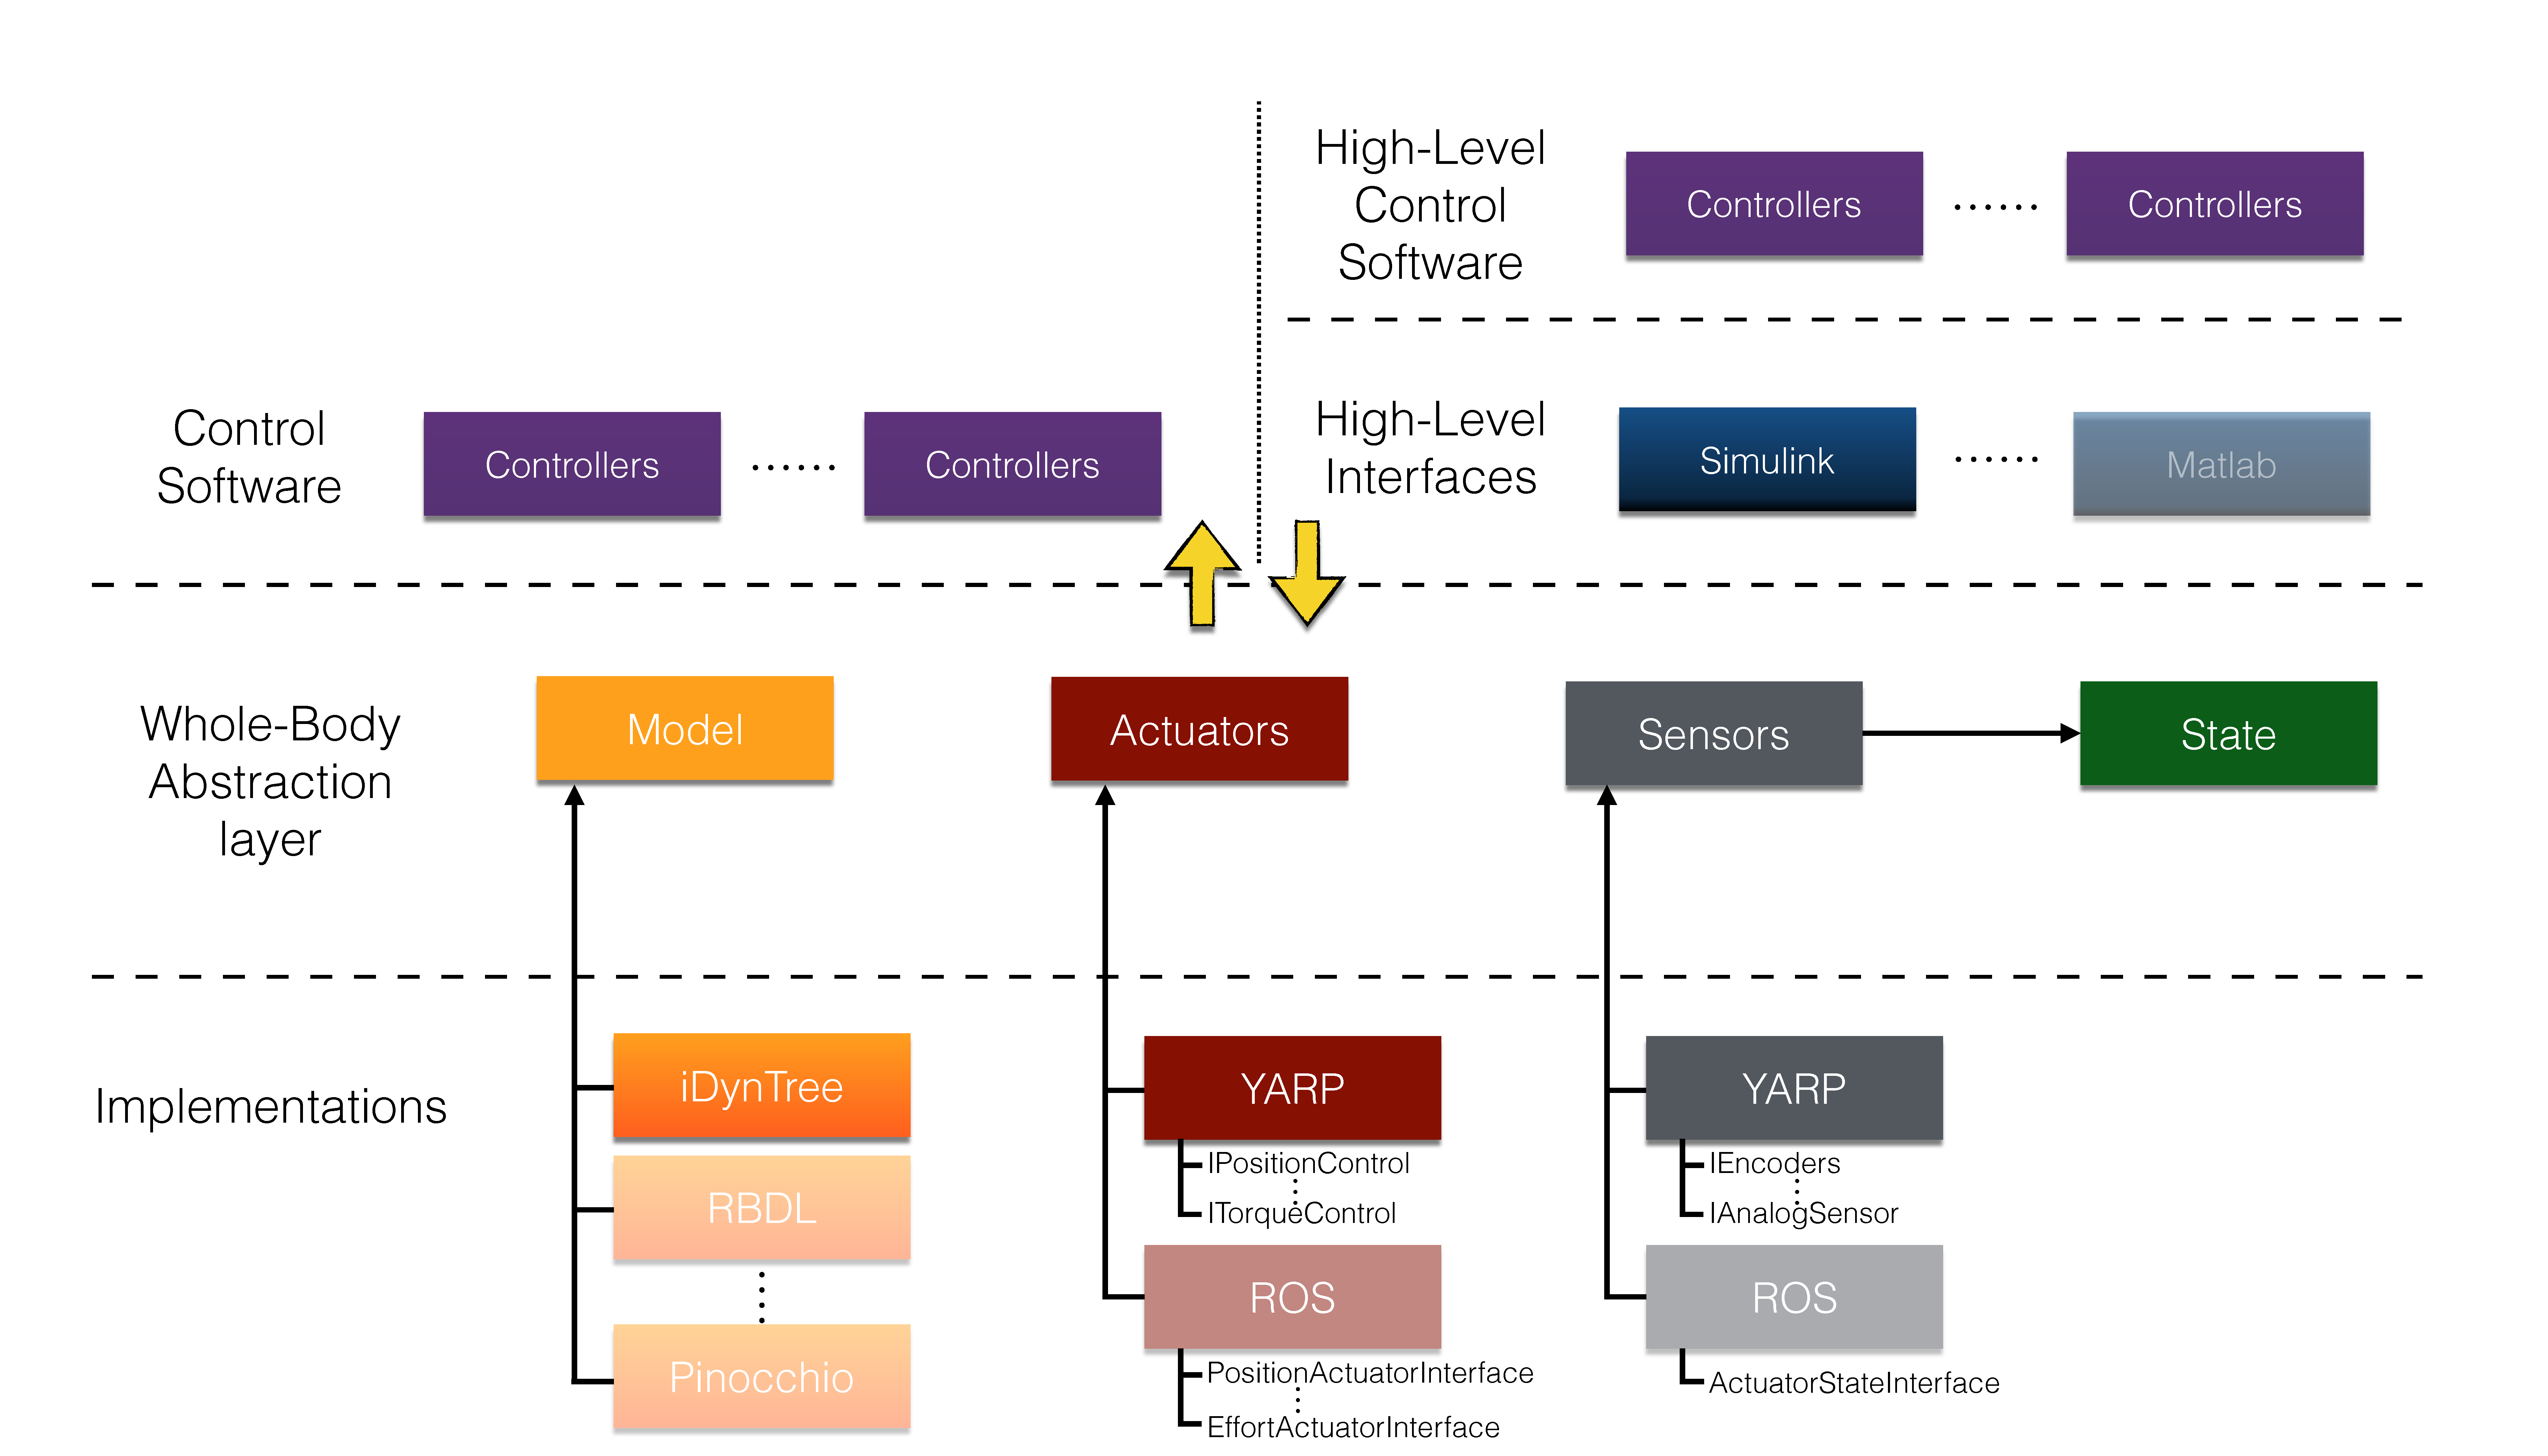
\includegraphics[width=.9\textwidth]{images/WBI_diagram.pdf}
  \caption{Whole-body Interface software architecture}
  \label{fig:images_WBI_diagram}
\end{figure}
%

%% \paragraph{Related Publications:}
%% \begin{itemize}
%%     \item \bibentry{romano2017whole}
%% \end{itemize}


\subparagraph*{System dynamics estimation software. Extension to
environmental compliance estimation (T1.4)}

The goal of T1.4 was to include compliant contact estimation to the software.
This is part of \texttt{codyco-superbuild} software which its details are
reported in deliverables D1.1, D1.2 and D1.3.


\subparagraph*{Extension and enhancement of the iDyn library. (T1.5)}

As part of this task, INRIA developed several software modules which are all
available on github.  These modules which have been used as a support for the
research in the other WPs are:
\begin{itemize}
  \item software and GUI for visualizing the whole-body torques of iCub:
    \url{https://github.com/inria-larsen/icub-wholebody-visualization}
  \item software for interfacing the Geomagic software with Gazebo and use it
    for haptic interaction with iCub:
    \url{https://github.com/inria-larsen/geomagic_touch}
  \item software for learning prioritized controllers, in Matlab, with
    implementation of constrained stochastic optimization algorithms:
    \url{https://github.com/serena-ivaldi/learnOptimWBC}
  \item software for learning Probabilistic Movements Primitives from
    trajectories acquired by demonstrations on iCub:
    \url{https://github.com/inria-larsen/icubLearningTrajectories}
\end{itemize}


During the fourth year, IIT extended the iDynTree library, i.e. the new
version of the iDyn library, to support a new probabilistic based estimation
algorithm with redundant measurements, called Bayesian Estimation for Robot
Dynamics, (BERDY).  BERDY algorithm can be used to estimate the dynamics of
any mechanical system by adopting a sensor fusion approach.  Indeed,
information coming from multiple sensors such as IMUs, force/torque sensors,
etc, can be integrated together with their corresponding variance so as to
obtain the probability density function of the estimate of the whole-body
dynamics of the considered system.  When the Gaussian hypothesis is used, the
dynamics estimation can be obtained by solving a linear system of equations,
which are intrinsically sparse.  This led to the implementation in iDynTree of
a compressed row storage (CRS) scheme for sparse matrices.  Preliminary
results seems to report an increment in the computational performance of about
$40\%$with respect to the dense implementation.  To ease the development of
algorithms and batch data processing, the iDynTree library has been extended
to provide support to Matlab scripting.  It is now possible to call iDynTree
functions directly from Matlab scripts.
%
\begin{figure}[h]
  \centering
    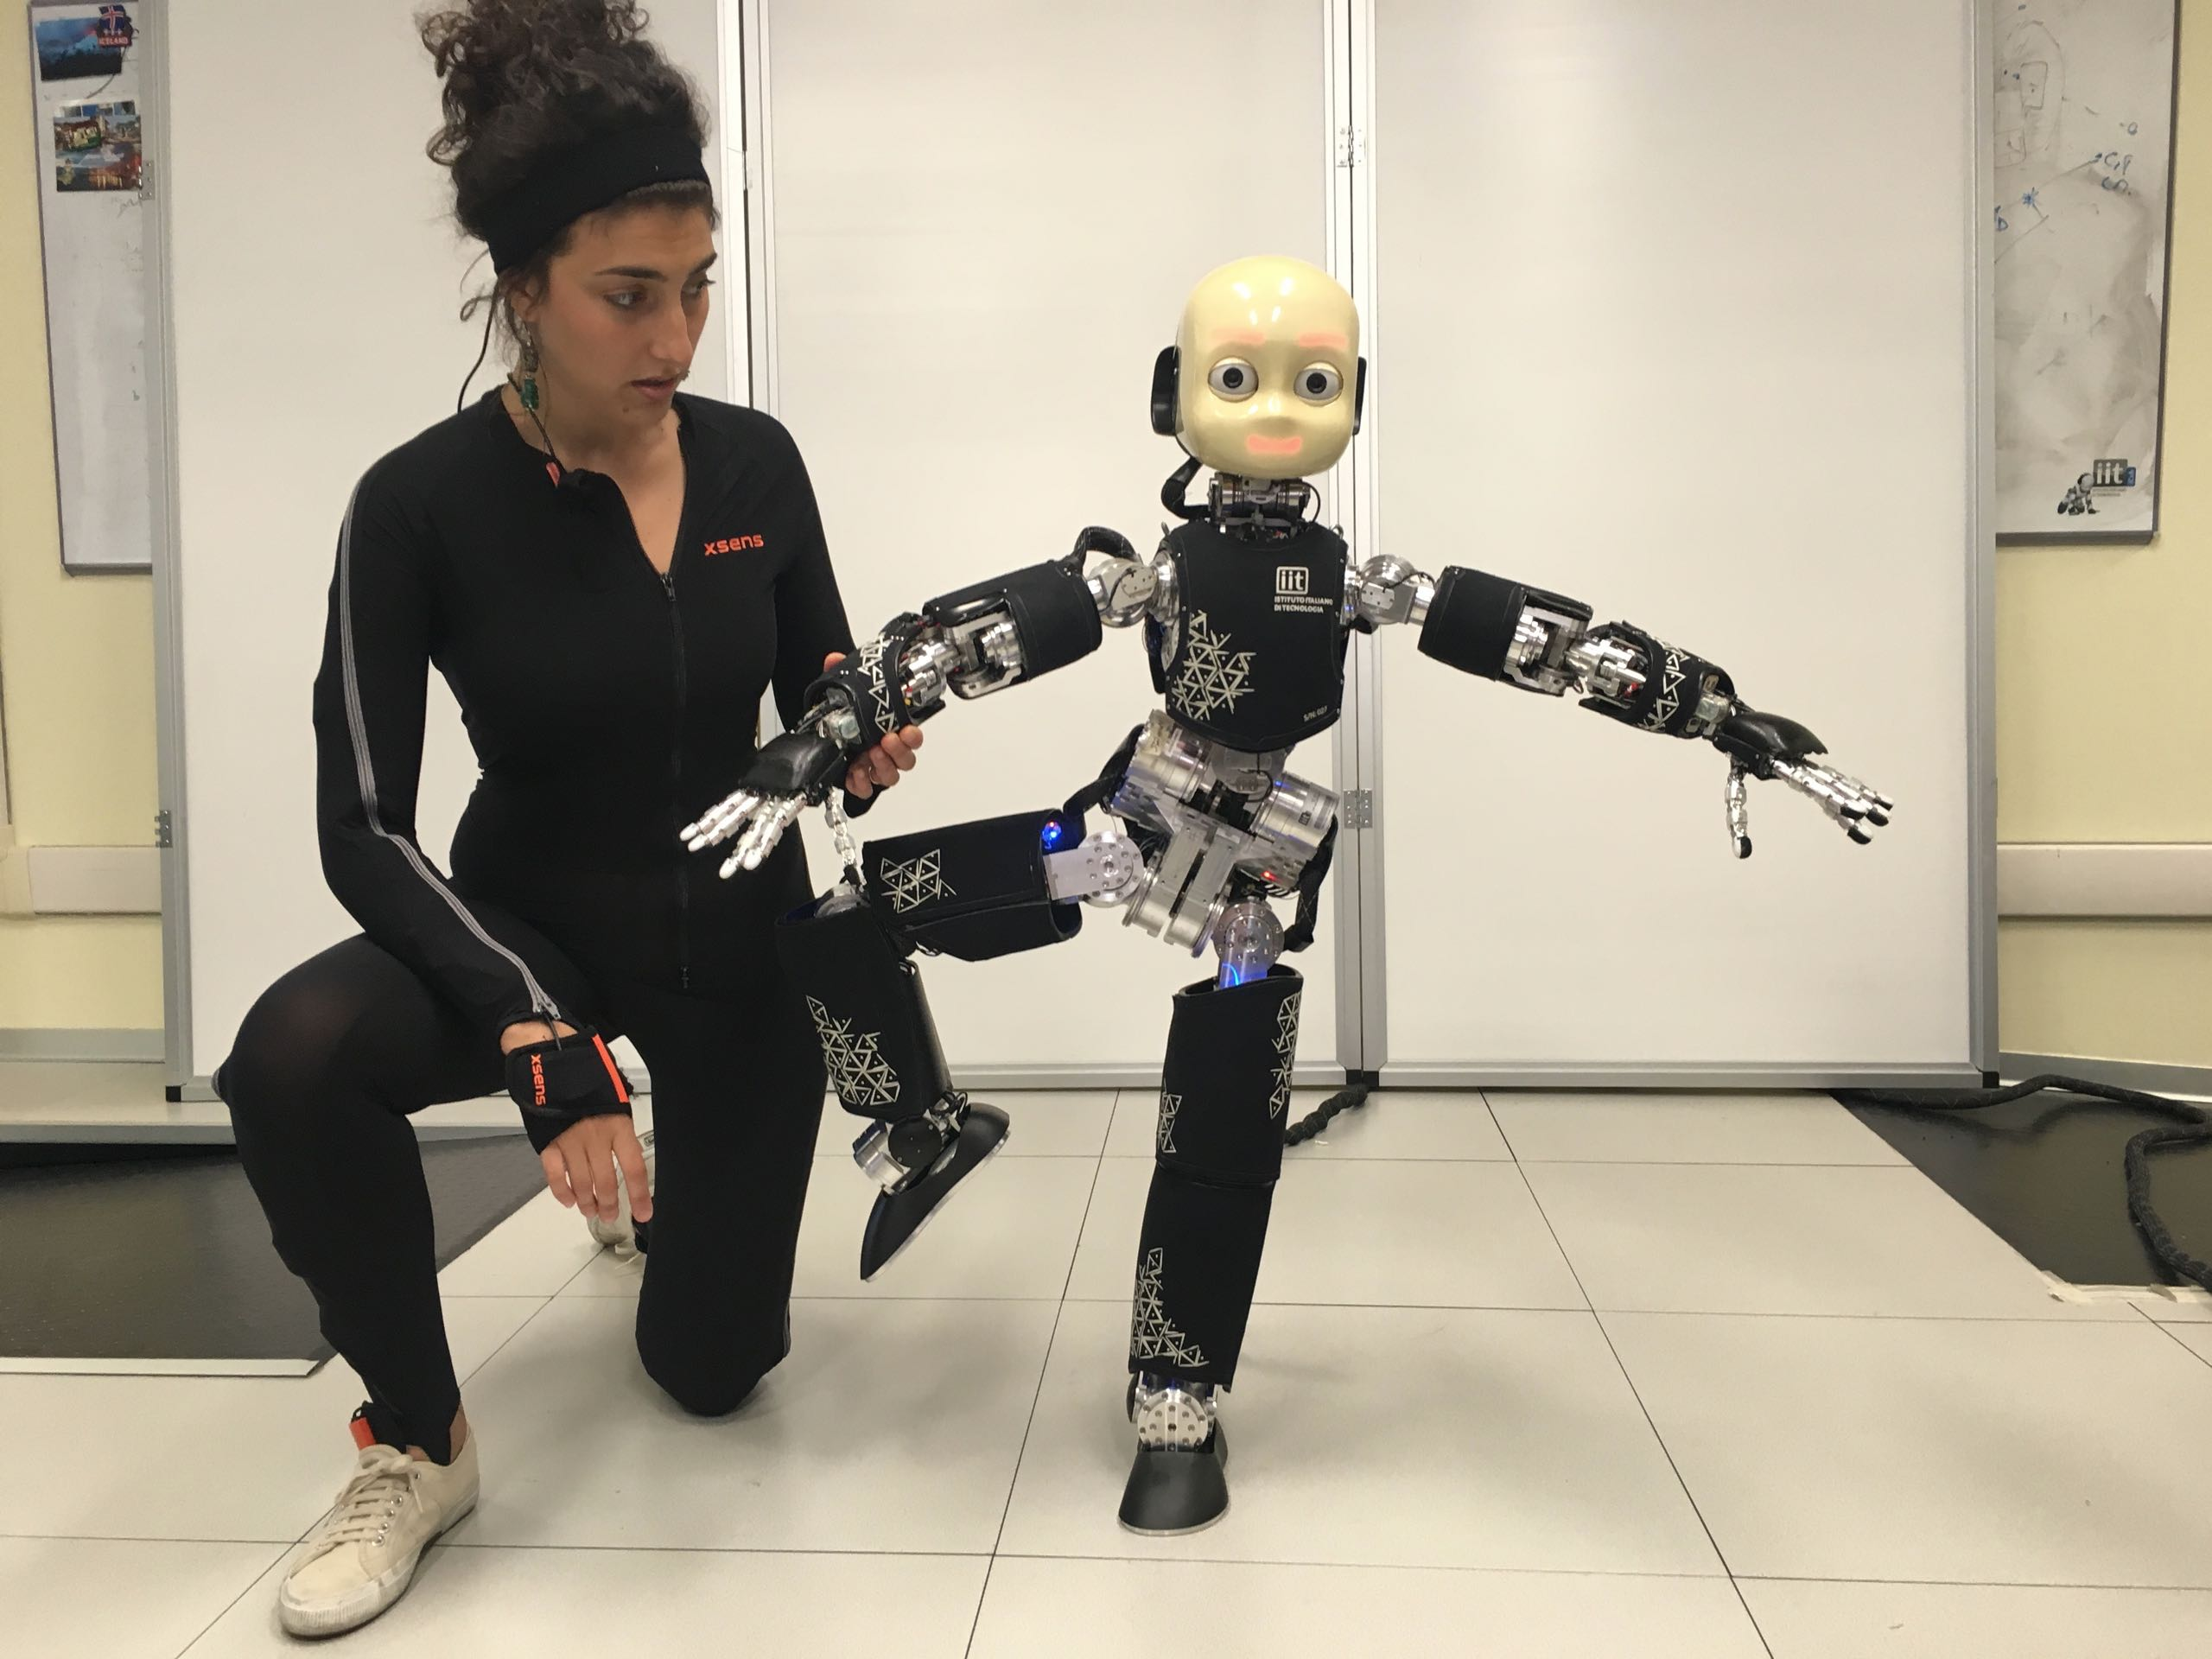
\includegraphics[width=.9\textwidth]{images/suit.jpg}
  \caption{Human interacting with the iCub Robot. The BERDY algorithm can be used to estimate online both the dynamics of the robot and of a human.}
  \label{fig:images_suit}
\end{figure}
%

%% \paragraph{Related Publications:}
%% \begin{itemize}
%%     \item \bibentry{latella2016whole}
%%     \item \bibentry{nori2015simultaneous}
%% \end{itemize}


%!TEX root = ../../thirdYearReport.tex


\subparagraph*{Resources}
Overall, the use of resources within WP1 was in accordance to the plans. 

\begin{center}
  \begin{tabular}{|C{1.5cm}|C{1.5cm}|C{1.5cm}|C{2cm}|C{2cm}|C{2cm}|C{2cm}|}
    \hline \footnotesize \textbf{WP1 person months}& \footnotesize
    \textbf{IIT}&\footnotesize \textbf{TUD}&\footnotesize \textbf{UPMC}&
    \footnotesize \textbf{UB} &\footnotesize \textbf{JSI} & \footnotesize \textbf{INRIA}\\
    \hline \footnotesize Year 1 & 8.67 &1.00 & 3.29 & 0.51 & 2.00 & -\\
    \hline \footnotesize Year 2 & 3.00 & 3.00 & 0.47 & 2.29 & - & - \\
    \hline \footnotesize Year 3 & 5.27 & 1.00 & - & 1.82 & 2.00 & 2.96 \\
    % \hline \footnotesize Partial & 16.94 & 5.00 & 3.76 & 2.8 & 4.00 & -\\ 
	\hline
    \hline \footnotesize Overall & 12.00 & 9.00 & 6.00 & 15.00 & 6.00 & 5.00 \\
    \hline
  \end{tabular}
\end{center}

\subparagraph*{Deviations from workplan} 
No significant deviations. 


%!TEX root = ../../thirdYearReport.tex
\paragraph{Work package 2 progress}

\subparagraph{Shared control method in interaction with compliant environment}
~\par
At JSI we studied mutual learning of human and robot in case of interaction with a compliant environment. A novel method for shared control between the human and the robot was developed to efficiently facilitate the robot skill synthesis for the desired interaction. If the robotic skill is incrementally formed (online) while the physical interaction task is performed/taught by the human demonstrator then the robot has the capacity to generate the control commands for the robot already during the learning stage. However, the human is simultaneously controlling the robot in order to teach it how to perform the given interaction task. Therefore, there can be a conflict between the human commands and commands generated by the currently obtained robotic skill. To solve this issue, an additional method was developed that delegates the control responsibility between the two acting agents in tasks involving interaction with compliant environment.

While shared control is a well-studied subject in case of pure teleoperation \cite{Niemeyer2008}, only few studies exist in human-in-the-loop robot teaching framework. One of our previous studies \cite{Peternel2013} focused on developing a shared control method for teaching humanoid robot of compliant whole-body interaction with unpredictable environment in online manner. The control was shared percentually between human and robot based on the average error between the demonstrated actions and the actions from the robot over entire task space up until the current observation time. The disadvantage of this method is that the human cannot efficiently inspect the performance of the currently learnt robotic skill in specific subspace (or state region) of the interaction task. In addition, percentually shared responsibility between the two agents makes it hard for the human to determine who is responsible for a potentially bad performance of the task.

To solve the above-mentioned drawbacks we developed a new method, where the control between the two agents is shared based on the existence of local models in the specific subspace (or state region) of the task. If no local models within the robotic skill exist for a specific subspace, where the task is currently performed, then the control responsibility is given to the human so that he can perform the task through the robot body and at the same time teach it. If local models within the robotic skill exist for the subspace where the task is currently performed, then the control responsibility is given to the robot so that the human can inspect its performance. In case the observed performance is unsatisfactory, the human can update the robot in that specific region. The advantage of this approach is that the skill inspection/correction can be done online (during the demonstration stage) without the need to stop the setup, as opposed to offline robot learning where the skill can be inspected only after the demonstration stage, and if corrections are required the demonstration stage has to be repeated.

The control was shared between the human and the robot as \cite{Peternel2013}
\begin{equation}
y_{cmd} = C \cdot y_{demo} + (1-C) \cdot y_{robot} ,
\label{eq:delegation}
\end{equation}
where $y_{cmd}$ is a vector of commands sent to the robotic mechanism, $y_{demo}$ is a vector of commands given by the human demonstrator, $y_{robot}$ is a vector of commands produced by the current state of robot and $0 \leq C \leq 1$ is a weight factor that determines the influence of each agent. Pure human control is achieved when $C = 1$, and pure machine control is achieved when $C = 0$.

The practical implementation of the proposed method was done based on Locally Weighted Regression (LWR)\cite{Schaal1998}. LWR is an online machine learning method that approximates the non-linear model of demonstrated skill with a subset of local linear models. Each local linear model is fitted with a receptive field within the state region that determines its domain. The receptive fields are usually realised by a Gaussian kernel functions so that the closer the current input value is to its centre the higher the activation is. In term, higher higher activation of receptive field means higher influence of the corresponding local model on the output prediction. The prediction of output variable $y$ based on some new input variable $x$ is defined by a sum of contribution of all local models, where the models closer to the input variable have higher impact.

In the proposed shared control method the control responsibility between the two agents depends on the activation of the receptive fields of the local models of LWR. If the activation in a given state region is above some predefined threshold $w_{th}$, sufficient local models exist and therefore the control is given to the robot ($C=0$) so that the human can inspect its performance. In opposite case, if activation is below $w_{th}$, no sufficient local models exist and therefore the control is given to the human ($C=1$) to perform an additional teaching. The method can be expressed as:
\begin{equation}
C = \begin{cases} 0 & \quad \text{if } w_{max} > (w_{th} + \frac{d}{2})
\\ \frac{ 1 + \cos \big(\pi \frac{w_{max} - (w_{th} - \frac{d}{2}) }{d}\big)}{2} & \quad \text{if } (w_{th} - \frac{d}{2}) \leq w_{max} \leq (w_{th} + \frac{d}{2})
\\ 1 & \quad \text{if } w_{max} < w_{th} - \frac{d}{2}) \\ \end{cases}
\label{eq:factor}
\end{equation}
where $w_{max}$ is the activation of the model receptive fields \cite{Schaal1998} and $w_{th}$ is an activation threshold that we introduced to determine the model-proximity based shared control. The switching of responsibility between the human and the robot control is essentially binary to provide the human with a clear feedback about who is responsible for the given task performance. However, we implemented a cosine function to prevent sudden jumps between the two states of responsibility, were $d$ defines the width of switching function.

LWR allows incremental update of local models by feeding a new data point [$x$,$y$] each sample time. However, in such case it is hard for human to inspect the robotic skill performance of some subspace of the task as the skill is constantly changing/updating. Therefore we accumulated the training data points for some predefined amount of samples before we fed them to the LWR to update the models:
\begin{equation}
A_{new} = \begin{cases} A & \quad \text{if } C \neq 1
\\ [\thinspace A; \thinspace [x, \thinspace y]\thinspace ] & \quad \text{if } C = 1 \text{ and } length(A) < N_{acc}
\\ [\thinspace] & \quad \text{if } length(A) = N_{acc} \\ \end{cases}
\label{eq:accumulate}
\end{equation}
\begin{equation}
A_{in} = A(randperm(N_{acc}),\thinspace :)
\label{eq:shuffle}
\end{equation}
where $A$ is the training data accumulation buffer and the notation $A_{new}$ indicates that $A$ is updated at each iteration. $N_{acc}$ defines the accumulation length in samples before the new model update is made. Before the data is fed to the LWR the training data in accumulation buffer randomly shuffled in $A_{in}$ buffer.

\begin{figure}[!t]
	\centering
	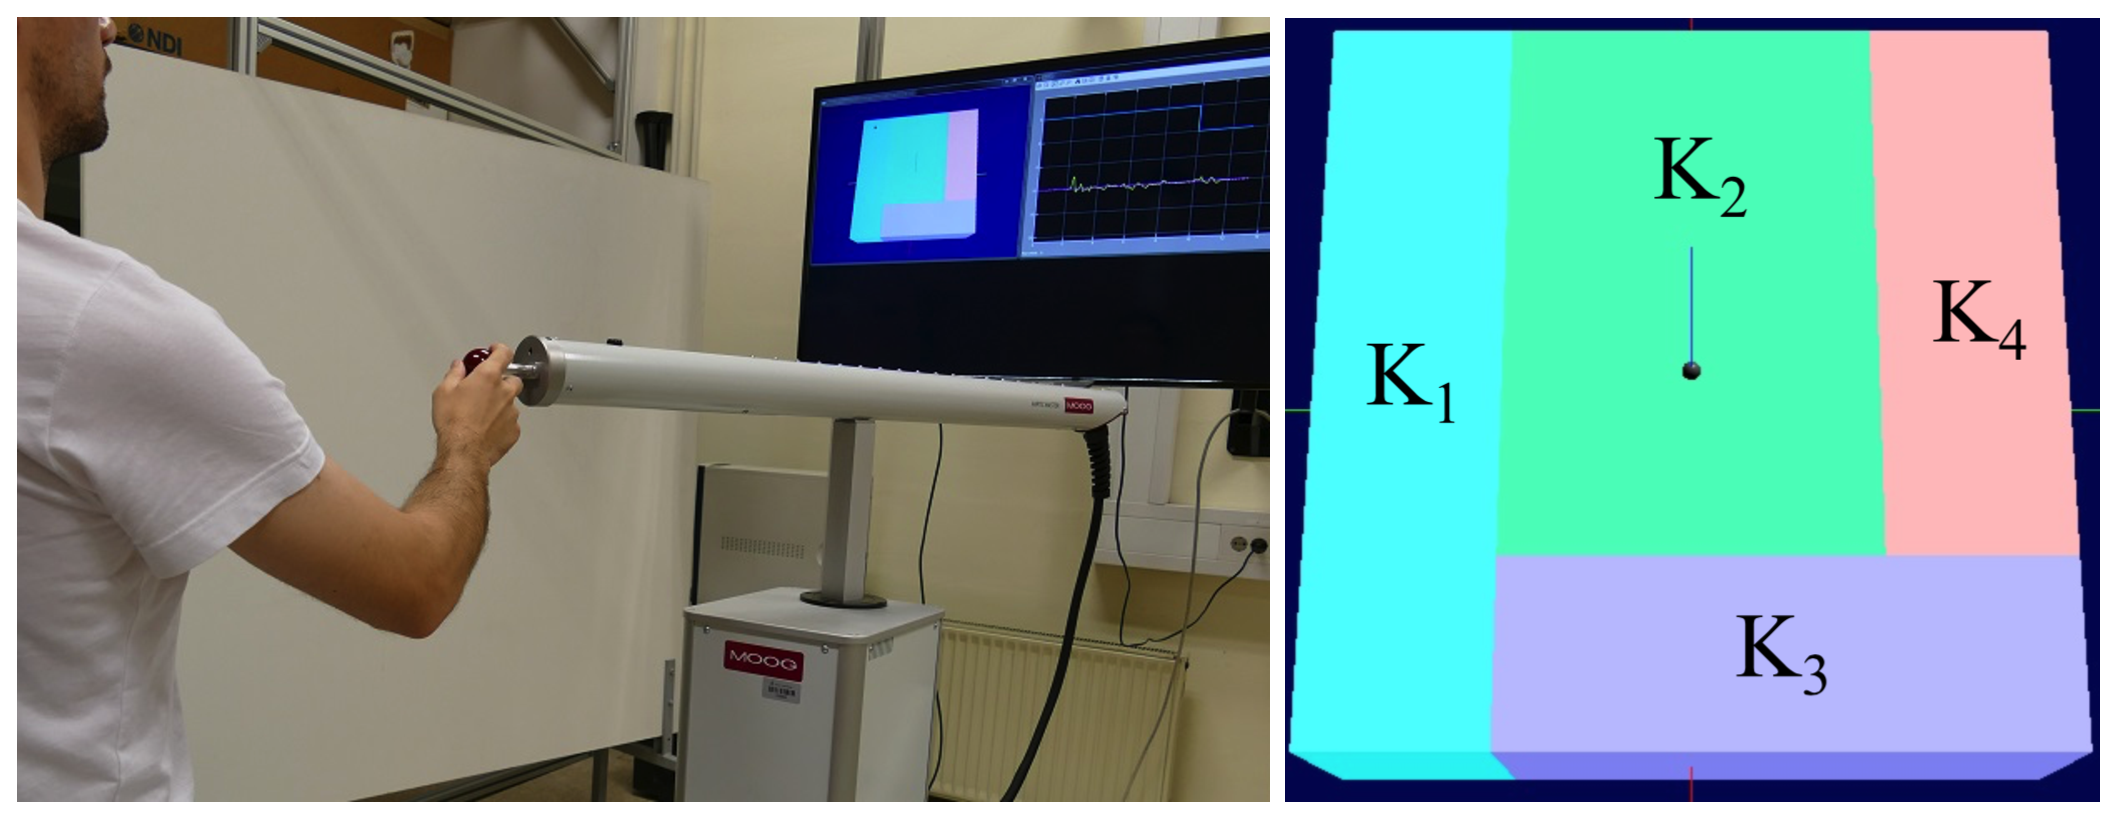
\includegraphics[width=0.99\textwidth]{setup.eps}
	\caption{Robot manipulator control interface consisting of HapticMaster robot and monitor for providing human with visual feedback (right photo). Compliant environment with different stiffness properties (left photo).}
	\label{fig:setup}
\end{figure}

\textbf{Experimental validation:} We validated the proposed method with the experiments on HapticMaster robot \cite{Linde2002}. The experimental setup is shown in Fig. \ref{fig:setup} left photo. The task of the robotic manipulator was to interact with a compliment environment in a way to produce some desired interaction force. The environment and robotic manipulator were simulated. We constructed a 0.4 by 0.4 m object so that its surface was in x-y (horizontal) plane of the reference frame, where different sections had different stiffness properties. See Fig. \ref{fig:setup} right photo for configuration of the object stiffness properties. The parameters were set $k_1=100$ N/m, $k_2=150$ N/m, $k_3=300$ N/m and $k_4=500$ N/m. The robotic manipulator had to produce a desired force $F_z=100$ N along z axis (vertical), which was perpendicular to the object surface. The necessary interaction force control policy was defined as:
\begin{equation}
F_{z} = K(x,y) \big(z_r-z_a\big),\label{en:robotimp}
\end{equation}
where $F_{z}$ is the interaction force acting between the manipulator and the object surface, $K(x,y)$ is the stiffness of the object in z axis, $z_a$ is actual and $z_r$ is reference position of the manipulator's end-effector in z axis. When the manipulator was on the softer section of the object surface (i.e. lower stiffness $K$), the reference position had to be put deeper inside the object to produce the desired force. In opposite case, when the manipulator was on the harder section of the object surface (i.e. higher stiffness $K$), the reference position had to be put closer to the surface to produce the same desired force.

The results of the experiment are shown in Fig. \ref{fig:models}. The top row shows the acquired models (robotic skill) for manipulator's displacement of reference position from the actual position in z axis. Each column represents the different stage of training data update. The time stamps of the update application are displayed on the top. The middle row shows the force prediction error of the obtained models at each stage. The bottom row shows the motion of the robot manipulator (thick black and green line) on the surface of the object (thin black rectangle). The black line shows the trajectory when the demonstrator had the control over the robotic manipulator's force production task. The green line shows the trajectory when the robot had the control over the robotic manipulator's force production task. The red crosses show the centres, while blue ellipses show the threshold activation ranges $w_{th}$ of the currently available local models that are part of robotic skill.

\begin{figure}[!t]
	\centering
	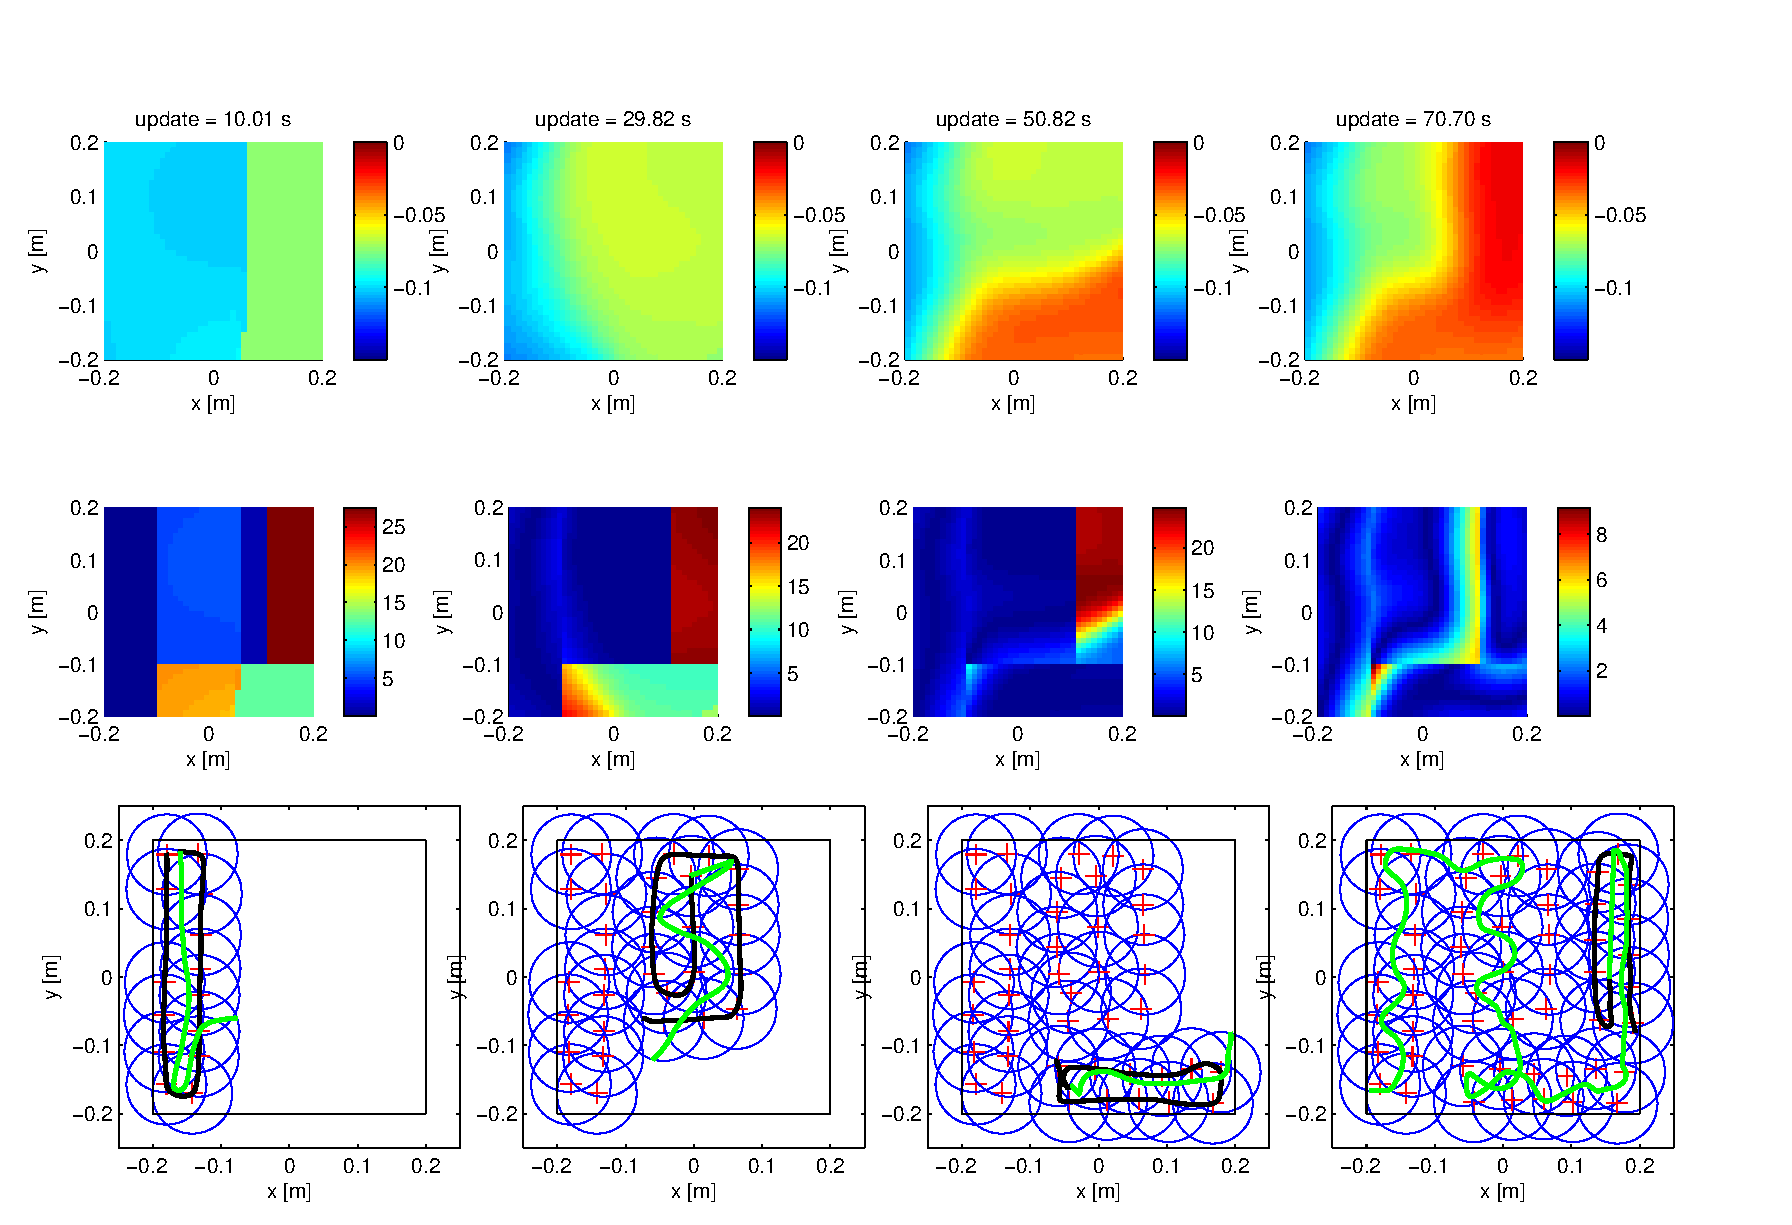
\includegraphics[width=0.99\textwidth]{models.eps}
	\caption{Result of the experiment. Graphs in each column correspond to the stage when the robot was updated. The upper row graphs show the performance of the robot in terms of control of reference position along z axis. The second row shows the error between the reference force and the force produced by the robot. The third row shows the trajectory of motion of robotic manipulator end-effector when the control responsibility was given to human (black line) and when it was given to robot (green line). The influence of local models is shown by blue ellipses and its centres by red crosses.}
	\label{fig:models}
\end{figure}





\subparagraph{Human motor control learning during compliant interaction with environment}

In this study performed at UB we aimed to examine how humans learn compliant force dynamics and modulate their whole-body motions to reach anticipated goals. Here, we present an experimental idea to measure the goal-directed movements against compliant forces, and then illustrate the ongoing results which were conducted for a few human subjects. At this pilot stage, we are focusing on the simple linear compliant case and discuss further experiments. To deepen understanding of the mechanism in humans, it would be beneficial to develop the humanoid robot control in interacting with multiple compliant surfaces.

%%%%%%%%%%%%%%%%%%%%%%%%%%%%%%%%%%%%%%%%%%%%%%%%%%%%%%%%%%%%%%%%%%%%%%%%%%%%%%%%
%\section{Introduction}

\textbf{Introduction:} Humans can learn how to control their own body movements in an uncertain environment, and utilise it to predict the consequences of actions and to achieve a behavioural goal \cite{Wolpert11, Davidson&Wolpert03}. A considerable amount of research has shown the human capabilities of generalization in visuomotor learning and has been exploring the underlying mechanisms \cite{Goodbody&Wolpert98, Krakauer06}. A certain exposure to a new physical environment facilitates to generalize the spatial and temporal characteristics of the point-to-point movements via error-based learning and perturbation paradigm. In the real-world interactions, there are varied and complicated force dynamics (i.e., governed by not only simple linear principles) when making a contact with an object and handling it. The optimal functions seem to be perceptually learned via repetitive movements against the force. However, to our knowledge, little is still known about how humans can generalize the compliant force dynamics itself and utilize it to their future motor plan.

The CoDyCo project has been investigating the whole-body coordination mechanisms in arm reaching movements and the postural balance control in assistive contact with rigid and/or compliant surfaces. Like humans, robots are required to flexibly adjust their posture and to coordinate the physical mobility with augmented autonomy. We expect that humans could generalize the force principles in a cognitively robust way via force-feedback from the early stage of the body movements. To explore the generalization mechanism of the force dynamics in humans and to model it would provide a useful strategy in humanoid robot control. The successful model could be exploited to effectively control autonomous robots' whole-body balance in interacting with the environment through supportive contacts.

In a pilot study, we focused on a simple case: linear compliant force. We employed a haptic device, Haptic Master (Moog, Inc.), which is controlled by a set of a computer programmes to render robotic manipulandum for force feedback. The pilot experiment measured the end-effector movements controlled by human subjects and analysed the dynamic properties of the movements against the compliant force and the performance.


%%%%%%%%%%%%%%%%%%%%%%%%%%%%%%%%%%%%%%%%%%%%%%%%%%%%%%%%%%%%%%%%%%%%%%%%%%%%%%%%
%\section{Methods}

%\subsection{Modelling}

\textbf{Modelling:} In general, spring-damper force ($\BF$) is formulated by the position and the velocity with parameters: spring stiffness ($k$) and spring damping factor ($\lambda$). Here, it is simplified for one direction ($\BZ$).
%
\begin{equation}
\BF = k \BZ^n + (\lambda \BZ^p) \dot{\BZ} \, .
\end{equation}
%

We employed the ready-made spring model in the Haptic API, where the compliant force formula was assigned to the device, the Haptic Master. The compliant force was rendered by the end-effector position and the velocity with the parameters in real-time (Fig. \ref{modelling}). 
%
\begin{figure}
	\centering
	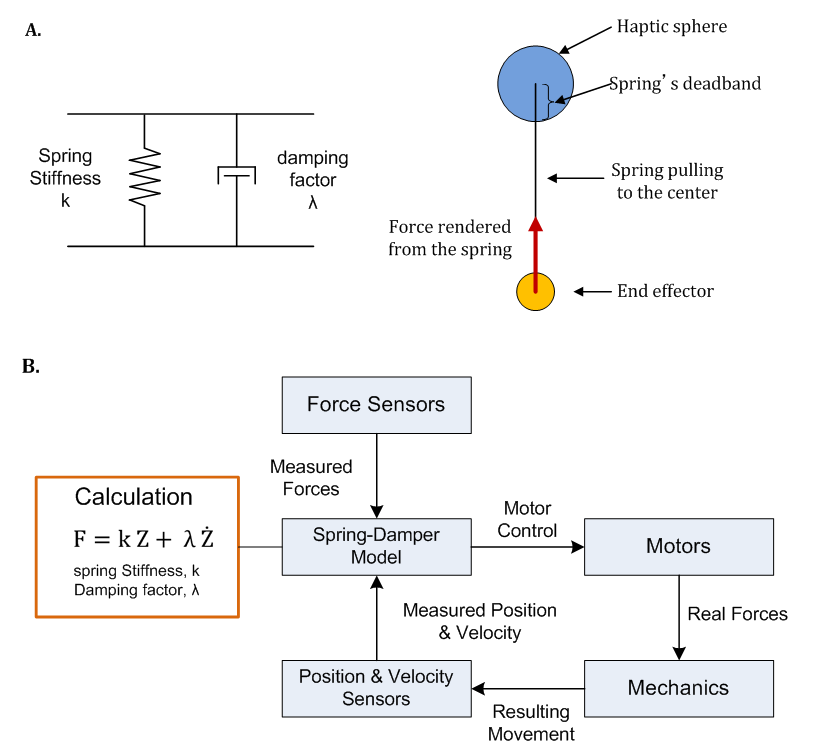
\includegraphics[scale=0.5]{fig1.png}
	\caption{A. The ready-made spring model in the Haptic API. B. Block diagram of the compliant force control. The force is rendering based on the end-effector position and the velocity with parameters (spring stiffness and damping factors) in the real time.}
	\label{modelling}
\end{figure}


%\subsection{Experimental Design}

\textbf{Experimental design:} As a pilot study, we employed a simple linear spring-damper formula:
%
\begin{equation}
\BF = k \BZ + \lambda \dot{\BZ} \, .
\end{equation}
%
The compliant force formula is assigned to the model in the Haptic Master. Aiming to simplify analysing the performance, the forces and the movements were constrained in the only one direction, here, in the vertical
(Z) direction to the ground.

Human subjects learned a spring compliant force via repetitive reaching movements to the first target ($z = t_1$) in a certain period of time, - so called ``Learning session''. Then, they were asked to move the end-effector to the second, or test, target ($z = t_2$), which was set more far from the t1 position, as a test trial; so, more force would be required for this movement (Fig. \ref*{design}). In order to achieve the $t_2$ target, the participants would exploit their prior knowledge of the force dynamics experienced via learning session. We will evaluate whether and how the motion performance is likely to follow the formula previously learned.
%
\begin{figure}
	\centering
	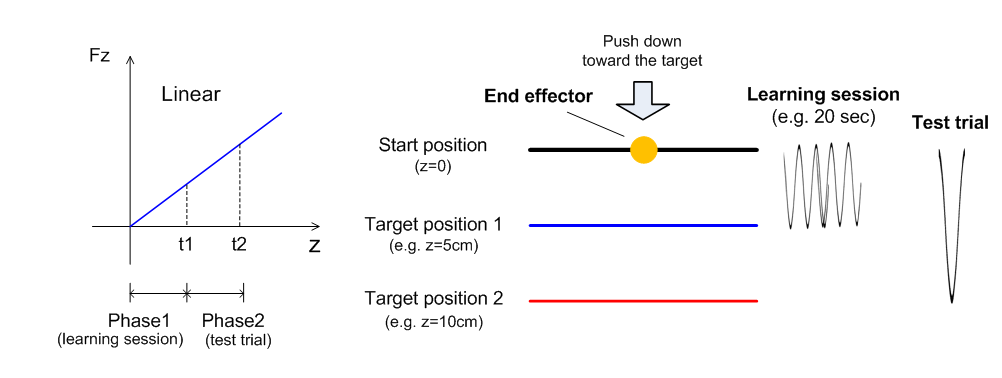
\includegraphics[scale=0.4]{fig2.png}
	\caption{Experimental Design. Two target positions were set: $z = t_1$ for learning session and $z = t_2$ for test trial.}
	\label{design}
\end{figure}


%\subsection{Apparatus and Stimuli}

\textbf{Apparatus and Stimuli:} The haptic device, ``Haptic Master'' consisted of a large robotic rod with an end-effector. The ``Home'' position, where was the centre of the end effector is $z = 0$ at the workspace, was 110 cm from the ground. The spring position was set at $z = 0$. In this study, the rod movements were restricted in the vertical direction only.

The visual information about the task was provided at the computer display to human subjects. The computer screen was located at the right side of the Haptic Master from the subjects; where the centre of the screen was approximately 80 cm from the centre of the robotic rod. The screen was approximately 1 m away from the participants' standpoint, and 80 cm away from the centre of the end effector position. The screen displayed the target position and the end-effector position in real-time (Fig. \ref{stimuli}). The target positions were set at $z = t_1$ (50 mm for learning), and $z = t_2$ (100 mm for test).
%
\begin{figure}
	\centering
	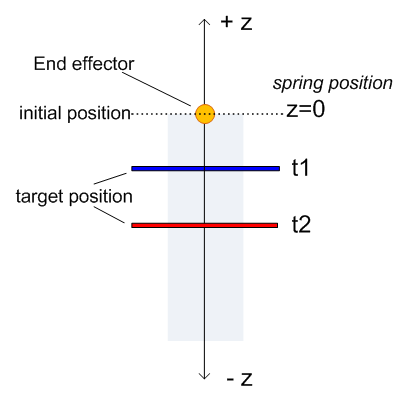
\includegraphics[scale=0.4]{fig3.png}
	\caption{Experimental visual stimuli. The end-effector and the two target positions ($z = t_1$ and $z = t_2$) were visually indicated on the computer screen.}
	\label{stimuli}
\end{figure}

%\subsection{Participants}

\textbf{Participants:} Six male subjects (age: 28.8 +/- 3.1 (SD), height: 175.3 cm +/- 7.1 (SD), weight: 79.5 kg +/- 17.8 (SD), one left-handed) voluntarily participated in the pilot experiment. All had normal or corrected to normal vision, and they had no known motor deficits and/or any limb injuries (self-reported). They were recruited from the student and staff population at University of Birmingham. (One was not naïve to the purpose of the experiment.)

%\subsection{Procedure and analyses}

\textbf{Procedure and analyses:} Participants stood in front of the haptic device and grasped the end-effector. Firstly, they conducted a practice session followed by the main blocks. They were required to make repetitive movements against compliant force generated by the device to learn the kinetic principle. The movements were monitored by visual information on the screen. Participants pushed the end-effector to reach the target position, and then released the end-effector to allow it to freely return to the initial position (z=0). They were asked to set the centre of the end-effector position on the target as accurate as possible. 

The main block consisted of two parts: Learning session and Test trial. In the Learning session, the target position was set at $z= t_1$, described above. Participants controlled the end-effector by their own timing, or rhythm, per each movement in the current pilot study (the specific time windows were not set up by the programme for the series of movements: i.e., push the end-effector down from the start position and reach the target position). The visual feedback was given when the end-effector reached to the target; the target colour indicated this by changing from blue to yellow. Participants learnt the compliant force dynamics by the repetitive movements. he experimenter monitored the elapsed time using a stopwatch, and verbally informed the end of the session when 20 seconds passed. Participant stopped their repetitive movements immediately and prepared for the trial session. 

In the Test trial, participants moved the end-effector to the target (coloured red line, $z = t_2$) three times based on the formula they previously learned. In this phase, no visual feedback in the relationship between the end-effector position and the target was given to the subjects.

One block consists of three sets (Learning session + Test trial). Participants conducted three blocks; so, 3 blocks in total, and 9 test trials. Under the current settings, the experiment was completed within approximately 20 minutes on average.

The dynamic properties of the point-to-point movements were measured: the end-effector's position ($\BZ$), the velocity ($\dot{\BZ}$), and the force ($\BF_Z$) across the time. These were recorded by the 20 msec sampling rate and the properties were analysed and compared between the linear and the non-linear force conditions.

%%%%%%%%%%%%%%%%%%%%%%%%%%%%%%%%%%%%%%%%%%%%%%%%%%%%%%%%%%%%%%%%%%%%%%%%%%%%%%%%
%\section{Results and Discussions}




%\subsection{Ongoing Results}

\textbf{Results:} The end-effector position, velocity and force were recorded. Here, illustrates the one participant's one block performance, as an example (Fig. \ref{results_1}).

In order to examine the each reaching movement, the data were extracted from the total between the start ($z = 0.01 m$) and the end (approx. $z = t_2$) positions, where the end-effector was released to return to the initial position. These points were determined by calculating the each inflection point (Fig. \ref{results_2}).

The data were averaged across three blocks; one block consisted of three (Learning + Trial) sessions; so participants ideally completed 9 sessions in total, but one (subj.03) accidentally completed only two blocks because of the setting errors. The averaged numbers of repetitions were 152.8 +/- 45.6 (SD) in the Learning session and 27.2 +/- 6.1 (SD) in the Test trial. All six participants' averaged data (the end-effector position, velocity and force) can be seen from Fig. \ref{results_3} to Fig. \ref{results_5}.
%
\begin{figure}
	\centering
	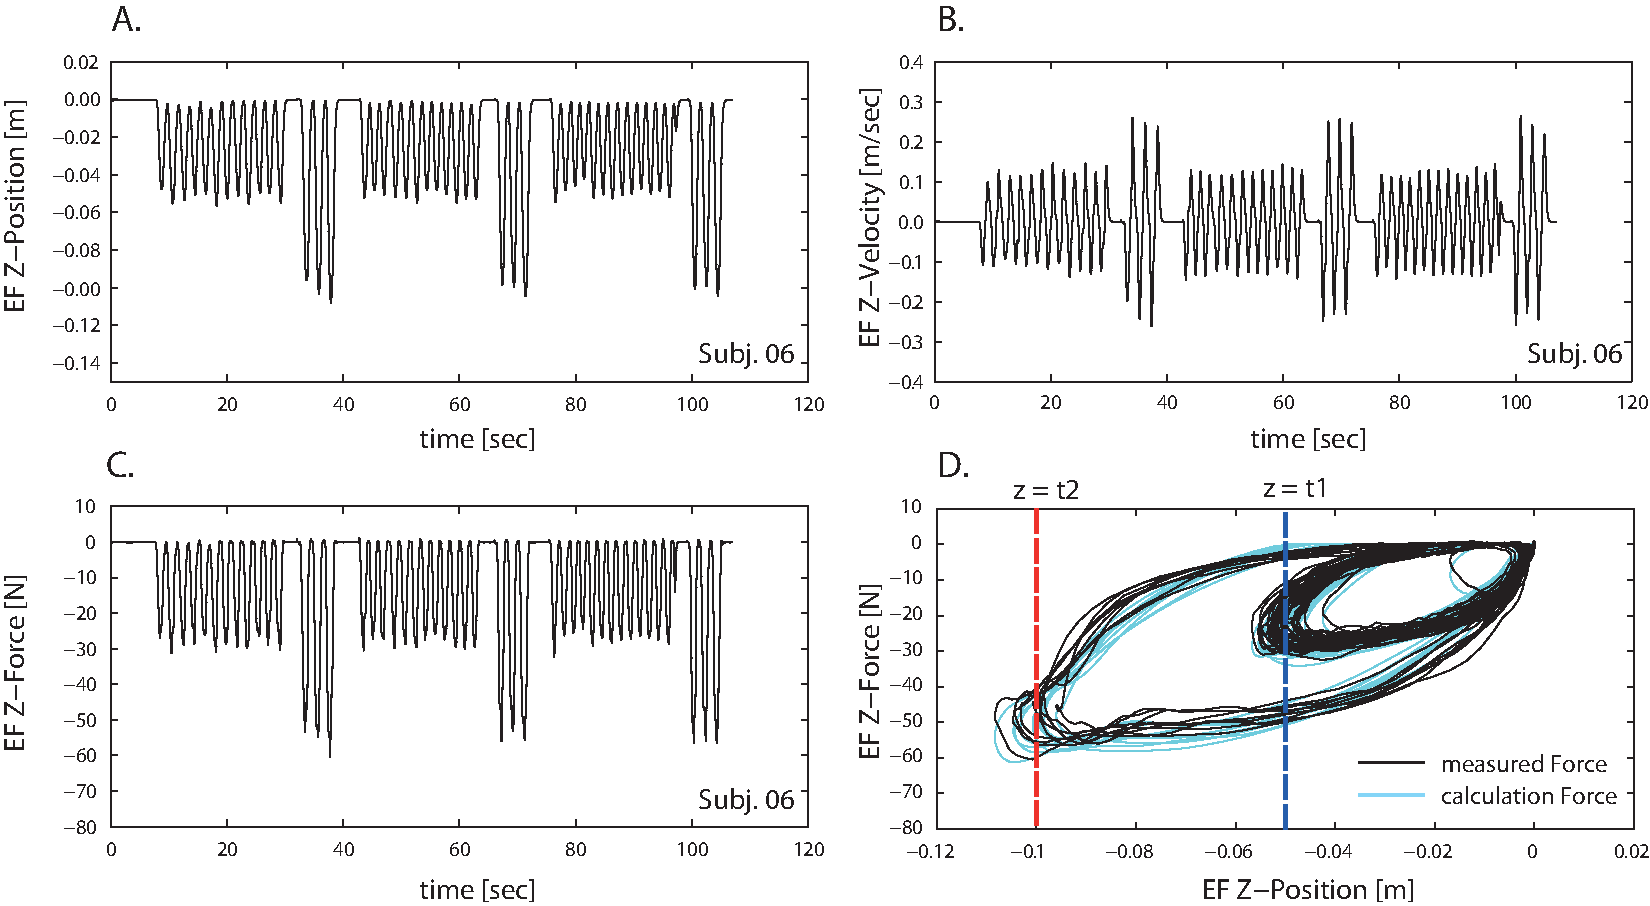
\includegraphics[scale=0.55]{fig4.pdf}
	\caption{The total recording of the completion of the first block. (Subj. 06). $\BA$. End-effector Z-position, $\BB$. Z-velocity and $\BC$. Z-force. $\BD$. the relationship between the position and the force compared between the force directly measured by the sensor and the force calculated by the equation with the real time z-position and z-velocity.}
	\label{results_1}
\end{figure}
%
\begin{figure}
	\centering
	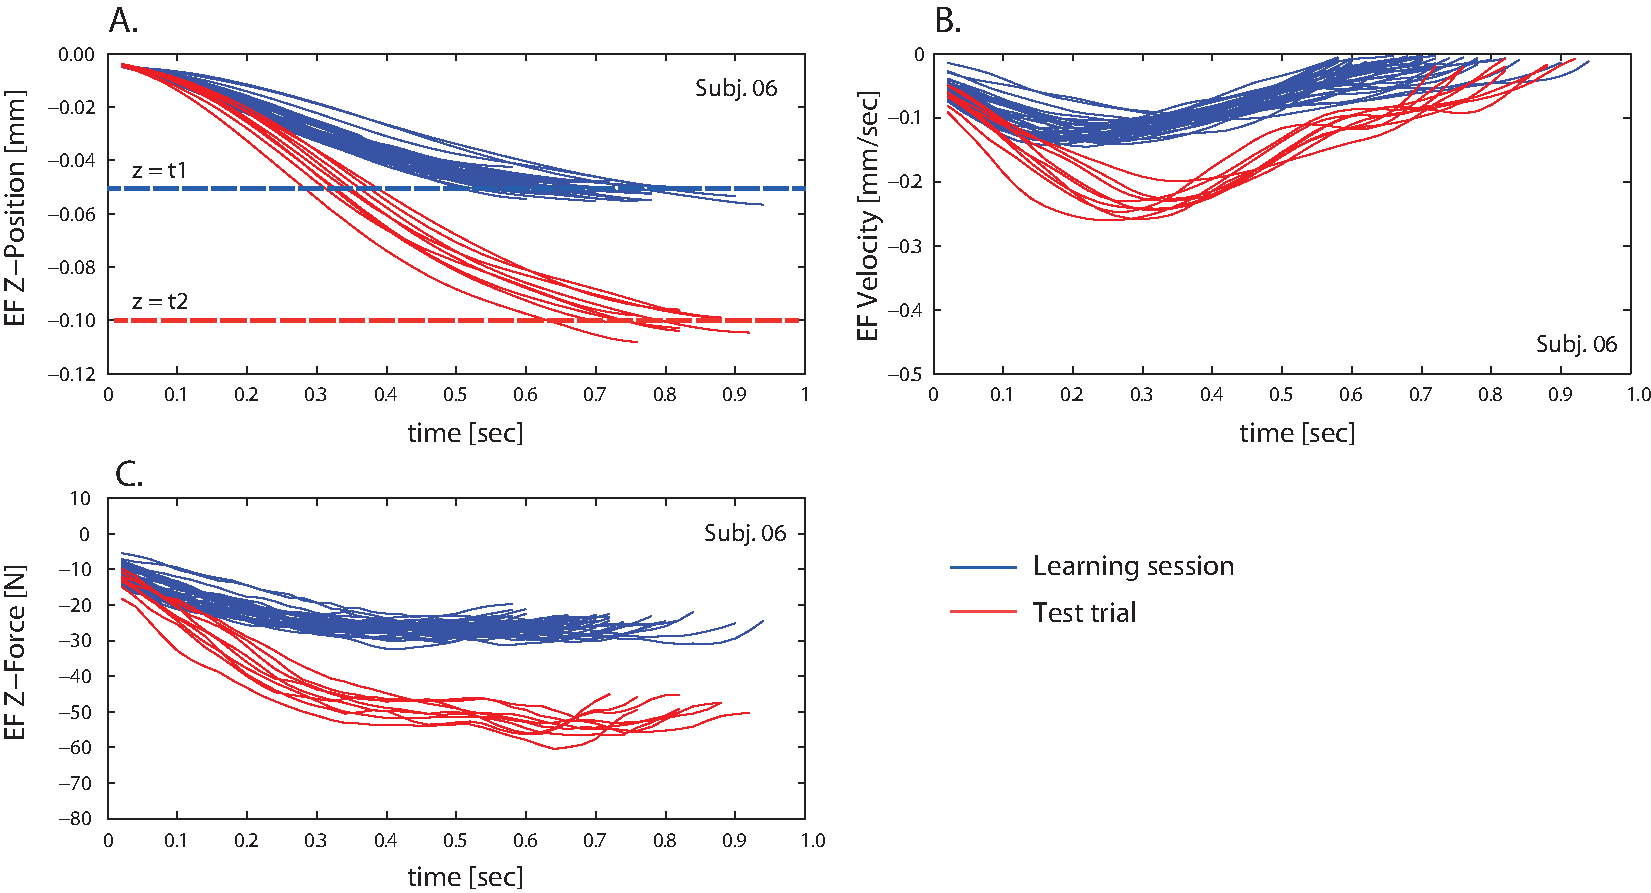
\includegraphics[scale=0.55]{fig5.pdf}
	\caption{Experimental data for one participant (the first block, three test trials). Red lines represent the forces, which were directly measured by a sensor at the end-effector. Blue lines represent the forces, which were calculated in the real time by spring stiffness and damping factor with the end-effector position.}
	\label{results_2}
\end{figure}
%
\begin{figure}
	\centering
	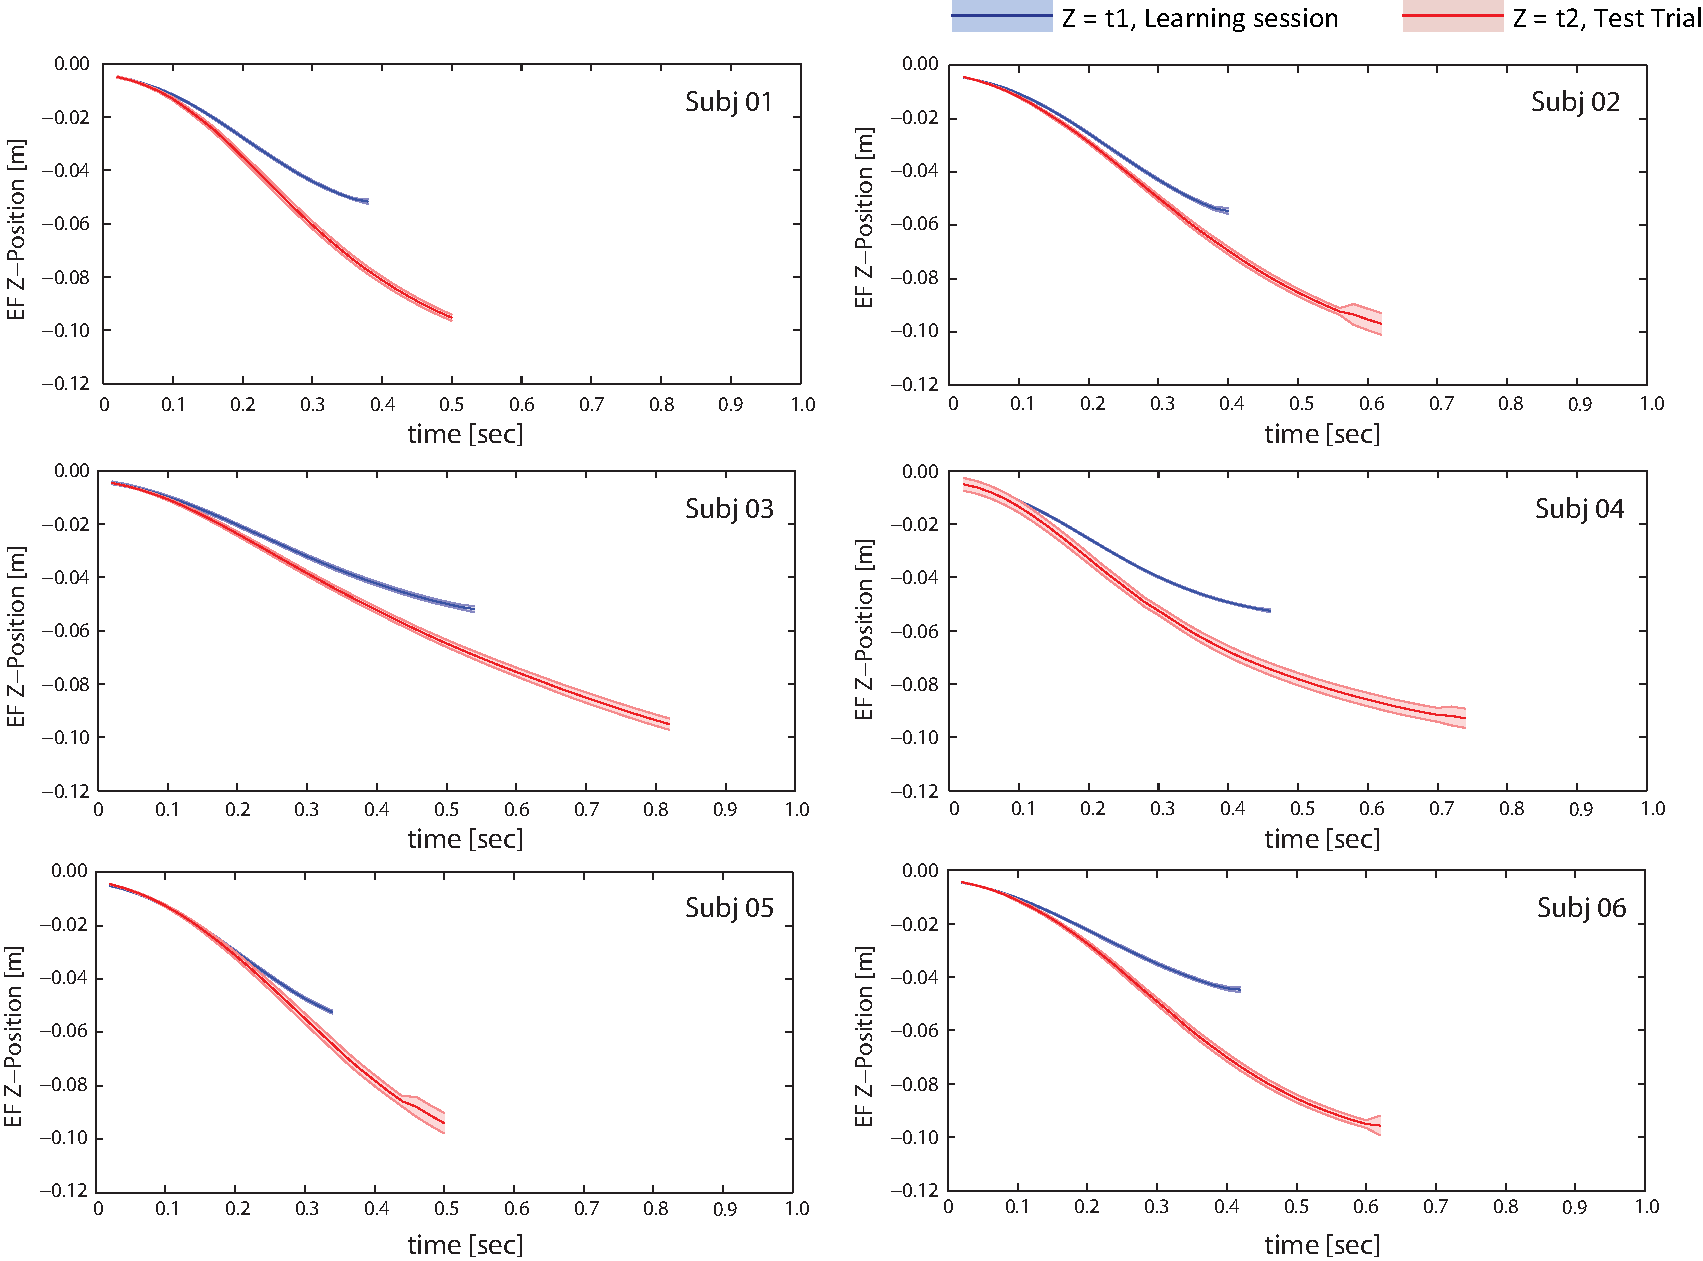
\includegraphics[scale=0.55]{fig6.pdf}
	\caption{The averaged end-effector z-position performance in the reaching movements against the linear spring-damper force for 6 subjects. The data were averaged across 3 blocks (9 (Learning + Trial) sessions). The blue lines represent the average performance in the Learning session, and the red in the Test trial, the coloured areas represent their standard error respectively.}
	\label{results_3}
\end{figure}

\begin{figure}
	\centering
	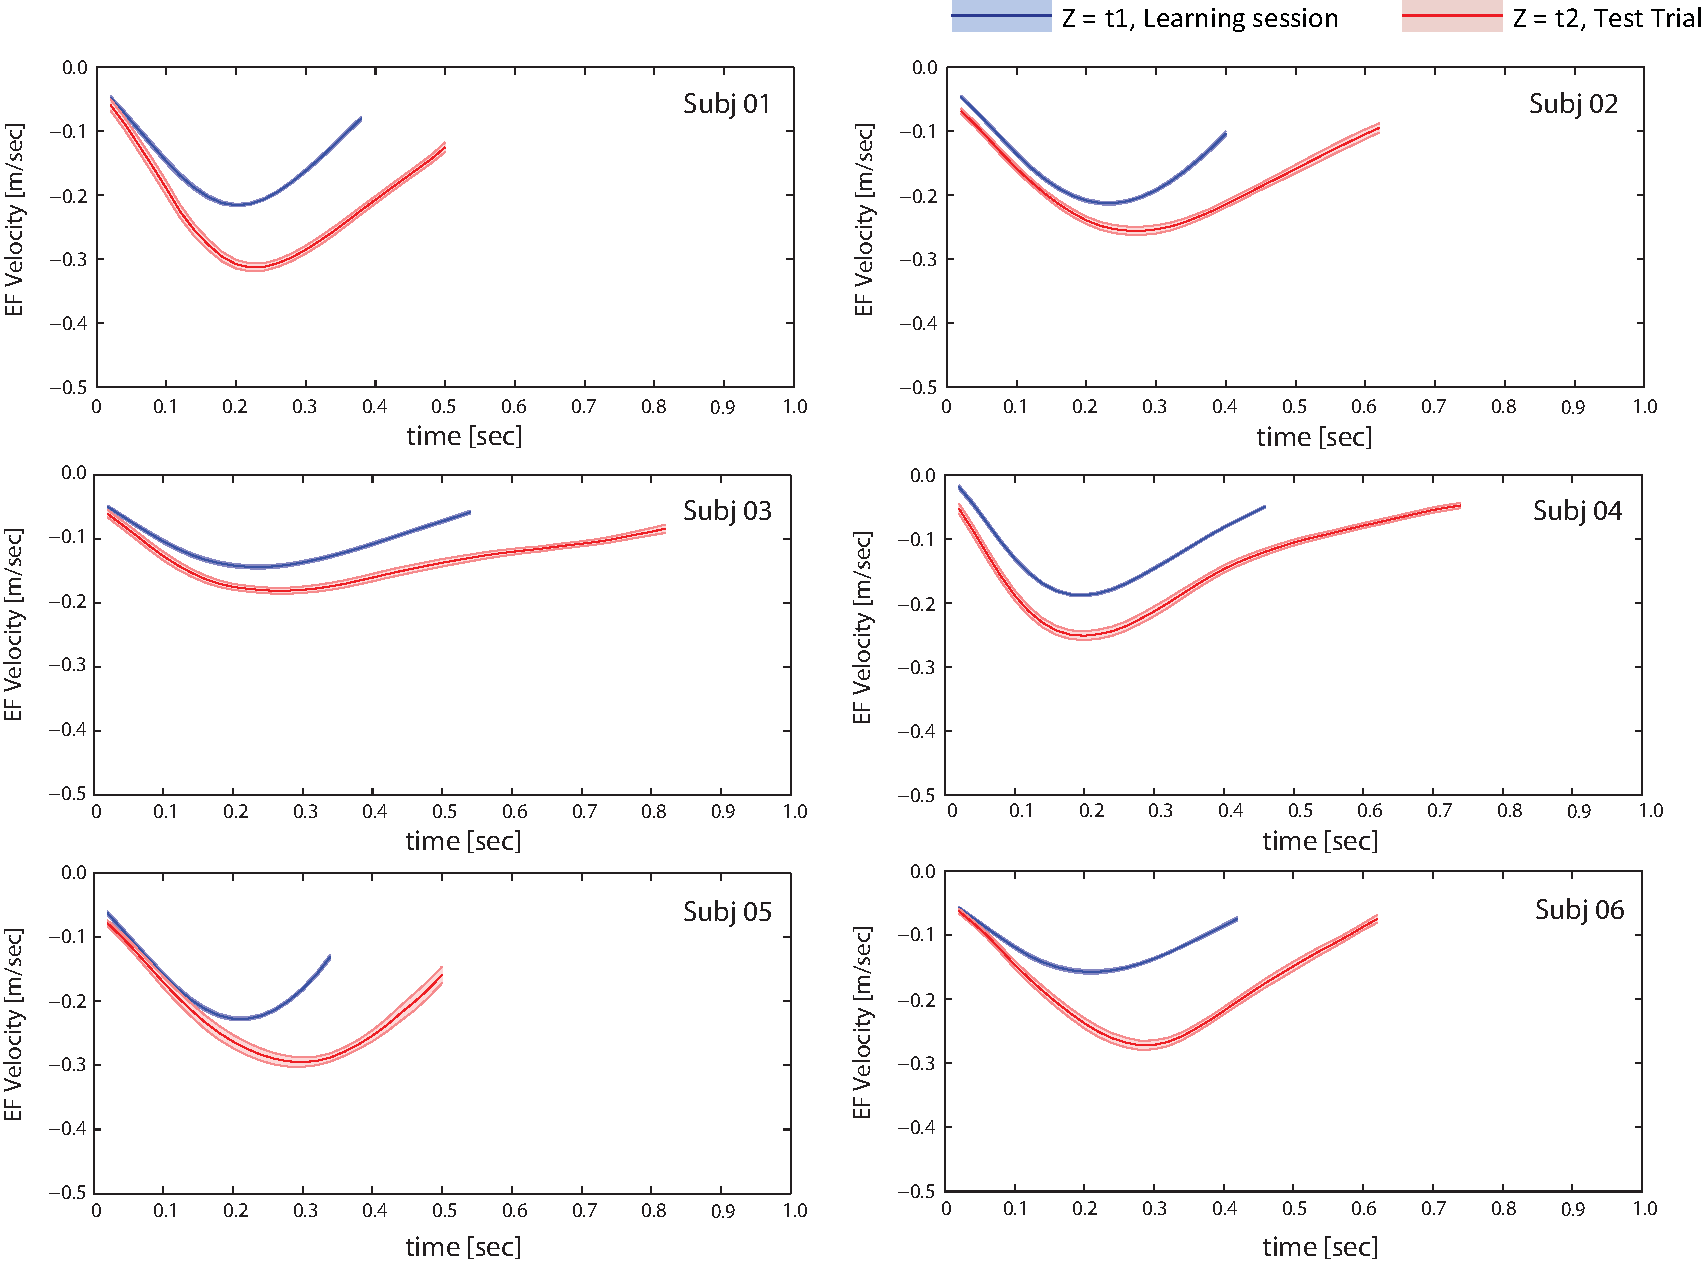
\includegraphics[scale=0.55]{fig7.pdf}
	\caption{The averaged end-effector z-velocity performance in the reaching movements against the linear spring-damper force for 6 subjects. The data were averaged across 3 blocks (9 (Learning + Trial) sessions). 
		The blue lines represent the average performance in the Learning session, and the red in the Test trial, the coloured areas represent their standard error respectively.}
	\label{results_4}
\end{figure}

\begin{figure}
	\centering
	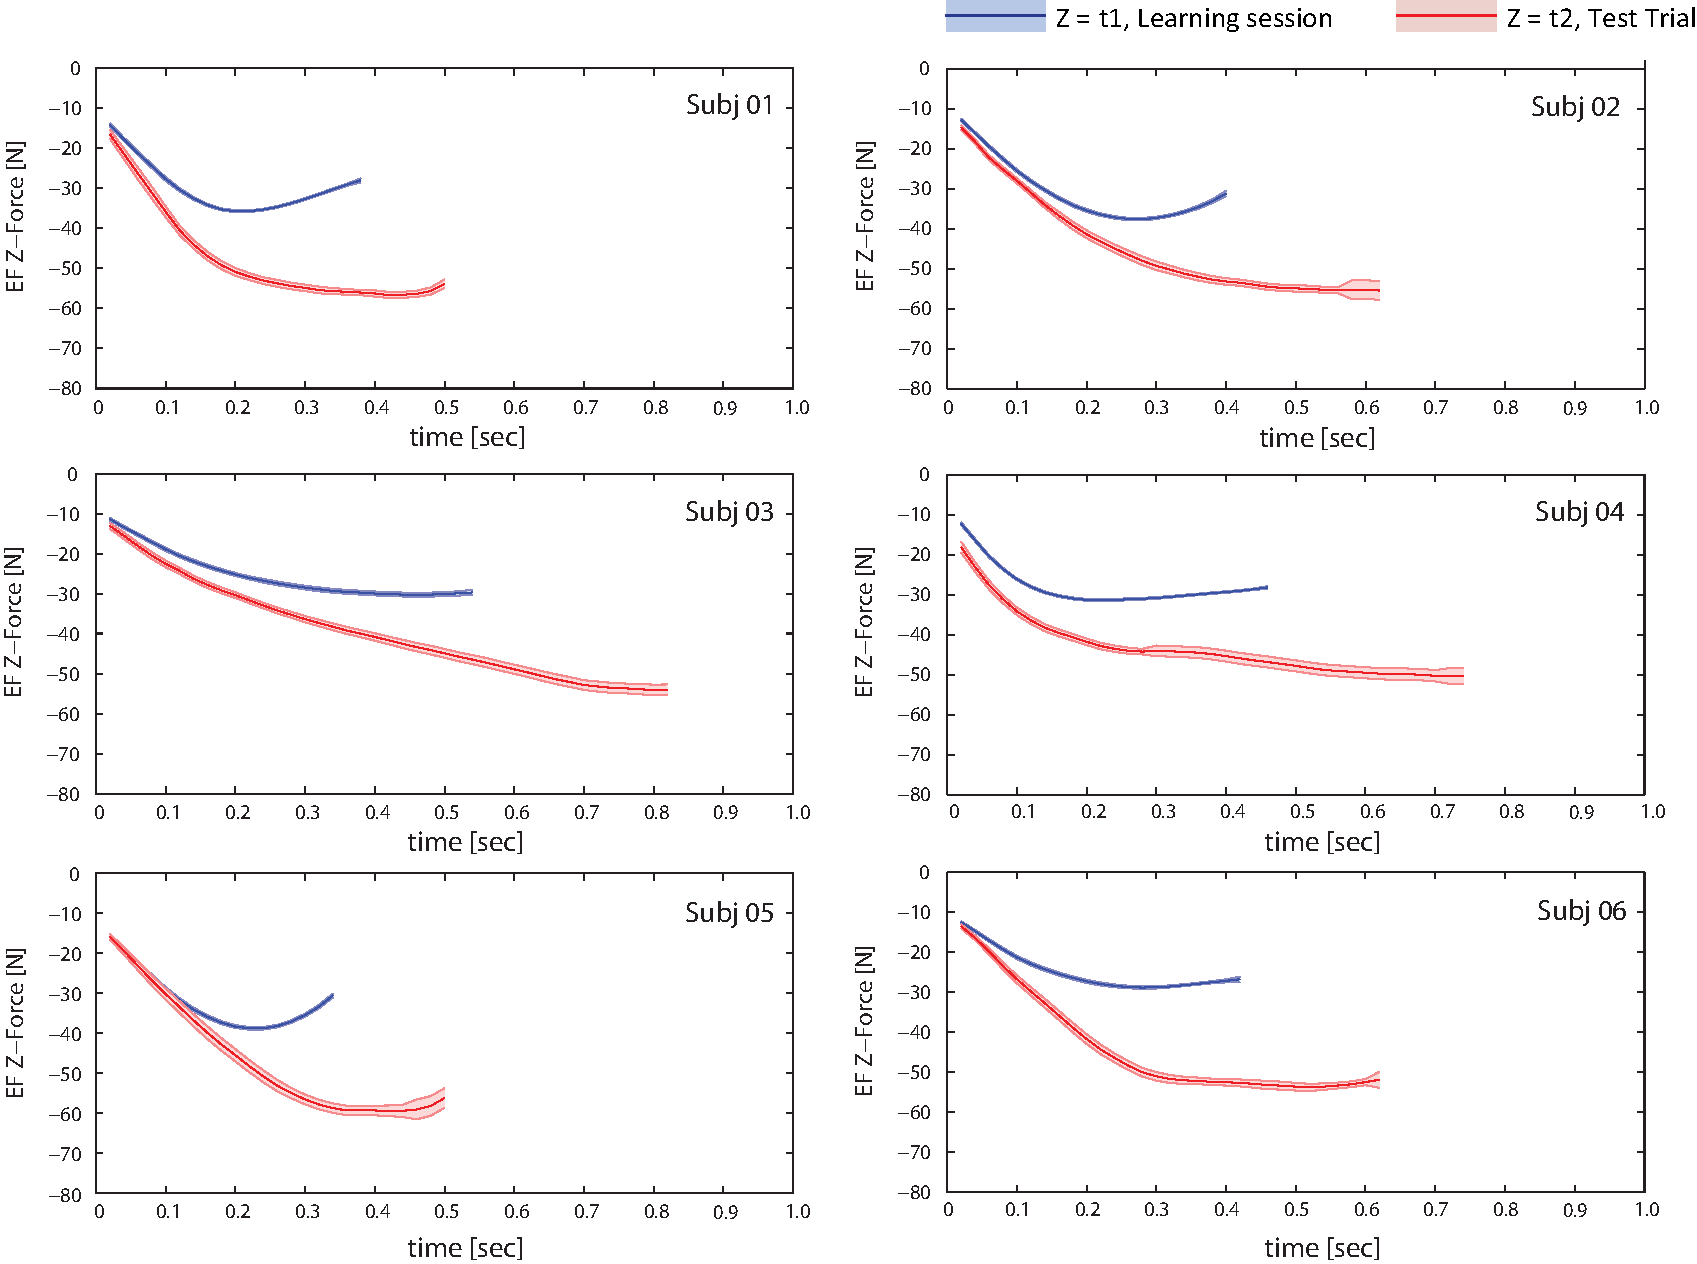
\includegraphics[scale=0.55]{fig8.pdf}
	\caption{The averaged end-effector z-force performance in the reaching movements against the linear spring-damper force for 6 subjects. The data were averaged across 3 blocks (9 (Learning + Trial) sessions). The blue lines represent the average performance in the Learning session, and the red in the Test trial, the coloured areas represent their standard error respectively.}
	\label{results_5}
\end{figure}

\begin{figure}
	\centering
	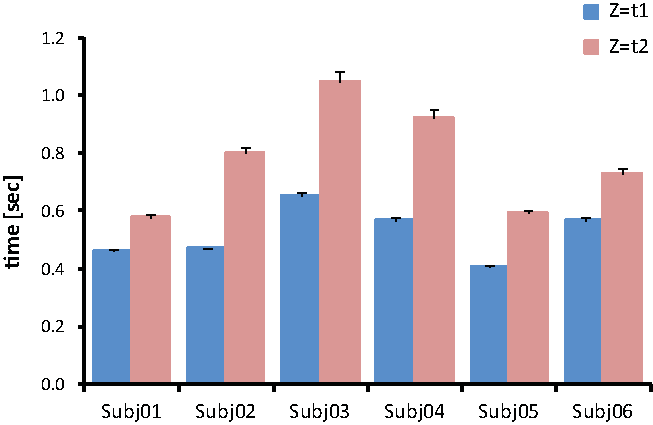
\includegraphics[scale=1]{fig9.pdf}
	\caption{Illustrate averaged time to reach the targets with the comparison between the Learning session (blue) and the Test trial (red) for six	subjects. The error bars represents the standard error across the total number of the repetitions.}
	\label{results_6}
\end{figure}


%\subsection{Brief Discussion}

\textbf{Discussion:} The \ref{results_6} showed that some participants (e.g., Subj.01, Subj.06) performed to reach the target position ($z = t_2$) much faster than the expected time duration, which was estimated from the linear equation. That is, the $t_2$ position was double distance of the t1 from the start position; so the reaching time would be estimated close to the double. The time would not be able to calculate by the simple linear calculation because the damping factor depends on the velocity, though.

This might be caused by the experimental design; that is, participants made the repetitive movements with their own rhythms at the learning session. Because they tend to keep their rhythms even in the consecutive trial session, and then they might have unconsciously increased the force or accelerated their speed to reach the target. This possibility can be seen at their movement profiles (Fig. \ref{results_4}: velocity and Fig. \ref{results_5}: force). Several studies have shown that time perception plays an important role in human motor control \cite{Berret&Jean16, Rank&DiLuca15}; therefore, this timing issue should be carefully considered into the experimental design and should avoid any confounding factors. To do this, we will visually guide the participants' movements with a certain time-windows in the future experiment.

Moreover, in the current pilot experiment, the judgment of reaching the target was inaccurate. Although the participants received the visual feedback at the learning session, it only indicated the end-effector crossed the target position, and also there were no task reward. The inaccuracy would have affected their force perception and movements \cite{Rank&DiLuca15} therefore, in the next experiment, we will set a specific correct zone visually defined by a more accurate way (e.g. the similar size of sphere of the end-effector) as the target instead of the line indicators. The task completion in the Learning session would be determined by their performance and individual learning level would be evaluated by their correct movements.

The current analyses conducted for all performance in the test trial (reaching the target ($z= t_2$) three times for each), but the performance might have needed to be evaluated focusing on the first trial only, because the first movement was directly affected by the learning session and the second and the third movements were gradually contaminated.

Overall, through the pilot experiment, we have learned the importance of the timing issue in interacting with compliant surface. We will improve the experimental design and strictly control the parameters (timing, speed, and the accuracy). 

In the future experiment, based on the linear case, we will measure the pattern under the non-linear compliant forces and examine the human goal-directed performance. Besides, as well as the spring-damper, it may help the understanding of the generalization if we employ another compliant force model (e.g. object surface).



\subparagraph{Experimental validation of CoM manipulability metric (Task 2.2 \& Task 2.3)}

After the introduction of a set of metrics for studying, analyzing and measuring the ability of humans and humanoids to balance, we performed an experimental study to verify the application of this metrics for human postural control in contact with the environment. In the experiments, the posture of human subjects were perturbed in different configurations and joint torques were computed by inverse dynamics calculations. We demonstrated that the metric is suitable for comparing different postures in the sense of the total required effort for the maintenance of balance.


\textbf{Human experiments:} To verify the application of the \textit{change-of-velocity---unit joint 	impulse} ellipsoid for human studies, we performed experiments on human subjects. As already mentioned, this ellipsoid can be used to measure torque efficiency in balancing motions. So, in the experiments, we perturbed the CoM of the subjects (by a cable-pulley mechanism) in different configurations and measured the contact forces/moments with force/torque sensors (see Fig.~\ref{experimentsetup}). Then we calculated the average total torque that was done by the subjects at each configuration and compared them with the results of manipulability analysis. These steps are described in the following subsections.

\begin{figure}
	\centering
	\begin{tabular}{c}
		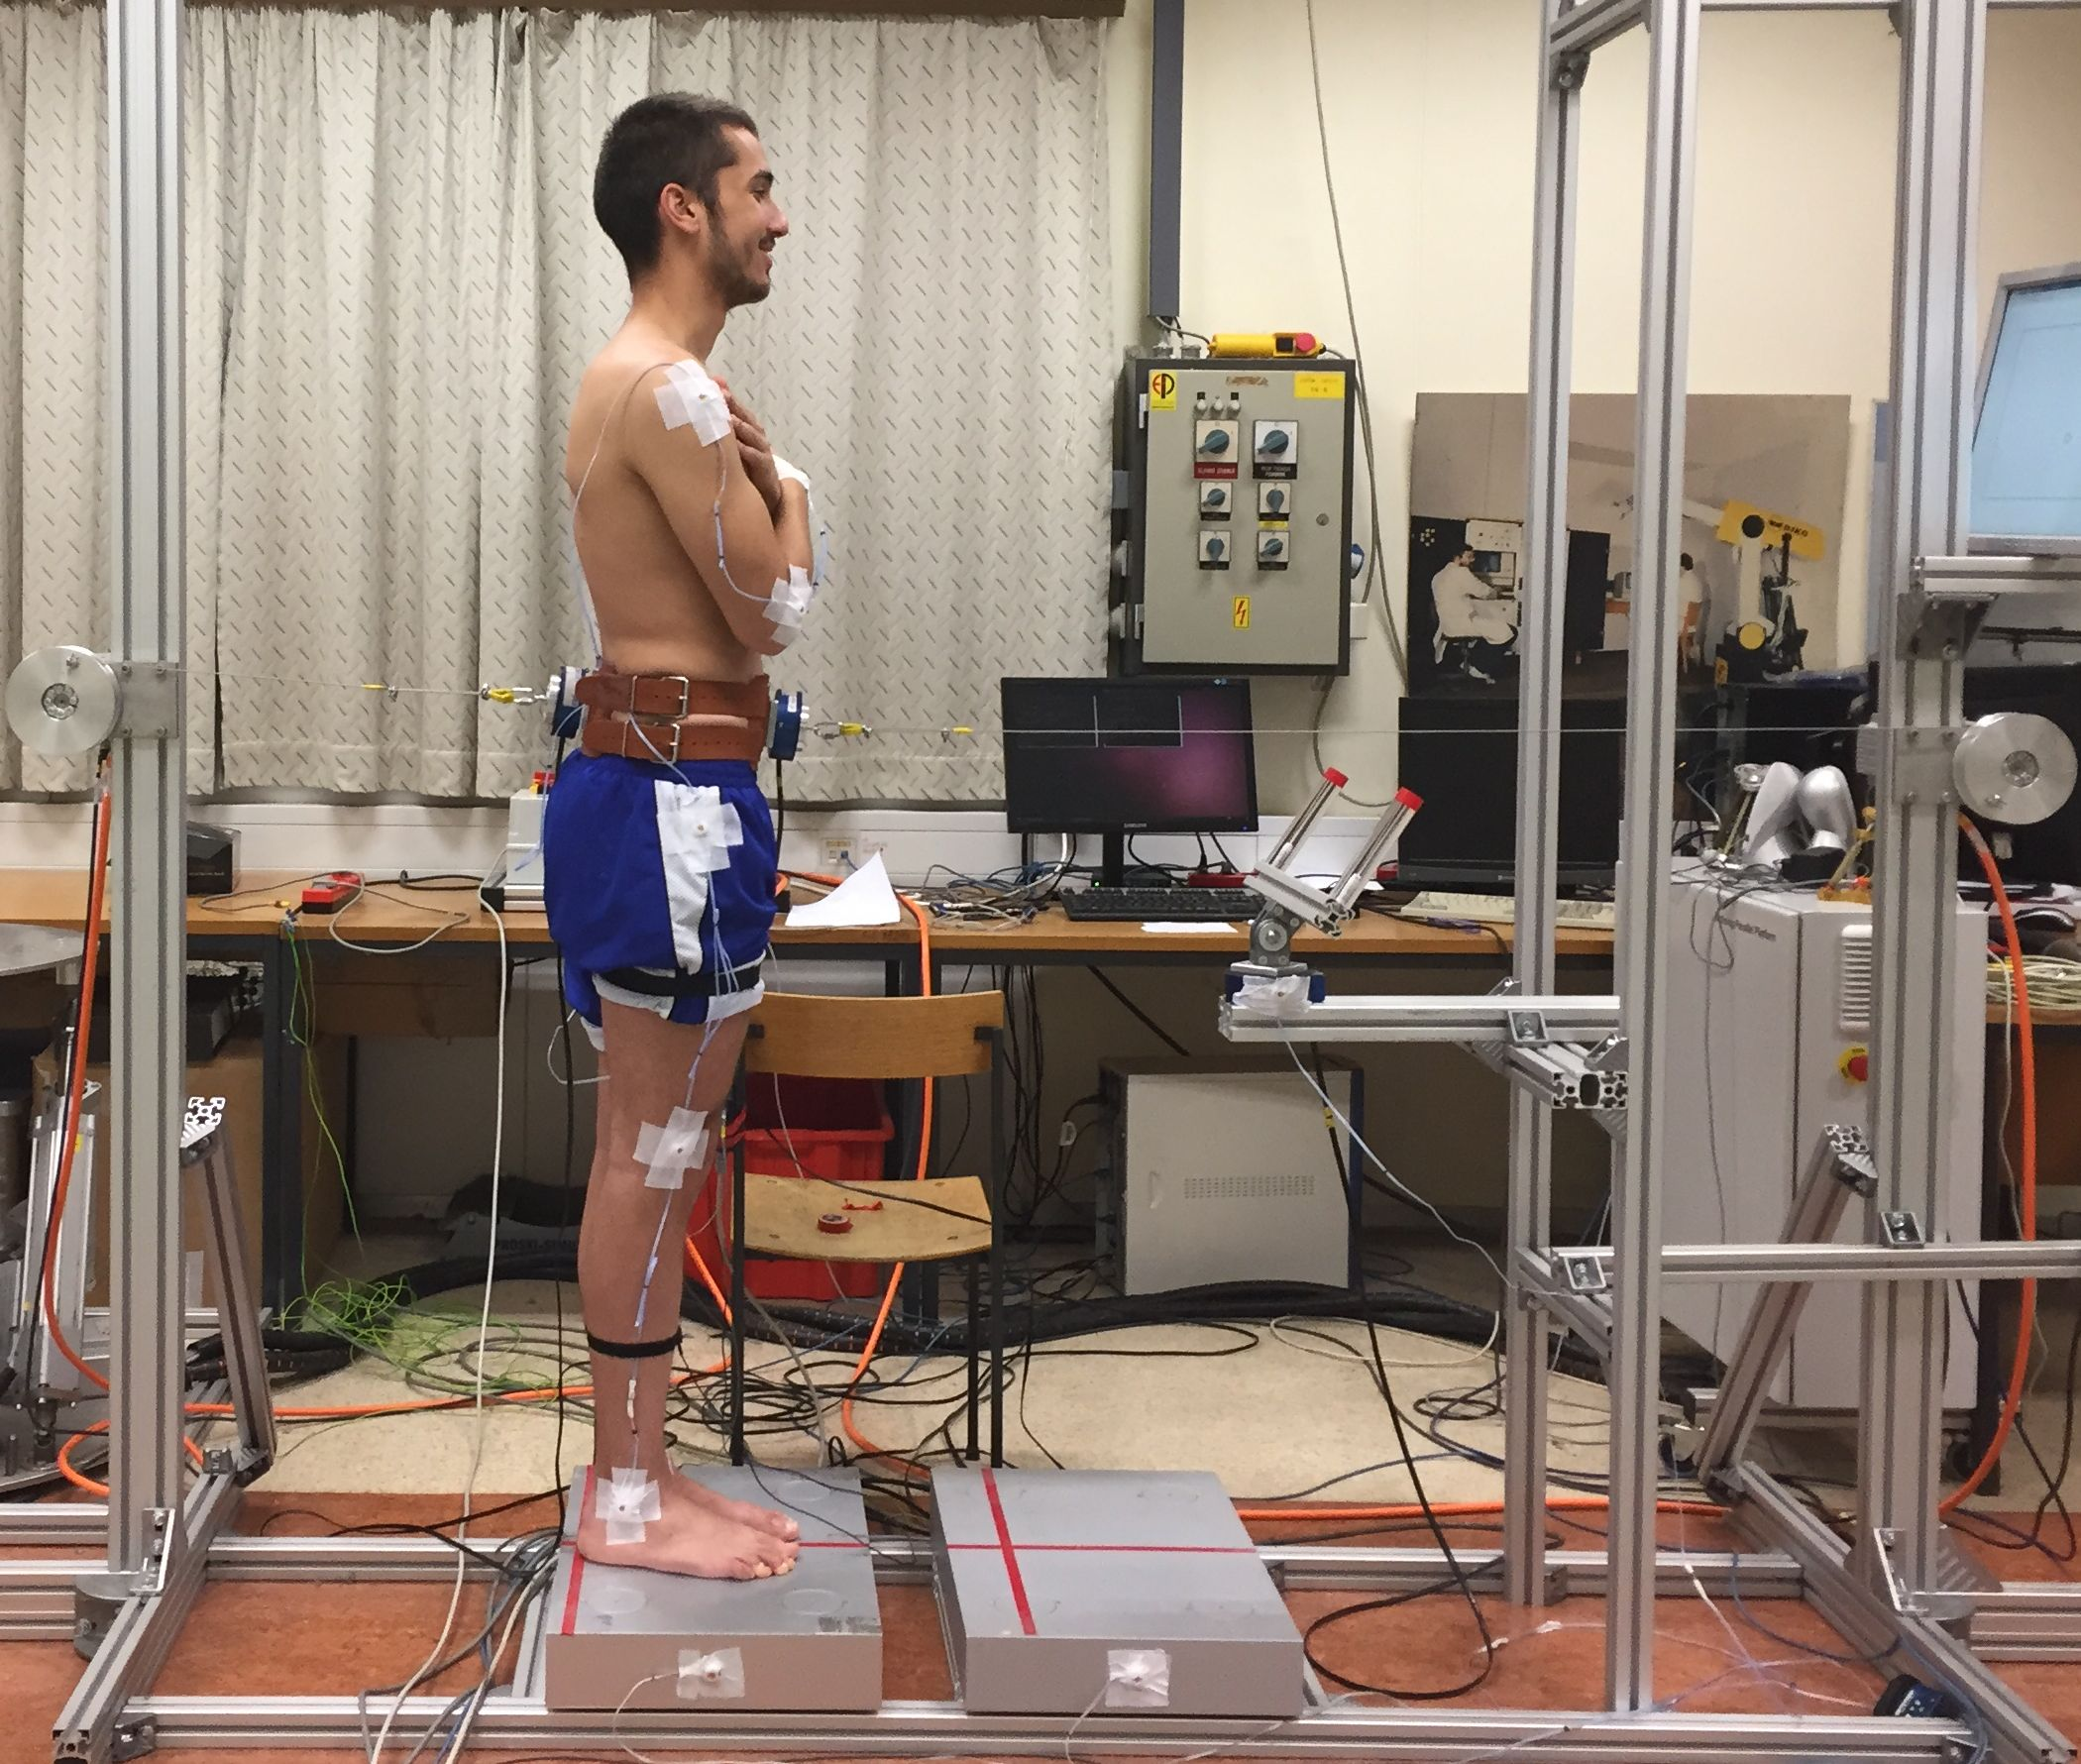
\includegraphics[width=0.75\columnwidth]{stance.jpg} \\
		(a)\\
		
	\end{tabular}
	\centering
	\begin{tabular}{cccc}
		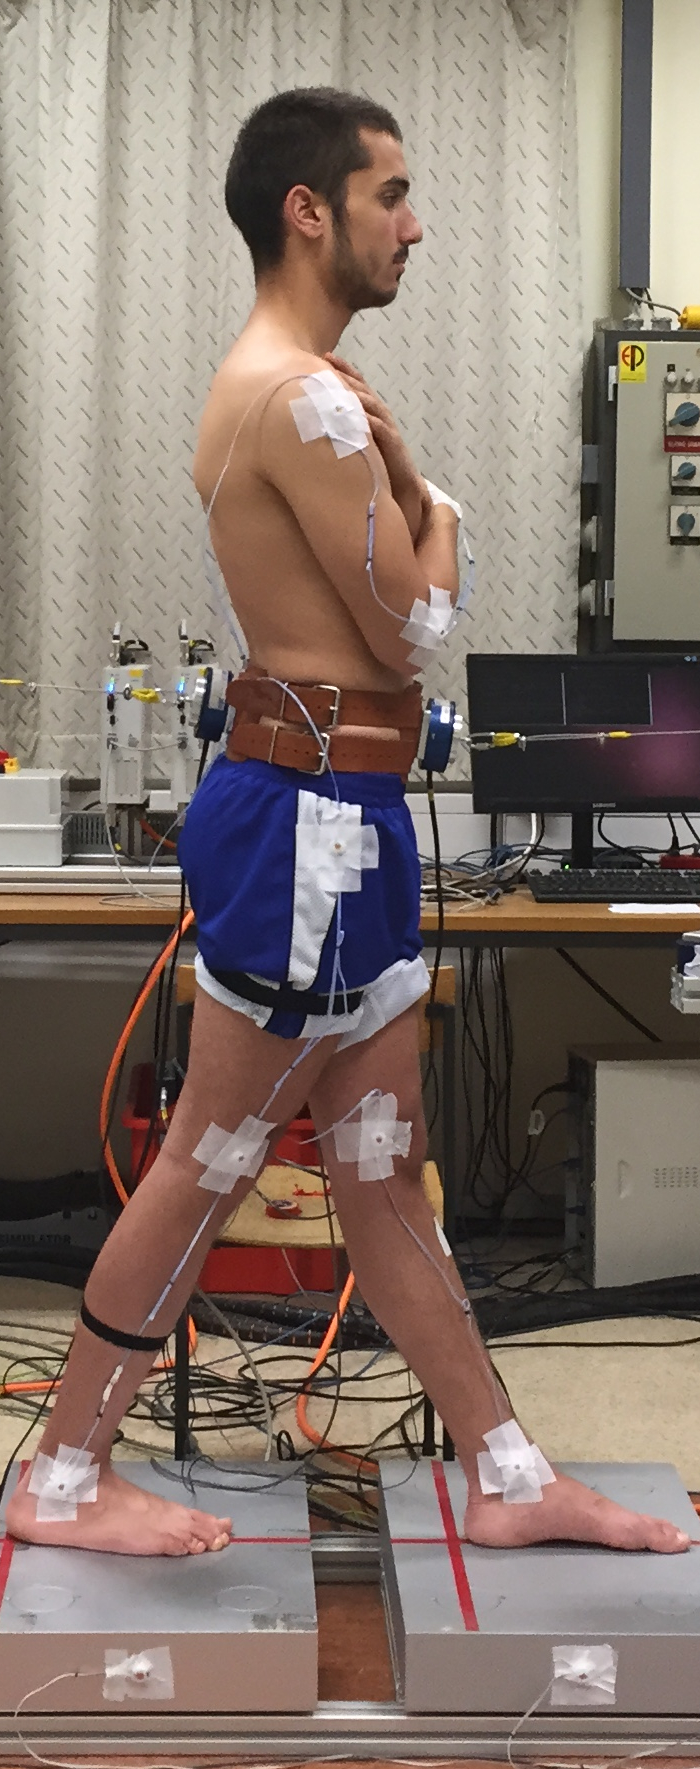
\includegraphics[width=0.2\columnwidth]{widestance.jpg} &
		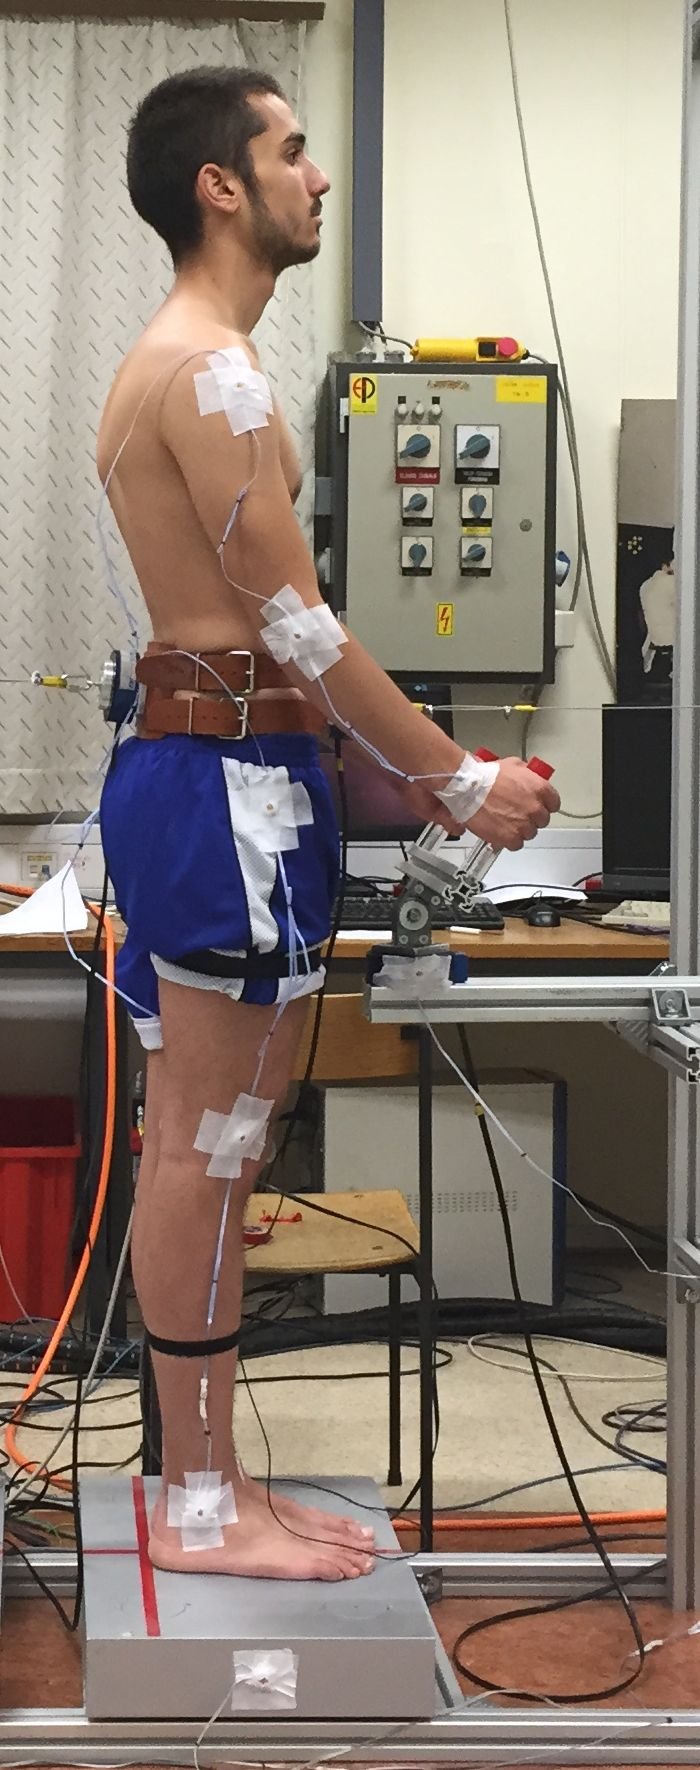
\includegraphics[width=0.2\columnwidth]{low.jpg} &
		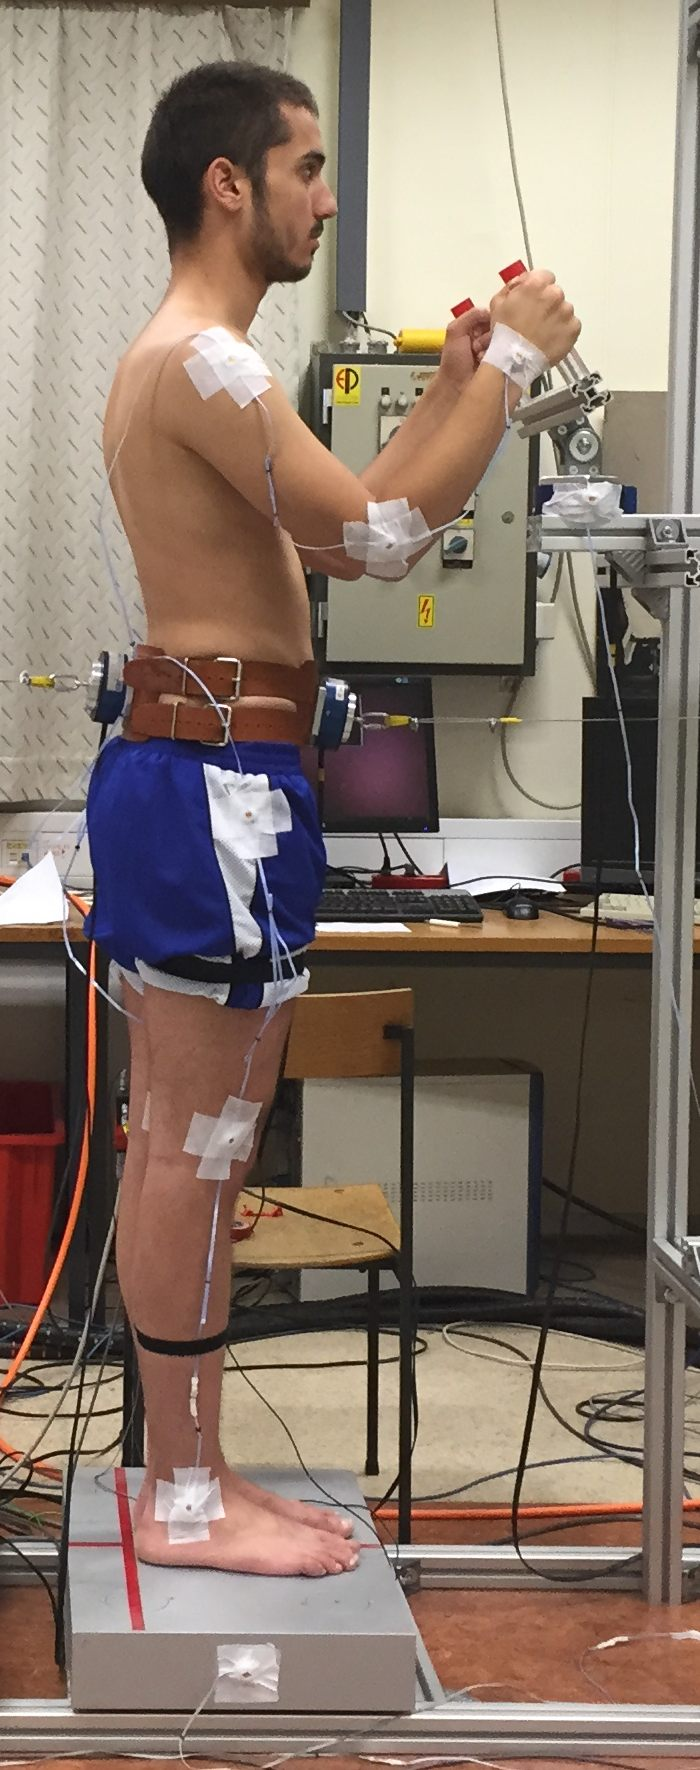
\includegraphics[width=0.2\columnwidth]{mid.jpg} &
		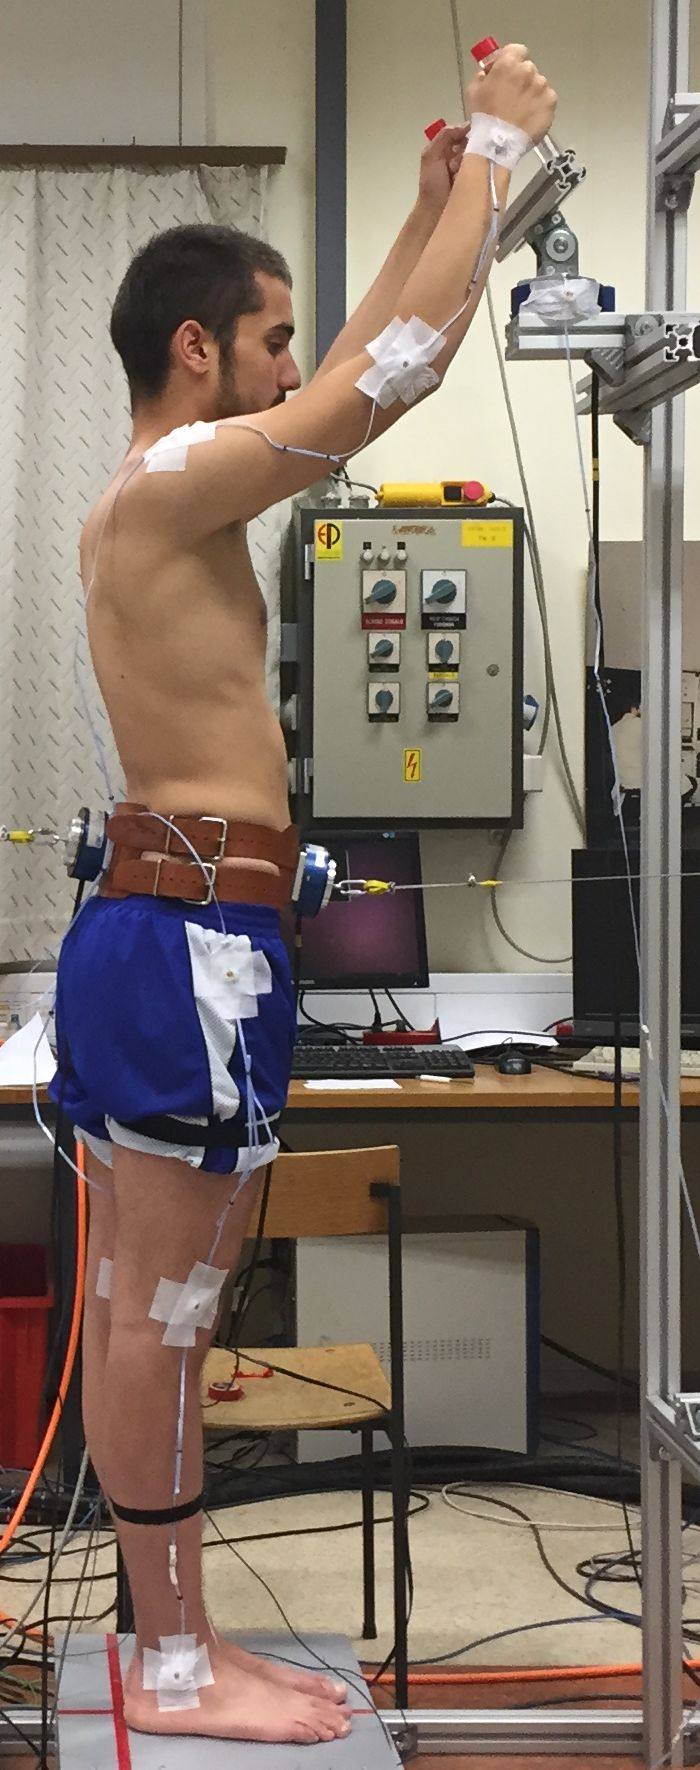
\includegraphics[width=0.2\columnwidth]{high.jpg} \\
		(b) & (c) & (d) & (e)
	\end{tabular}
	\caption{Experiments setup for five different positions: (a) stance, (b) wide stance, (c) low handle, (d) middle handle and (d) high handle. A pulley mechanism, which is connected to the subject by a belt, perturbs the subject's CoM. Contact forces are measured at the feet and hands. Motion is recorded with an optical motion capture system.}
	\label{experimentsetup}
\end{figure}


\textbf{Methods:} Eleven healthy male subjects participated in this study. Their average age was $21.7$ years (SD $=2.2$ years), height = $183$ cm (SD $=4.6$ cm) and body mass $76.8$ kg (SD $=8.1$ kg). The subjects were informed about the course of the study prior to their participation and were required to sign an informed consent approved by the National Medical Ethics Committee (No. 112/06/13).

We observed the subject’s reactions to the external perturbations in five different poses. In the first pose (\textit{stance}), subjects were standing straight with their feet together and arms crossed over the torso (Fig.~\ref{experimentsetup}.a). In the second pose (\textit{wide stance}), subjects were standing with their arms crossed over the torso and their left foot $60$ cm ahead of their right foot (ankle to ankle distance). In the third pose (\textit{low handle}), subjects were standing as in the first pose and holding the handle which was located in front of their bodies at the hip height (Fig.~\ref{experimentsetup}.b). In the fourth pose (\textit{middle handle}), subjects were standing as in the first pose and holding the handle which was located in front of their bodies at the shoulder height (Fig.~\ref{experimentsetup}.c). In the last pose (\textit{high handle}), subjects were standing as in the first pose and holding the handle which was located in front of their bodies and above the head (Fig.~\ref{experimentsetup}.d).

The subjects were perturbed by a horizontal external force produced by our force-controlled pulling mechanism \cite{Peternel&Babic13} at the approximate position of their CoM \cite{Gardetal04}. The command signal was a step with $0.5$ second width (see Fig.~\ref{perturbations}). The actual perturbation force was controlled by a combination of a feed-forward and a PID feedback controller. We selected eight linearly increasing magnitudes of perturbation forces where the maximum was defined as 22\% of the individual subject's body weight and the minimum was $1/8$ of the maximum force (increasing rate of $1/8$ of the maximum). Between each perturbation we induced a random pause. For each pose, we repeated the series of eight perturbations ten times (80 trials per subject per pose) and observed the human reactions. We gave the subjects 10 minutes pause between each pose. In case of the first pose, the subjects had to step before the maximum perturbation was reached. When the
subject made a step, the experimenter stopped the procedure and moved to the next series of perturbations. The step was not required in other poses and the series of perturbations repeated uninterrupted.
\begin{figure}
	\centering
	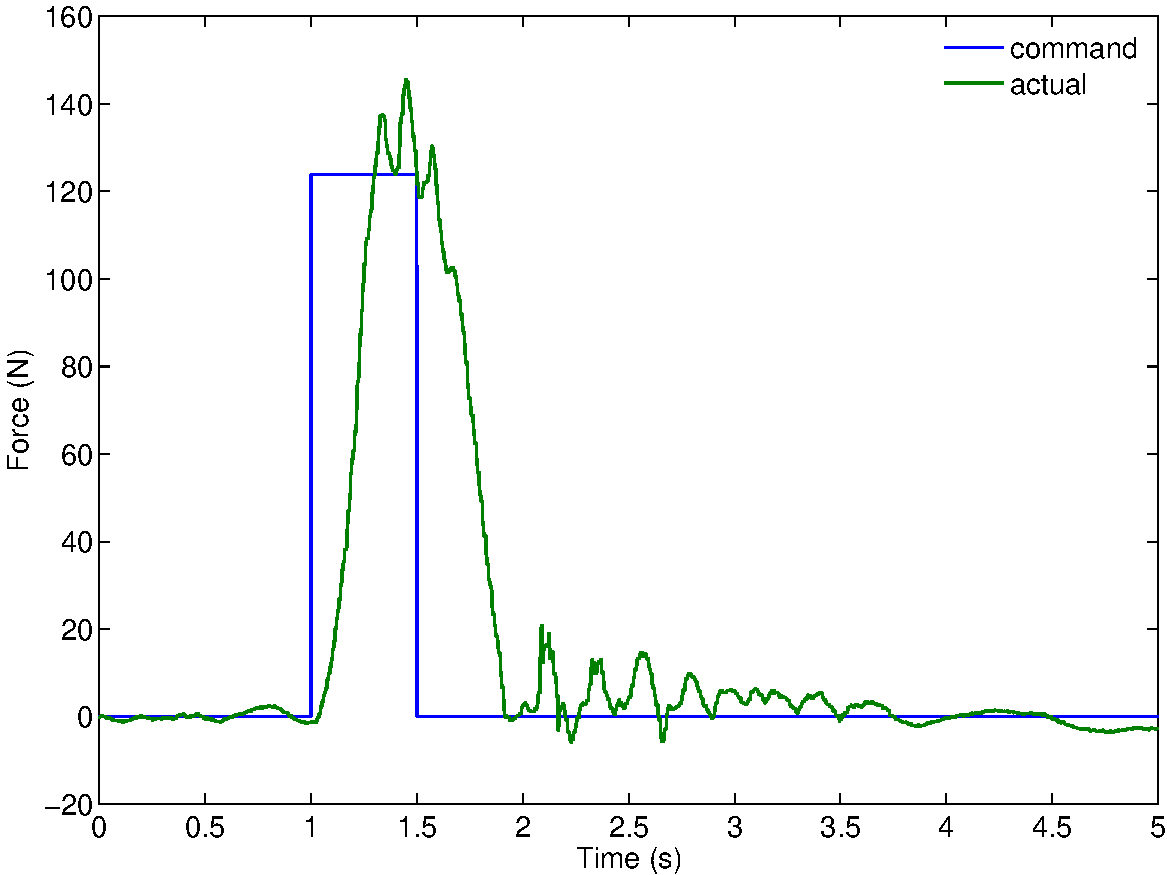
\includegraphics[scale=0.4]{perturbation.pdf}
	\caption{An example of the perturbation force applied to the CoM of the subjects. This is for the subject whose body mass is $76.5$ kg. The intensity of the perturbation is number $6$ meaning that the force is 	$6/8$ of the maximum for this subject.}
	\label{perturbations}
\end{figure}

Body movements were measured by a motion capture system (3D Investigator$^{\tt\small TM}$ Motion Capture System, NDI, Waterloo, Ontario).The optical markers were placed on the ankle, knee, hip, shoulder, elbow and wrist. The positions of the markers are used to calculate the joint angles. We used two force plates (9281CA, Kistler Instrument AG, Winterthur, Switzerland) to measure the ground reaction forces and center of pressure position. The handle was mounted on a 3-axis force sensor (45E15A, JR3, Woodland, USA) to measure the force between the handle and the subject.

In order to estimate the starting time of the subjects' reactions, we measured muscle activation in Triceps Brachii, Soleus and Tibialis Anterior by surface electromyography (EMG). We placed surface EMG electrodes (SX230 EMG sensor,Biometrics Ltd, Newport, UK) on the selected muscles in accordance with SENIAM recommendations \cite{Hermensetal99}. We also placed a monitor in front of the subject to provide visual feedback on the CoP position that allowed him to move back to the initial pose after each perturbation.


\textbf{Model:} In the experiments, in order to produce movements which are planar only, we prevented applying out-of-plane forces/moments to the subjects by providing a pair of handles for them and perturbing them in a plane. Therefore, we could use planar models for both inverse dynamics and CoM manipulability calculations. Although, using a planar model for wide stance pose is a bit unrealistic. Planar humanoid models that we used for the stance, wide stance and all three handle poses are shown in Fig.~\ref{planarhumanoids}. These models consist of multiple links which are connected to each other by actuated revolute joints. Note that lower legs are connected to the ground. This is because we assume that the feet of the subjects do not move during the experiments. To model the stance pose, we lock the DoF of the arms. So, in this case, the model has 3 DoF and is unconstrained. For the wide stance, the robot has 6 DoF and is constrained due to the kinematic loop in the legs. For the handle poses, the robot has five actuated DoF and it is constrained at the hand to model the handle contact.
\begin{figure}
	\centering 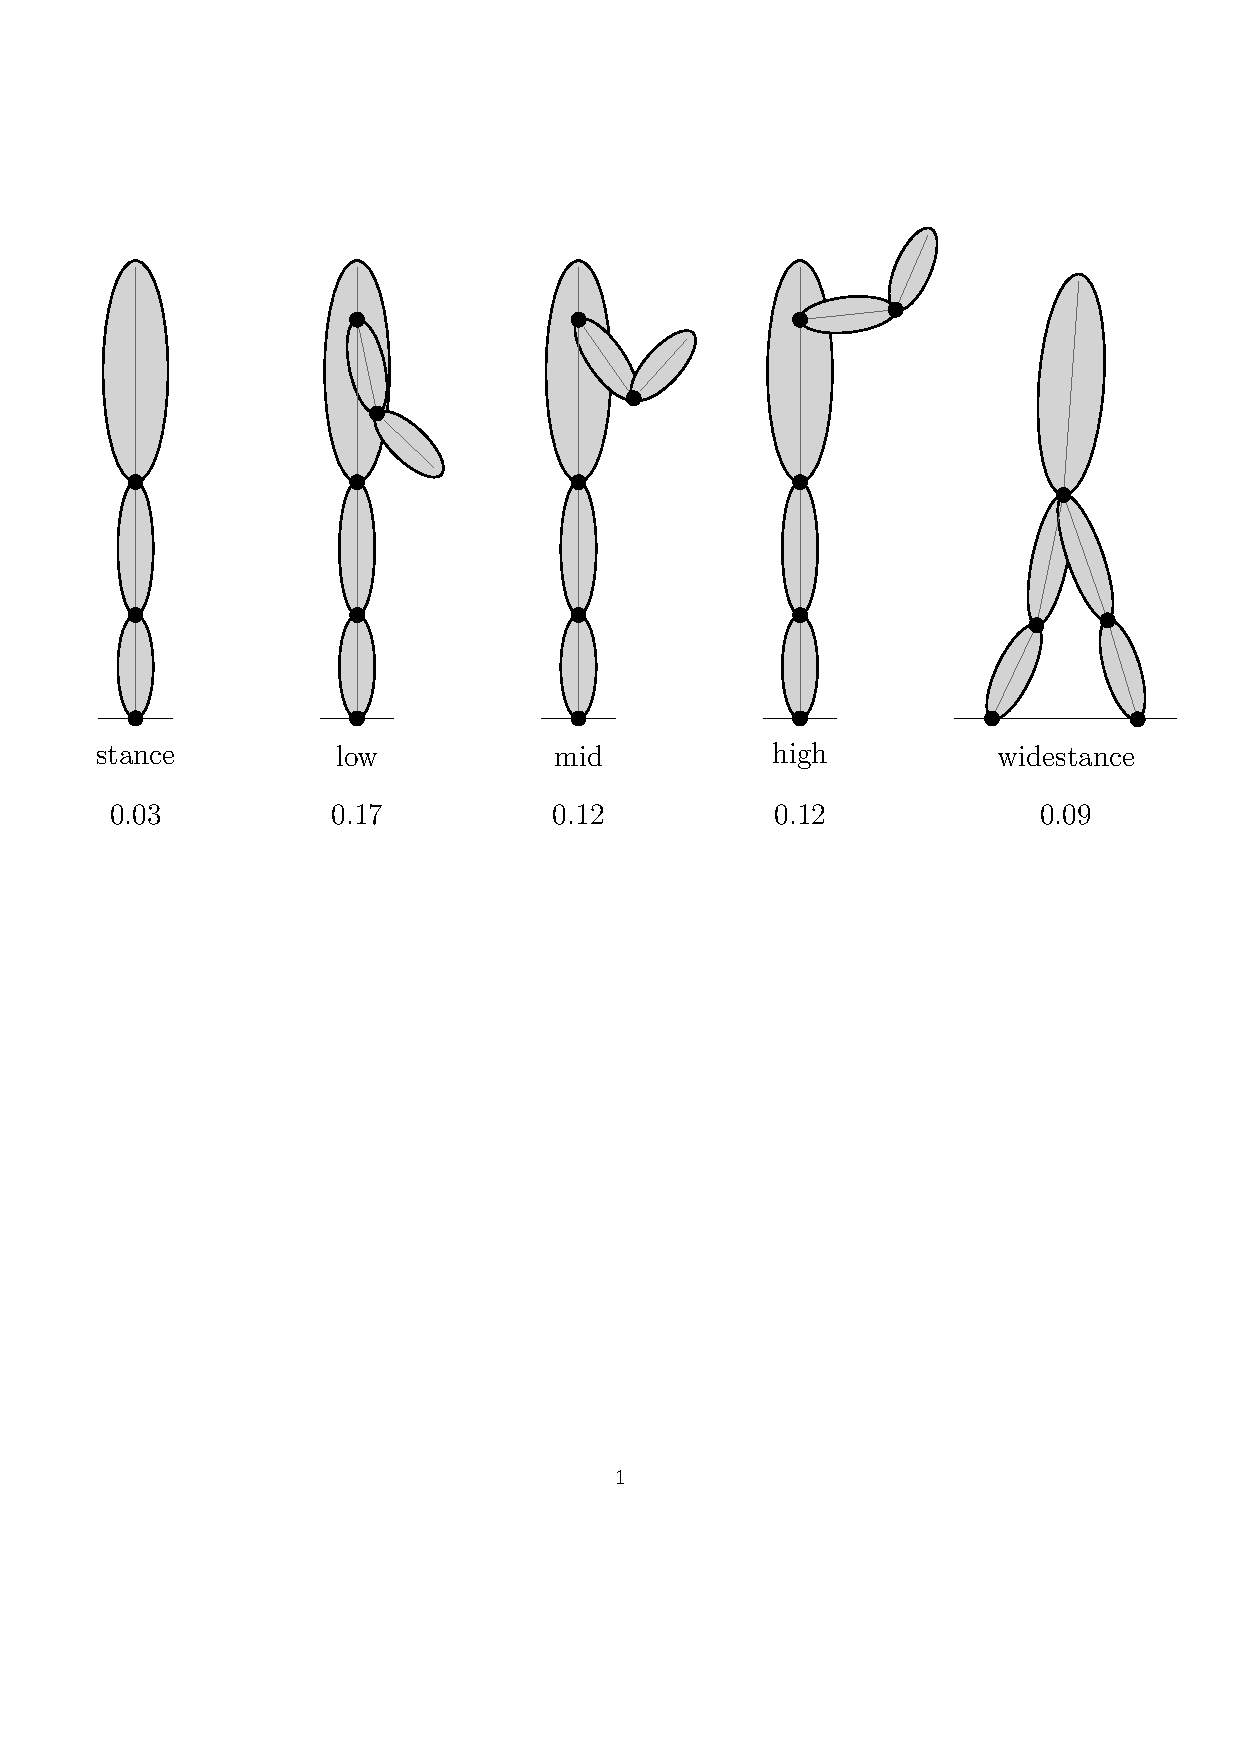
\includegraphics[trim = 13mm 154mm 10mm 37mm, clip,
	scale=0.85]{robotmodels}
	\caption{Schematic diagram of the planar humanoid robot model.}
	\label{planarhumanoids}
\end{figure}

Since for balancing we are only interested in movements in the horizontal direction, we calculated the maximum value of $\Delta \dot{\Bc}$ in this direction for all five positions. This represents the maximum achievable change of velocity of the CoM in the horizontal direction and is a measure for the ability to accelerate the CoM in order to correct its position in this direction. Joint angles of the arms for the handle positions are set to the average initial joint angles of the subjects that we calculate from the marker positions. For the low handle, the shoulder angle (angle between torso and upper arm) is $12^\circ$ and the elbow angle (between upper and lower arms) is $145^\circ$. Shoulder and elbow angles are $35^\circ$ and $77^\circ$ for the middle handle, and $96^\circ$ and $118^\circ$ for the high handle positions, respectively. For the wide stance position, we assume zero angles in the knees and upright torso. The weighting matrix that we use for the calculations is a diagonal matrix as
%
\begin{equation}
\BW = diag([2.33, 3.45, 4.55, 1, 1.25]) \, ,
\end{equation}
%
which is determined to include the differences in the joint's strengths \cite{Anderson2007, Bober2002, Gandevia1998, Moraux2013}.

Calculated values for the maximum $\Delta \dot{\Bc}$ for the five positions are mentioned in Fig.~\ref{planarhumanoids}. As it can be seen in this figure, the low position has the highest value (i.e. $0.17$) for the manipulability and the stance position has the lowest one (i.e. $0.03$). Manipulability for the middle and high positions are the same ($0.12$) and lower than the low position. Also wide stance manipulability (i.e. $0.09$) is only better than the stance position. Therefore, according to the manipulability analysis for our models, we expect the same ranking for the five positions in the sense of total average required torque to keep the balance. We will verify this hypothesis in the next subsection.


\textbf{Results:} As already mentioned, inverse dynamics are used to compute the torques that are applied (at the joints) by the human subjects. Joint angles are calculated by using marker positions, and joint velocities and accelerations are estimated by using simple time differentiation. Lengths and inertial parameters of the subjects are calculated via the software that is introduced in \cite{Zlajpah&Babic14}. Feather stone's Spatial software package \cite{Featherstone} is used for the dynamics calculations.

To work out the average total torque for each position and each perturbation intensity, first we calculate the joint torques from inverse dynamics for each trial (in total $4400$ trials $= 5$ poses $\times 8$ intensities $\times 10$ reps $\times 11$ subjects). Then we calculate the average torque over the reps for each joint. Note that, since maximum achievable torque of the arm joints vary with arm configuration, we normalize shoulder and elbow torques for the handle positions \cite{Anderson2007, Bober2002, Gandevia1998, Moraux2013}. Then, we sum up the normalized joint torques to get $440$ (i.e. $5$ poses $\times 8$ intensities $\times 11$ subjects) values for the average normalized joint torques. The beginning time is the subjects' average initial reaction time which is estimated by the average EMG signal. The end time is roughly the time that the subjects have recovered from the perturbations.

%The same process gives us the average joint works.  The work is in fact the
%sum of $|\Btau \dot{\Bq}| \Delta t$, where $\Delta t$ is the data gathering
%frequency which is 2 milliseconds in our experiments.  We take the sum from
%$t=1.2$ s to $t=3$ s.

%% The values of the calculated normalized joint torques for the five positions
%% and different perturbation intensities are shown in
%% Fig.~\ref{jointtorquesubjects} for all subjects.  These values are marked by
%% $+$ In The graphs.  The Lines in the graphs are fitted to the values by using
%% least squares method.  Note that the graph of the first subject does not
%% include the results for high handle position.  This is due to the problem in
%% data gathering during the experiment which is solved for the next subjects.
%% \begin{figure}
%%   \centering
%%   \begin{tabular}{cc}
%%     subject 1 & subject 2 \\
%%     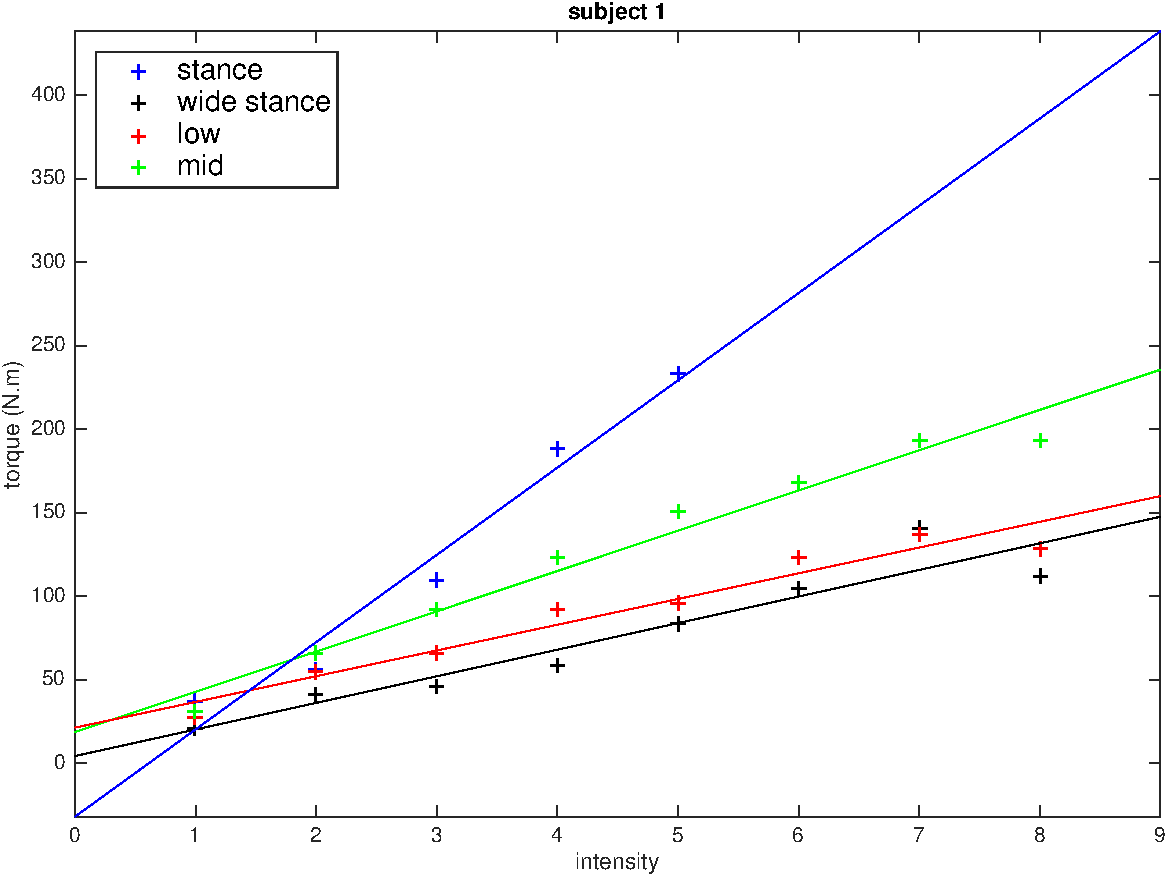
\includegraphics[width=0.46\linewidth]{subj1} &
%%     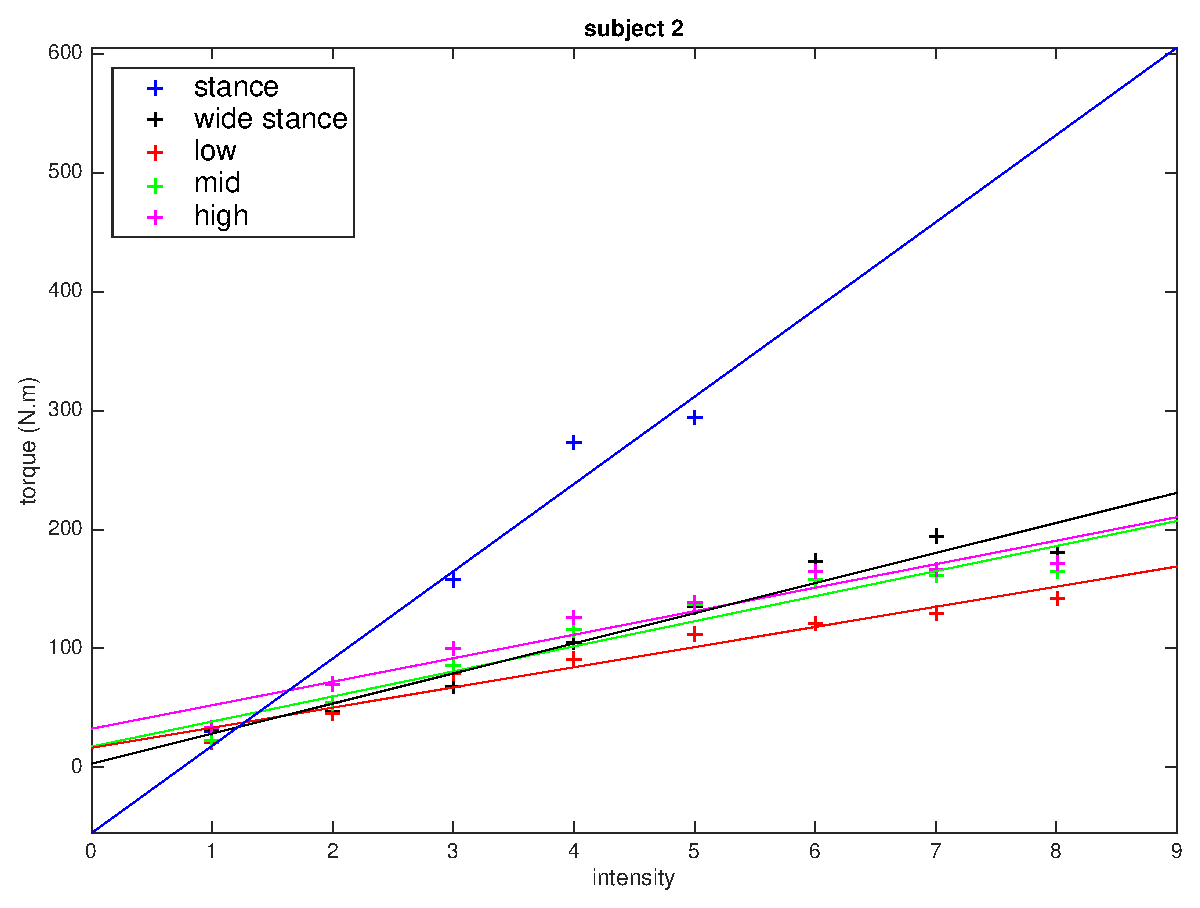
\includegraphics[width=0.46\linewidth]{subj2} \\
%%     subject 3 & subject 4 \\
%%     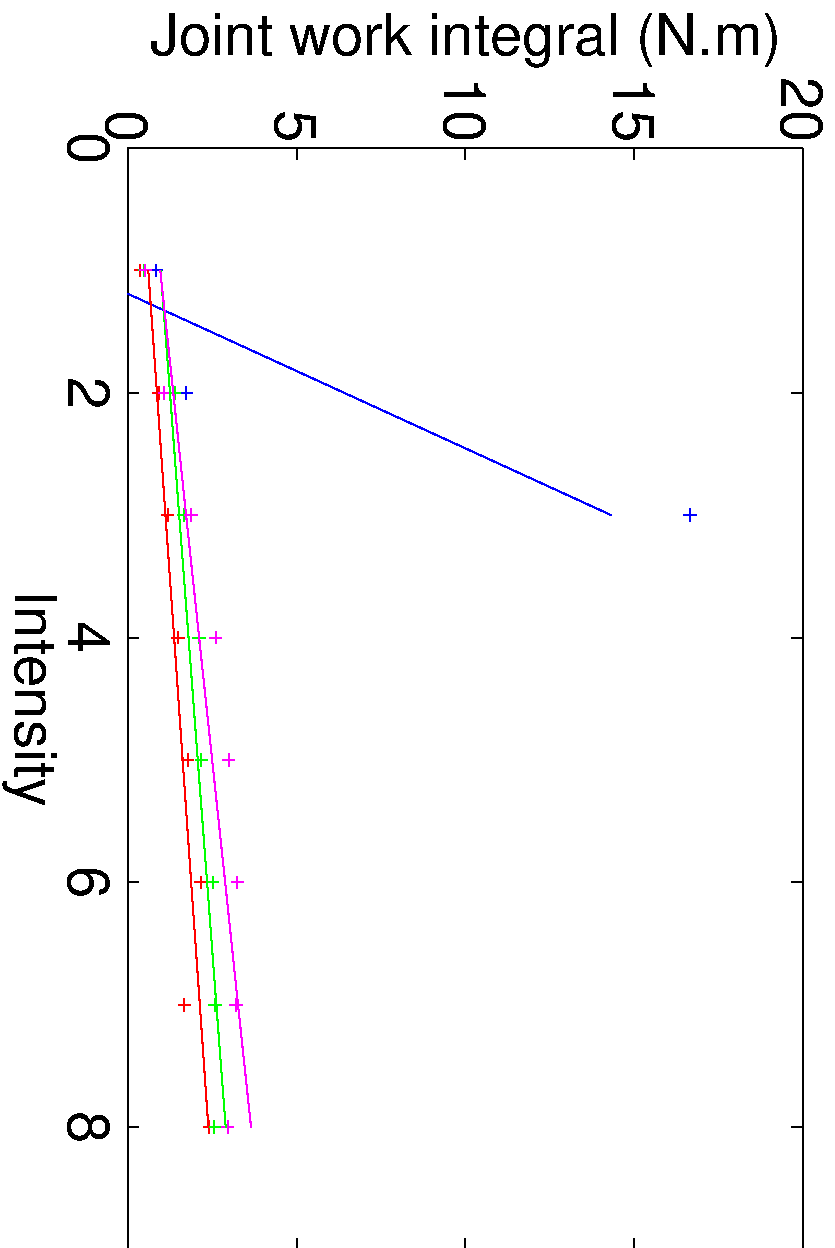
\includegraphics[width=0.46\linewidth]{subj3} &
%%     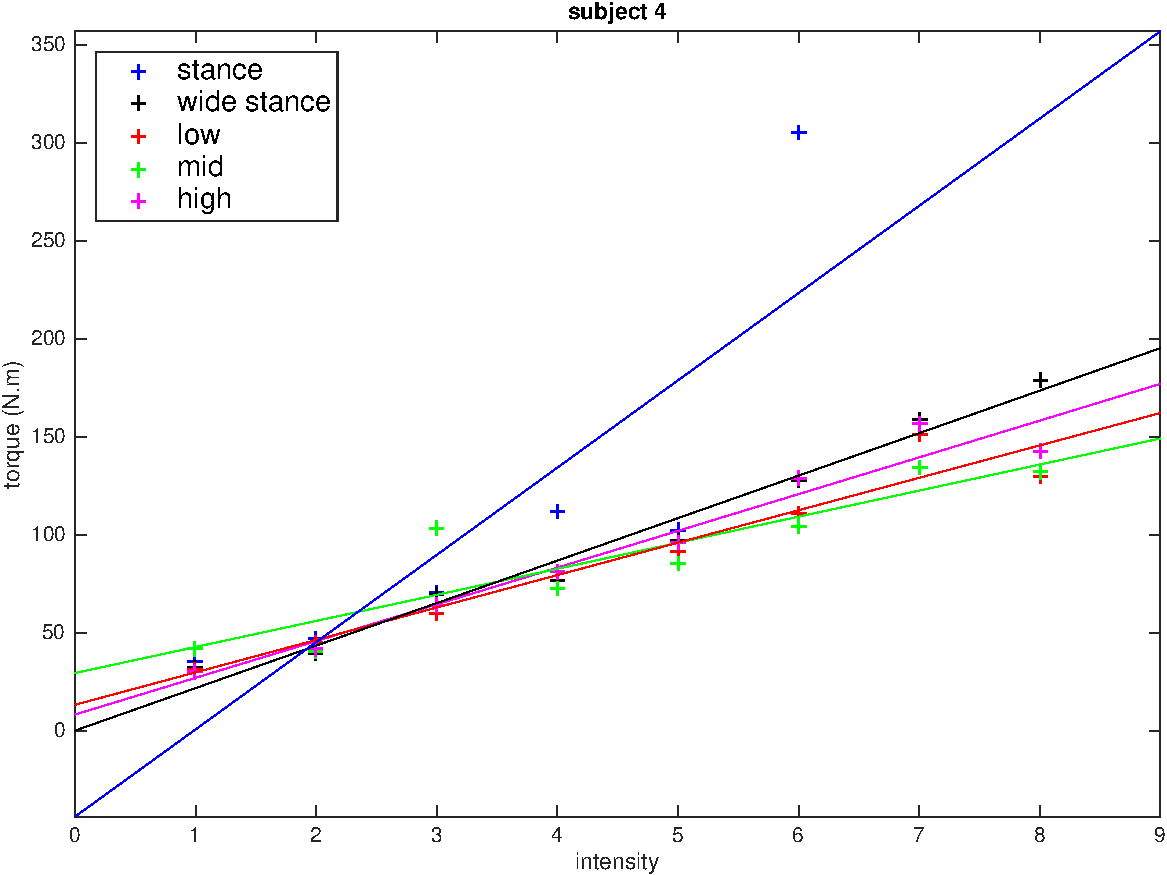
\includegraphics[width=0.46\linewidth]{subj4} \\
%%     subject 5 & subject 6 \\
%%     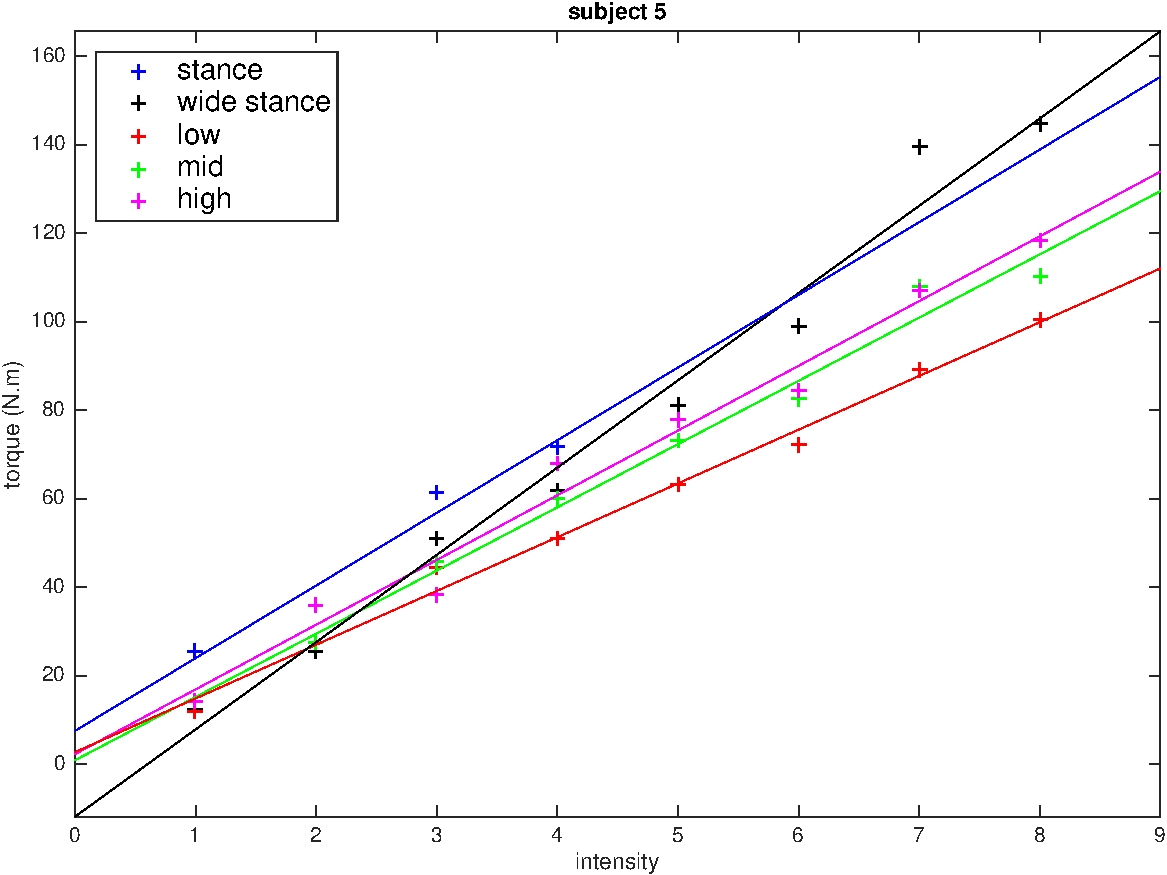
\includegraphics[width=0.46\linewidth]{subj5} &
%%     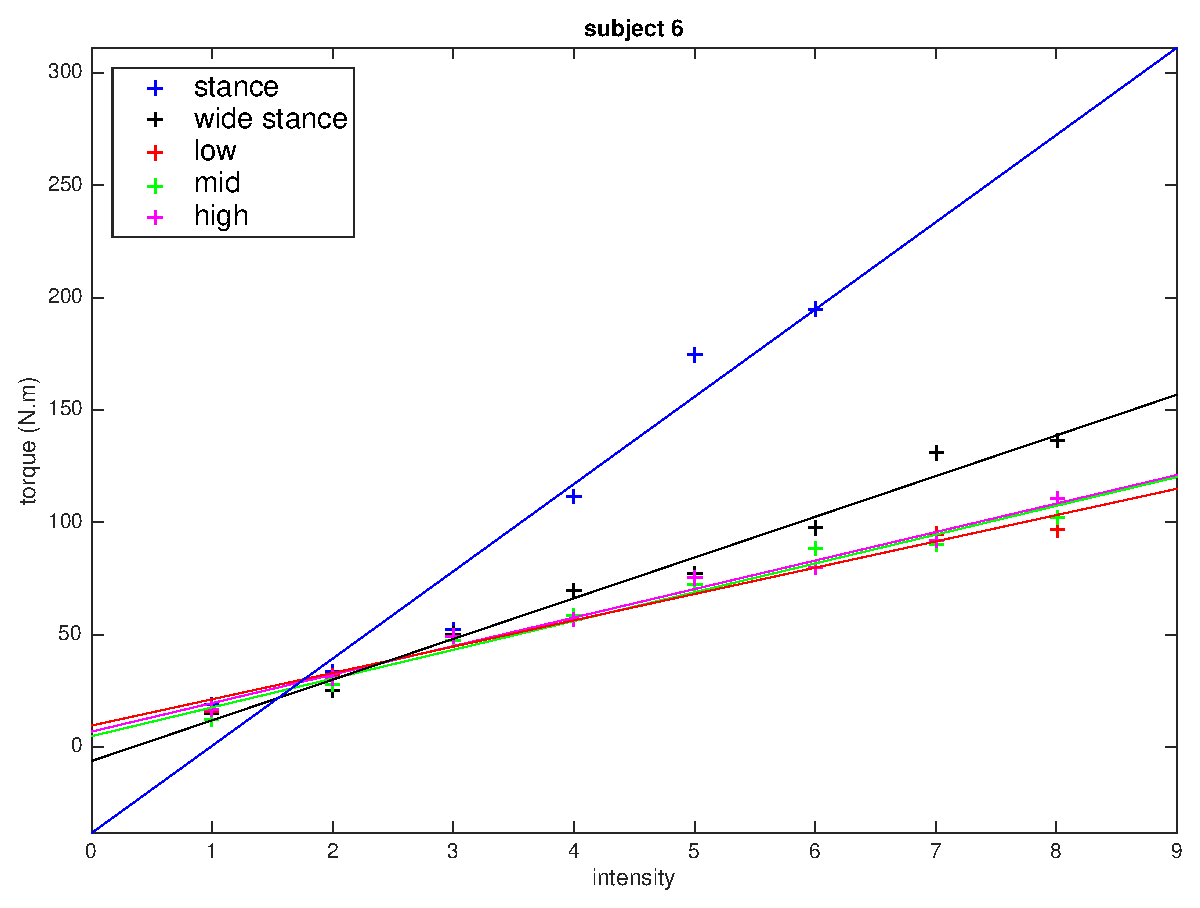
\includegraphics[width=0.46\linewidth]{subj6} \\
%%     subject 7 & subject 8 \\
%%     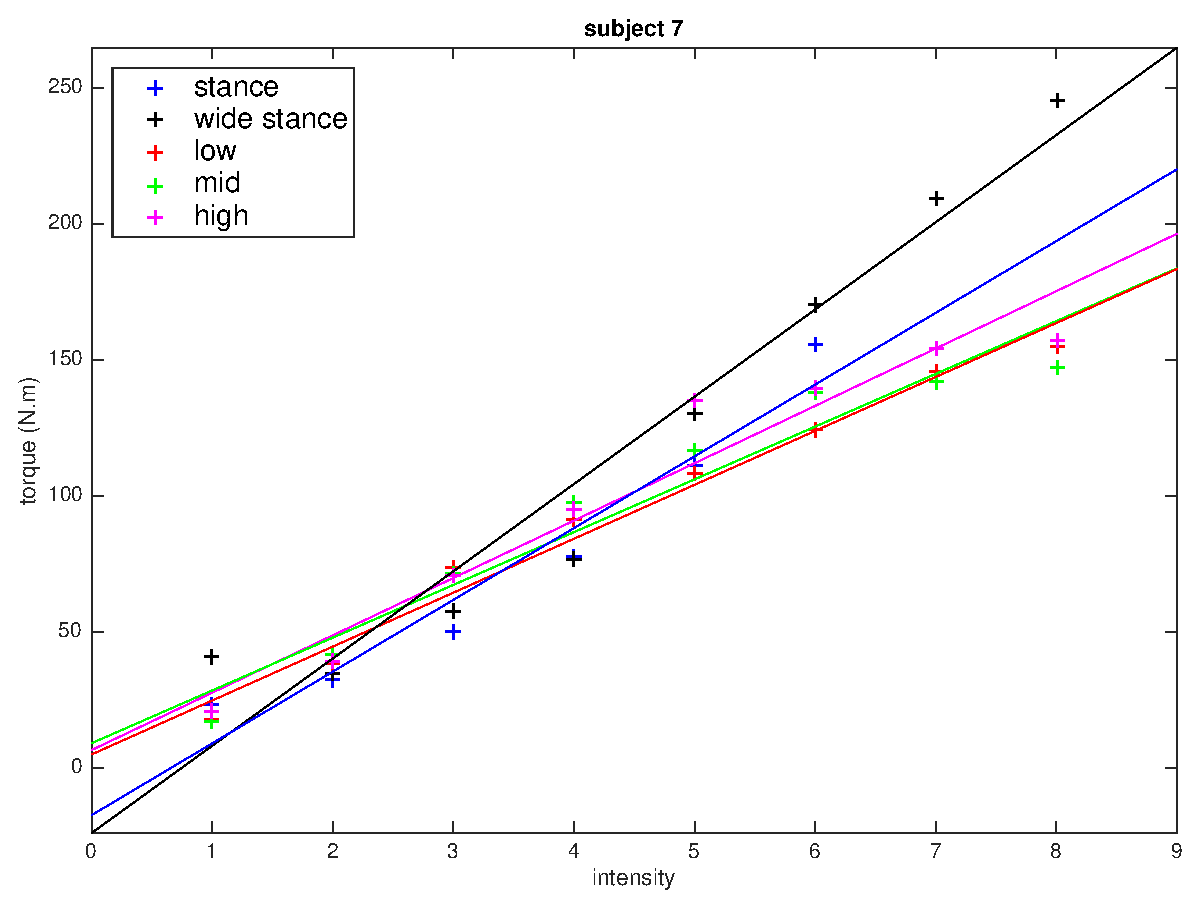
\includegraphics[width=0.46\linewidth]{subj7} &
%%     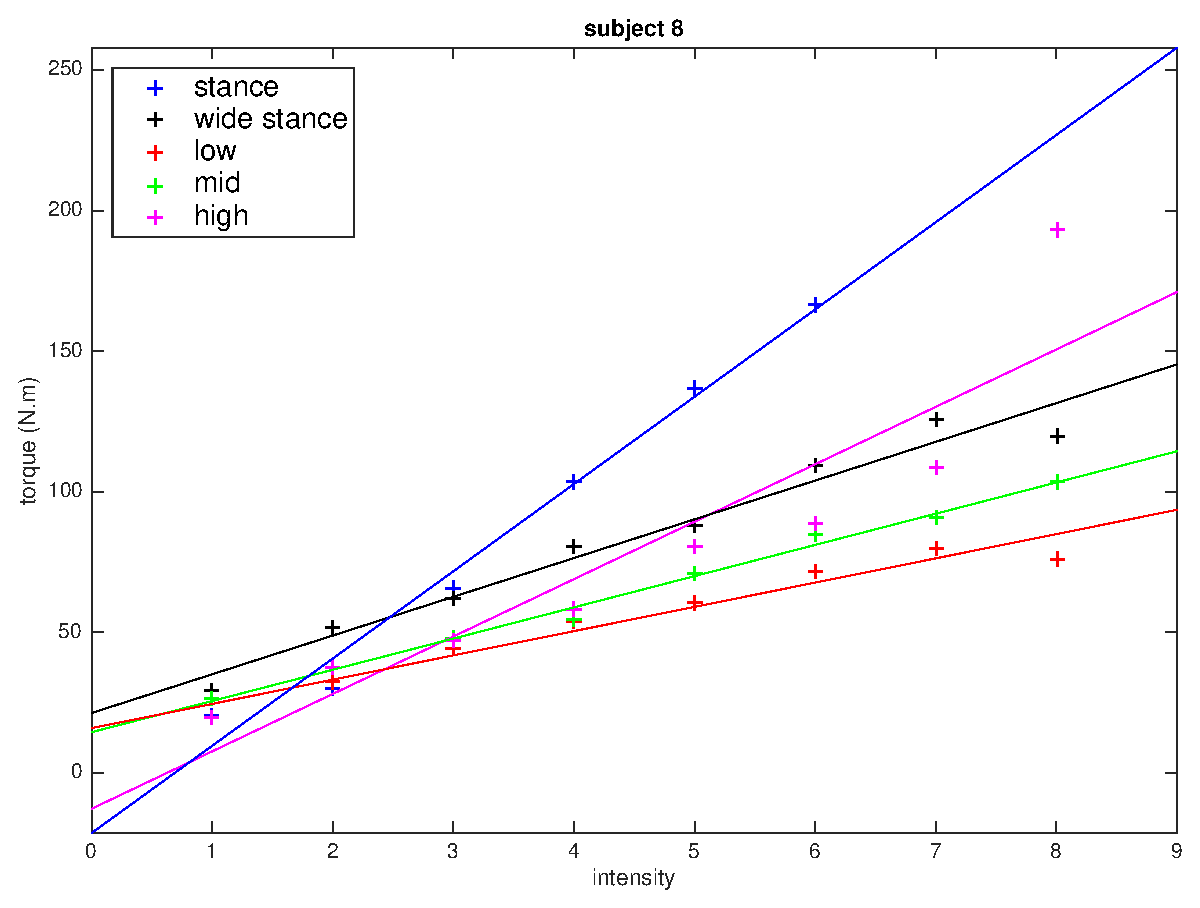
\includegraphics[width=0.46\linewidth]{subj8} \\
%%     subject 9 & subject 10 \\
%%     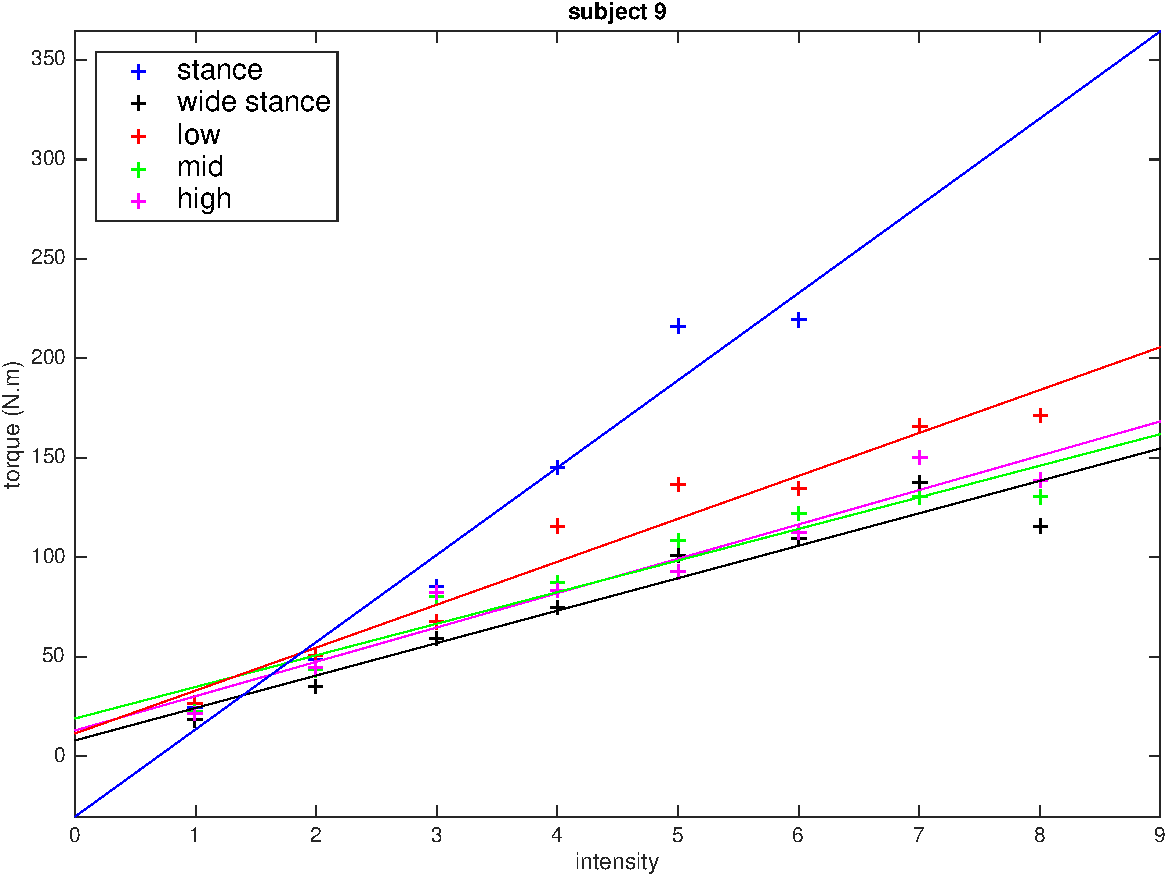
\includegraphics[width=0.46\linewidth]{subj9} &
%%     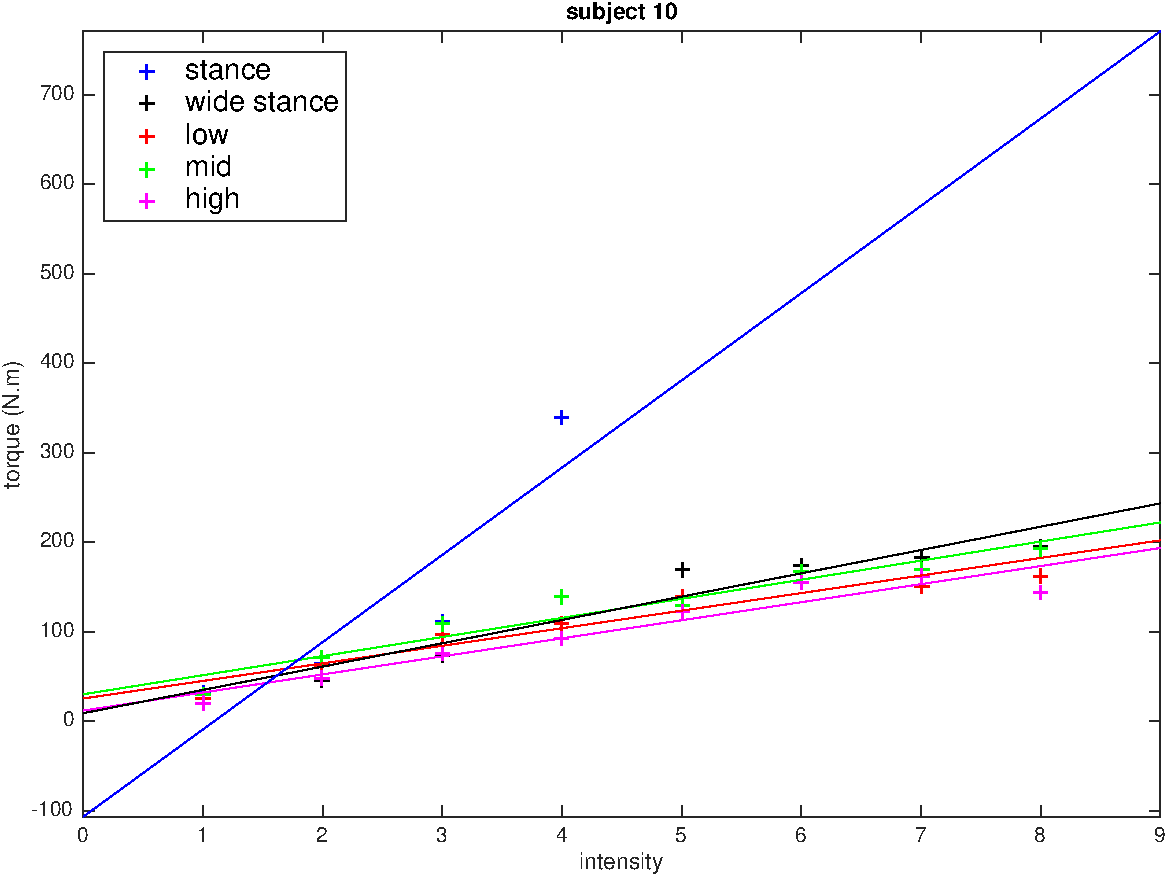
\includegraphics[width=0.46\linewidth]{subj10} \\
%%   \end{tabular}
%%   \caption{Total average normalized joint torques for the subjects at
%%     different perturbation magnitudes and different poses: stance (blue), low
%%     handle (red), middle handle (green) and high handle (magenta).}
%%   \label{jointtorquesubjects}
%% \end{figure}

The means of the normalized joint torques (per subjects) is shown in Fig.~\ref{jointtorque}. This figure shows the total average torque (after removing outliers) for all subjects at each configuration and each intensity. The lines are fitted to the values by using least squares method. The standard error of the means are also shown in this figure. As can be seen in this figure, the low handle pose has the lowest total torque and the stance pose has the highest. According to this graph, the ranking between the positions is 1) low, 2) middle, 3) high, 4) wide stance and 5) stance. This ranking is more visible in higher intensities and it conforms with the manipulability numbers from our analysis. The only difference is that manipulability analysis predicts that middle and high positions are the same whereas experimental results show a bit difference between two (middle is better than high). Therefore, the experimental results agree with the manipulability analysis in the previous subsection. Configurations of greater manipulability require less torque, in order to maintain balance after perturbations of equivalent magnitudes.
\begin{figure}
	\centering 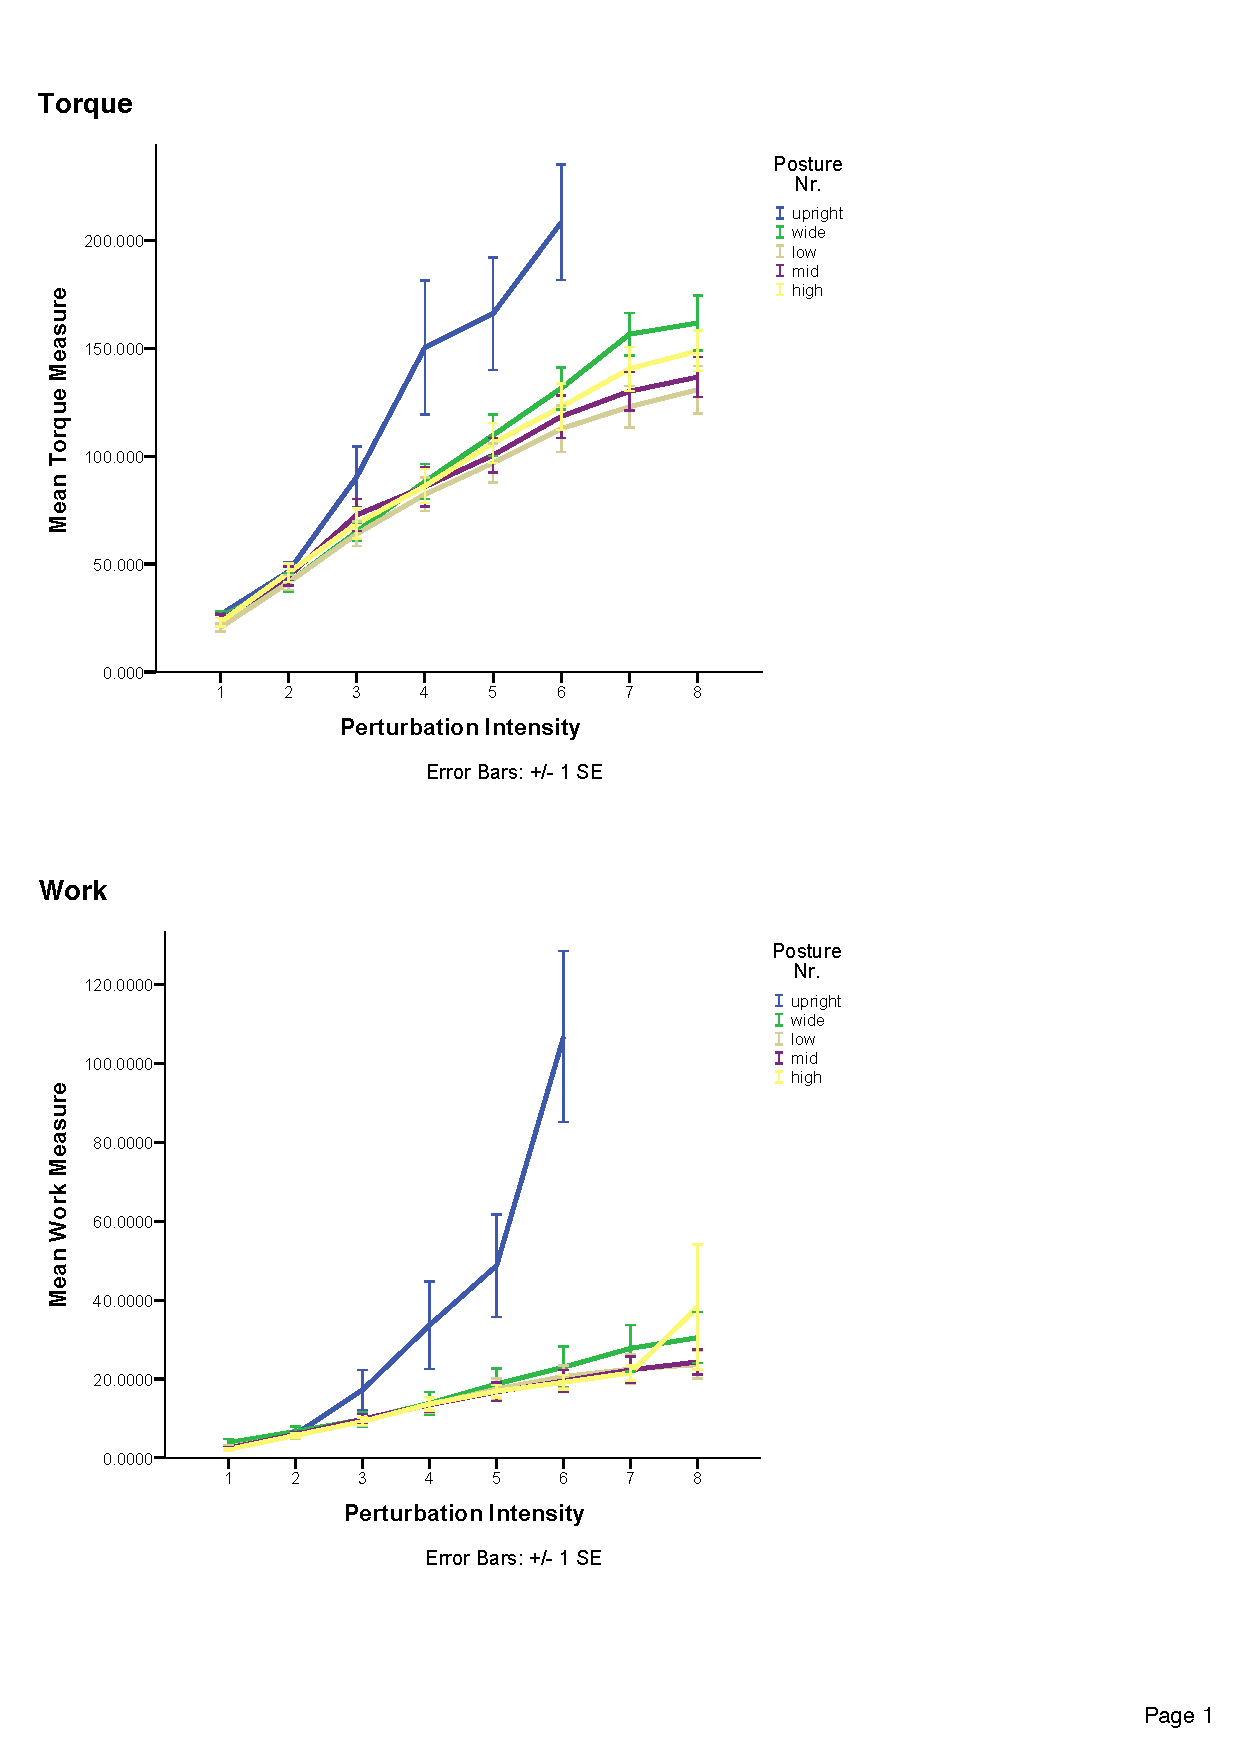
\includegraphics[trim = 1mm 150mm 10mm 10mm, clip, scale =
	0.95]{errorBarPlotsSEM-norm_v2}
	\caption{Average of the total torque for the subjects at each pose and each perturbation intensity. The stance position required the most torque in order to maintain balance. While the low handle position required the least amount of torque for the same perturbation.}
	\label{jointtorque}
\end{figure}


\textbf{Conclusion:} A set of metrics are introduced in this chapter to study, analyse and measure the ability to balance for humans and robots. These metrics, which are called the manipulability of the center of mass, provide two types of ellipsoids which graphically show how the CoM can be accelerated in 3D space by a certain amount of change of motion (due to impulses) at the joint space. These ellipsoids can be used to measure torque efficiency and maneuverability of humans and robots. The proposed metrics are applicable to floating base robots with non-breakable contacts with the environment. Also, experiments on human subjects are performed to investigate the applicability of the proposed metrics for human studies. In the experiments, the standing subjects (in five different configurations) were perturbed by a controlled force acting on their CoM. Then, the selected configurations were ranked according to the average total torque that is applied by the subjects to recover their balance at each configuration. It is shown that the proposed metric for torque efficiency can successfully predict the same ranking between the configurations as the experimental results suggested. This agreement shows the applicability of the metrics for human studies as well. Therefore, manipulability of the center of mass provides greater insight into the posture controllability of humans and robots, in various configurations and contact conditions.

%%%%%%%%%%%%%%%%%%%%%%%%%%%%%%%%%%%%%%%%%%%%%%%%%%%%%%%%%%%%%%%%%%%%%%%%%%%%%%%%
\subparagraph{Whole-body human dynamics estimation for compliant human-robot interaction} 
%~\par
Although if not directly scheduled as a task for the third year, IIT is currently involved in the development of a human wearable prototype of sensors suit.  In an interactive scenario where humans and robots will safetly share a common workspace, the proposed suit tracks motions of the human and records the forces that he is exchanging with the robot giving in real-time  and \emph{in situ} a whole-body estimation of the dynamics of the human itself.  This novel technology will endow robots with the ability to understand and control physical collaboration in a human interaction.

\textbf{Introduction and problem statement:} Human whole-body motion tracking is nowadays a well-established tool in the analysis of human movements. Well known examples include: a wearable marker-less technology suitable for outdoor motion capturing produced by Xsens \cite{roetenberg2009xsens}, a state-of-the-art marker-based technology for in lab applications produced by Vicon, and Microsoft's Kinect depth camera system which allows marker-less low-cost whole-body motion tracking for  indoor applications \cite{zhang2012microsoft}.
Although existing technologies provide a high level of accuracy in computing motion quantities, they have several limitations in measuring kinetic quantities in real-time (kinetics considers forces that cause movements).  A key problem lies in the fact that motion capture methods typically employ only kinematic measurement modalities (position, velocities and accelerations) \cite{Bonnet2013} and does not include information on the kinetics of human movements.  
Whole-body force tracking is not a new challenge for the scientific community but the topic has been seldom explored \emph{in situ} due to the computational difficulties of the analysis and even more rarely analyzed in a real-time modality. Although several recent studies are going in this direction, it is limited to prototypical and non-wearable technologies. 

\textbf{ Methodology:} Our methodology attempts to estimate dynamics quantities by exploiting the fusion of the sensor information on a probabilistic Gaussian framework in presence of redundant (and noisy) measurements \cite{Latella2015}.  The framework is based on the idea of building a joint probability for all the dynamic variables and measurements coming from multiple sensors and to compute the estimation as the conditioned probability of the variables themselves given the measurements.  Preliminary results show that the variance associated to each estimated variable decreases as the number of considered measurements (sensors) increase.
% TODO:
%	Add PMs from UB
%	Get agreement from TUD, UPMC

%!TEX root = ../../secondYearReport.tex
\subparagraph{Resources}
Overall, the use of resources within WP2 was in accordance to the plans. There was an increase in the amount of PM for JSI due to the fact that we could not find a suitable Post-doc but hired a PhD student instead. Consequently we foresee approximately 25\% increase in total amount of PM at the end of the project.

\begin{center}
\begin{tabular}{|C{1.5cm}|C{1.5cm}|C{1.5cm}|C{2cm}|C{2cm}|C{2cm}|C{2cm}|}
\hline
\footnotesize \textbf{WP2 person months}& \footnotesize \textbf{IIT}&\footnotesize \textbf{TUD}&\footnotesize \textbf{UPMC}& \footnotesize \textbf{UB} &\footnotesize \textbf{JSI} & \footnotesize \textbf{INRIA} \\ \hline
\footnotesize Year 1 &  0.00     & 0.00 & 0.28 & 2.64 & 18.80  &-  \\  \hline
\footnotesize Year 2 &  0.00     & 3.00 & 0.48 & 7.67 & 21.85  &-  \\  \hline
\footnotesize Year 3 &  0.00     & 1.00 & 1.20 & NaN & 21.69  & 0.50  \\  \hline
\footnotesize Partial &  0.00     & 4.00 & 1.96 & NaN & 62.34 & 0.50 \\ \hline \hline
\footnotesize Overall & 0.00     & 4.00 & 1.00 & 45.00 & 55.00 & 1.00 \\ \hline
\end{tabular}
\end{center}

\subparagraph{Deviations from workplan} 
No significant deviations.

%!TEX root = ../../fourthYearReport.tex


 
\paragraph{Work package 3 progress}

The progress for each task are described hereafter.

\subparagraph{Solving the local control problem (T3.3) (UPMC: 1PM, IIT: xxPM)}

\begin{itemize}
\item {Joint limit avoidance using an exogenous state description}
\end{itemize}
During year 4, IIT proposed a control laws ensuring the stabilization of a time-varying desired joint trajectory and joint limit avoidance (see Fig.~\ref{fig:icub leg limits} for an illustration of the limits on the leg) in the case of fully-actuated manipulators. The key idea is to perform a parametrization of the feasible joint motion space in terms of exogenous states $\xi$, in the form of $q(\xi) := \delta \tanh(\xi) + q_0$, where $q$ is the joint position, $\delta$ the range of feasible motion and $q_0$ its middle value. It follows that the control of the exogenous states allows for joint limit avoidance. One of the main outcomes of this work is that position terms in control laws are replaced by parametrized terms. Stability and convergence of time-varying reference trajectories obtained with the proposed method were demonstrated to be in the sense of Lyapunov. The introduced control laws were verified by carrying out experiments on two degrees-of-freedom of the torque-controlled iCub. This work led to a publication in Humanoid s 2016 \cite{charbonneau2016Humanoids}.

\begin{figure*}
   \begin{center}
    \includegraphics[width=0.4\textwidth]{images/iCub_joint_limits_leg.pdf}
    \caption{iCub leg setup used for the experiments. The red circles identify the hip and knee joints, while the white marks indicate joint limits. The green arrow shows the external force applied during experiments.}
    \label{fig:icub leg limits}
    \end{center}
\end{figure*}


\begin{itemize}
\item {Whole-body controller implementation}
\end{itemize}
As part of both WP1 and WP3, UPMC has pursued the generic implementation of an optimisation based whole-body controller named OCRA. See section~\ref{sec:OCRA}) for more details and \url{https://github.com/ocra-recipes} and \url{https://ocra-recipes.github.io/web} for online resources.

\subparagraph{Bootstrapping and validating the control approach in rigid world and compliant cases (T3.4) (JSI: 1 PM, INRIA: 1.98PM , TUD: 3.6 PM)}

\begin{itemize}
\item \textbf{Learning torque control}
\end{itemize}
TUD and INRIA, in collaboration with WP4, continued the collaboration on the topic of learning torque control in presence of multiple contacts, exploiting the force/torque and tactile sensors of iCub. Machine learning techniques were used to directly learn the mapping from both skin and the joint state to torques, using mixtures of contact models. Recently, the model was improved for torque control by addressing critical issues in learning from high-dimensional inputs, such as the artificial skin. It was demonstrated that it is possible to considerably reduce the dimensionality of the skin data preserving the information content of the contact position by using stacked auto encoders. A journal paper is currently in preparation. This technique will allow improving torque control in presence of multiple contacts (rigid and/or soft). This work is part of the PhD thesis work of Roberto Calandra on ``Bayesian Modeling for Optimization and Control in Robotics'' \cite{calandra2016PhD}.\\

\begin{itemize}
\item \textbf{Learning soft priorities}
\end{itemize}
INRIA also designed a multi-task prioritized controller with soft task priorities. The controller was first designed in \cite{Modugno2016} and applied to classical manipulators. In \cite{modugno2016learning} it was extended for whole-body movements. In the latter work, it was used to generate safe whole-body behaviors for iCub, reaching multiple goals and avoiding obstacles, with the guarantee that the generated behaviors were not violating the constraints of the platform. A software controller for iCub has been prototyped in Matlab then in C++.

\begin{itemize}
\item \textbf{Task compatibility optimization}
\end{itemize}
As part of both WP4 and WP3, UPMC has worked on improving its approach for task compatibility optimization. Modern control architectures employ multiple levels of control in order to decouple complex behaviors into manageable control problems. At the lowest level is reactive whole-body control, where joints torques are calculated at high frequency ($\sim1$kHz) given one or more tasks \cite{Khatib2004}. As presented in Deliverable~3.2~\cite{deliverable32}, the control problem can be written as a constrained convex optimization, where the objective function is a combination of task errors, and the constraints are the equations of motion, articulation and actuation limits, and contacts \cite{Salini2011, Saab2013, Bouyarmane2011}. Task errors are calculated as the difference between the current task state and its reference value. This reference value comes from the next level of task servoing. At this level, closed loop controllers are used to servo task trajectories using state feedback (PID) or Model Predictive Control (MPC) schemes at frequencies between $100$Hz and $10$Hz  \cite{Ibanez2014}, \cite{Koenemann2015}, \cite{Perrin2015}. These task trajectories are provided by higher-level open-loop planning which takes seconds to minutes, and generally combines operator expertise and automated planning algorithms \cite{Bouyarmane2012, Pham2014}. This control hierarchy of planning, servoing, and whole-body control is presented in Fig.~\ref{fig:control_diagram}.\\

Because each level in the control hierarchy is agnostic of the others by design, there is no guarantee that the planned task trajectories will be executed properly by the lower control layers~\cite{padois-HDR2016,ibanez_humanoidhandbook2016}. Furthermore, even though specific contexts such as non rigid contacts may be accounted for as described in Deliverable~3.2~\cite{deliverable32}, tasks may conflict with one another or be infeasible with the system constraints \cite{Bouyarmane2015, Wieber2017}. The end result is typically unstable or undesirable whole-body behaviors, and these tasks can be qualified as \textit{incompatible}. Prioritization techniques presented in Deliverable~3.2~\cite{deliverable32} use weighted sums\cite{Salini2011, Bouyarmane2011}, hierarchies~\cite{Saab2013,Escande2014, Dietrich2015} or a mix of both~\cite{liu-AutRob2015,liu-AutRobSI2015} to manage task incompatibilities at the whole-body control level, but are difficult to tune and only hide the problem. Moreover, tasks incompatibilities may be temporal and change over the course of the movement so applying static priorities may be overly restrictive. While the works presented in Deliverable~4.3~\cite{deliverable43} provide very powerful tools to reactively adapt priorities~\cite{Lober2015}, learn proper prioritizations~\cite{Modugno2016,modugno2016learning} or derive them from demonstrations~\cite{Paraschos_2017}, it seems obvious that well designed tasks should not need to be prioritized.\\

 Given that it is the task reference values which generate the incompatible control optima, an alternative to prioritization tuning is to modify the task trajectories supplied by planning and make them compatible as initially suggested in~\cite{Lober2014}. To do so, a feedback loop must be implemented, which measures the errors induced by incompatibilities and changes the task trajectories to reduce them. It should also take into account the servoing and whole-body control levels with all of their parameters, as well as the robot's dynamics and environment. Given the complexity of the proposed feedback loop, one solution is to use model-free Reinforcement Learning (RL) techniques to modify the trajectories through trial and error by minimizing some cost function using Black-Box Optimization (BBO) solvers \cite{Kober2013}.\\

\begin{figure}[!h]
\centering
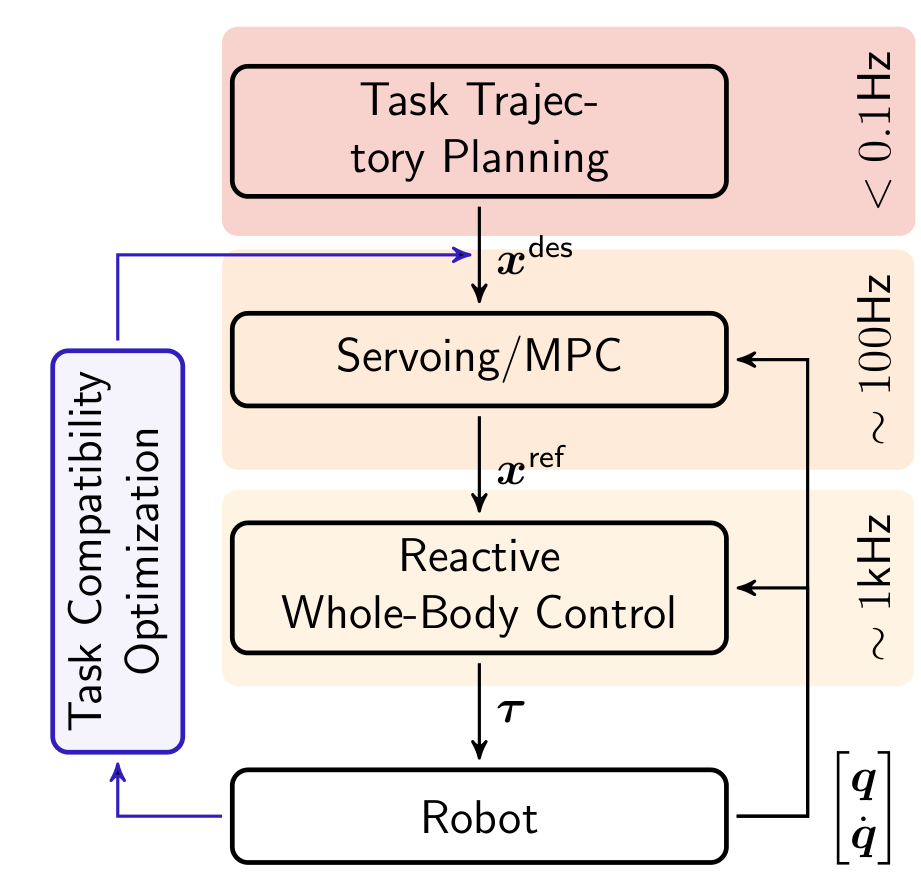
\includegraphics[width=0.4\textwidth]{images/control_pyramid.png}
\caption{A modern control hierarchy for highly redundant robotic systems, e.g. humanoid robots. At the lowest level is whole-body control, which determines the torques needed to accomplish a set of tasks. At the intermediate level, these tasks are controlled by the servoing/MPC level where task trajectory errors are compensated using state feedback. Finally the task trajectories are provided by high-level planning, which is usually a combination of operator expertise and automated planning. Each of these levels operates independently from one another and a feedback mechanism is needed to measure and compensate for tasks which are not executed as planned. This is the role of the Task Compatibility Optimization loop proposed in this work.}
\label{fig:control_diagram}
\end{figure}

The objective of the proposed approach is to establish the task compatibility optimization loop, shown on the left in Fig.~\ref{fig:control_diagram}, by iteratively improving task trajectories using RL. To do so, tasks trajectories are parameterized providing variables with which they can be modified. A generic task compatibility cost has been developed from simple principles which measures the incompatibility between one or more tasks and the robot's constraints. Using two common BBO solvers, this compatibility cost can be minimized by optimizing the task trajectory parameters. This task compatibility optimization has then tested on two typical muti-task scenarios. In the first scenario the relatively banal chore of reaching while balancing has be studied. While seemingly simple, reaching is a key ingredient in robot autonomy, which often requires parameter and gain tuning before done reliably. A performance comparison of two BBO solvers for this experiment has been performed to illustrate the generality of the framework. The second experiment explores the dynamically complex activity of moving from sitting to standing. This motion requires contact breaking and potentially unstable dynamic equilibrium to succeed. In both experiments a Center of Mass (CoM) task is used to maintain balance, and its trajectory is optimized to minimize the task compatibility cost. Through these two completely different motion scenarios, the proposed generic task compatibility optimization loop has shown to dramatically improve task achievement, without ever touching the low-level control parameters. These results extend the contributions \cite{lober-HUMANOIDS2014} and \cite{lober_IROS2015} both in terms of achieved performances and computational efficiency. This work is described in \cite{deliverable33} and was submitted for presentation at a robotics journal~\cite{lober2017RAL-IROS}.

\begin{itemize}
\item \textbf{Speed-Accuracy trade-off}
\end{itemize}
As part of both WP2 and WP3, JSI, together with UPMC, continued the computational study where they try to describe the trade-off between the speed of motion, its accuracy and the muscular cost associated with the motion. They implemented a state-of-the-art deep reinforcement learning algorithm (DDPG) that is based on a deterministic policy gradient approach. DDPG allows more sample efficient learning, but is hard to tune in the context of a simulated reaching controller. They implemented the computations on the JSI cluster in Slovenia. Computations are currently running and the analyses remain to be performed.
    
\subparagraph{Deviations from workplan}  

The PM expenses for WP3 after one year of project are globally conform to the planned one. The observed deviations are related to the fact that tasks 3.3 and 3.4 spans the overall duration of the project and the contribution of some of the partners are expected in the 2nd, 3rd and 4th year.

%\emph{\color{red}[For work package 3 (UPMC) provide the following information:]}
%\begin{itemize}
%\item[-] \emph{\color{red}[A summary of progress towards objectives and details for each task;]}
%\item[-] \emph{\color{red}[Highlight clearly significant results;]}
%\item[-] \emph{\color{red}[If applicable, explain the reasons for deviations from Annex I and their impact on other tasks as well as on available resources and planning;]}
%\item[-] \emph{\color{red}[If applicable, explain the reasons for failing to achieve critical objectives and/or not being on schedule and explain the impact on other tasks as well as on available resources and planning (the explanations should be consistent with the declaration by the project coordinator) ;]}
%\item[-] \emph{\color{red}[a statement on the use of resources, in particular highlighting and explaining deviations between actual and planned  person-months per work package and per beneficiary in Annex 1 (Description of Work);]}
%\item[-] \emph{\color{red}[If applicable, propose corrective actions.]}
%\end{itemize}





%!TEX root = ../../thirdYearReport.tex

\subparagraph{Resources}

\begin{center}
\begin{tabular}{|C{1.5cm}|C{1.5cm}|C{1.5cm}|C{2cm}|C{2cm}|C{2cm}|C{2cm}|}
\hline
\footnotesize \textbf{WP3 person months} & \footnotesize \textbf{IIT}&\footnotesize \textbf{TUD}&\footnotesize \textbf{UPMC}& \footnotesize \textbf{UB} &\footnotesize \textbf{JSI} &\footnotesize \textbf{INRIA} \\ \hline
\footnotesize Year 1 &  9.90 & 4.60 & 15.15 & - & - &  -   \\  \hline
\footnotesize Year 2 &  - & 10.5 & 14.67 & 1.85 & 1.00 &  4.00  \\  \hline
\footnotesize Year 3 &  9.90 & 24.75 & 38.61 & 3.21 & 3.00 & 8.17\\  
% \footnotesize Partial &  9.90 & 24.75 & 38.61 & 1.85 & 3.00 & 4.00 \\ 
\hline \hline
\footnotesize Overall &  9.00 & 24.00 & 43.5 & 10.00 & 4.00 & 10.50 \\ \hline
\end{tabular}
\end{center}

In order to best use the whole-body controllers developed within the framework of WP3, TUD hired a student for setting up the iCub hardware and simulation environment.

\subparagraph{Deviations from workplan}

Due to the resignation of Mingxing Liu from her postdoc position in November 2015, UPMC could not dedicate as many person.months as expected on WP3, in particular T3.4. To compensate for that, UPMC dedicated internal resources on T3.4 (PhD work of Ryan Lober). Also, the recruitment of Jorhabib Eljaik as a postdoc, starting in May 2016, will permit to execute the corresponding work on Model Predictive Control for supportive hand reactive planning over the fourth year. 





%!TEX root = ../../secondYearReport.tex


\paragraph{Work package 4 progress}

\subparagraph{Generalizing and Improving Elementary Tasks with Contacts (T4.3)}

In this task, we aim to generate new skills from data, where elementary skills 
are acquired by imitation learning and transferred to novel situations using 
dynamic systems. During year one, TUD developed a novel representation of 
movement primitives that can be used for imitation learning from noisy observations.
Uncertainty of observed trajectories is explicitely modeled and used to generate new skills.
This movement representation has state-of-the-art capabilities in generalization, 
coupling between the degrees of freedom of the robot, and moreover, 
a time varying feedback controller can be derived in closed form. 
These features are partially illustrated in Figure \ref{fig:promps}.
This work was published
last year at the highly competitive conference on neural information processing \cite{Paraschos_NIPS_2013}.


In another work, published at the international conference on humanoid robots (HUMANOIDS), 
TUD demonstrated that this probabilistic approach for trajectory generation
has superior performance against deterministic policies. The use of
probability distributions over the trajectories increased significantly
 the generalization properties, which was evaluated on a high dimensional table
tennis scenario [Paraschos, A. and  Neumann, G and  Peters, J., 2013]. 
In the future work, we plan to incorporate external torque signals to initiate, 
maintain, and terminate contacts.

TUD also investigated how to learn human robot interaction through imitation. We presented a new approach to robot learning that allows anthropomorphic robots to learn a library of interaction skills from demonstration [H Ben Amor, D Vogt, M Ewerton, E Berger, B Jung and J Peters, 2014]. Traditional approaches to modeling interactions assume a pre-specified symbolic representation of the available actions. For example, they model interactions
in terms of commands such as \emph{wait}, \emph{pick-up}, and \emph{place}. Instead of such a top-down approach, we focused on learning responsive behavior in a bottom-up fashion using a trajectory based approach. The key idea behind our approach is that the observation of human-human collaborations can provide rich information specifying how and when to interact
in a particular situation. For example, by observing how two human workmen collaborate on lifting a heavy box, a robot could use machine learning algorithms to extract an
interaction model that specifies the states, movements, and situational responses of the involved parties. In turn, such a model can be used by the robot to assist in a similar lifting task. Our approach is as an extension of imitation learning to multi-agent scenarios, in which the behavior and the mutual interplay between two agents is imitated


We further extended the above approach by introducing \emph{Interaction Primitives} in [Ben Amor, H.; Neumann, G.; Kamthe, S.; Kroemer, O.; Peters, J., 2014]. Interaction primitives build on the framework of dynamic motor primitives (DMPs) by maintaining a distribution over the parameters of the DMP. With this distribution, we can learn the inherent correlations of cooperative activities which allow us to infer the behavior of the partner and to participate in the cooperation. A conceptual overview is sketched in Figure \ref{fig:interaction_primitives}. A learned Interaction Primitive can be used by a robot to (1) predict the human's next action in the current context, (2) identify the optimal response, (3) synchronize the movement with the human partner.

In the meantime, demonstration-based learning of "optimal trajectories" and stable controllers has been addressed by UPMC, in particular in \cite{stulp2013} where a general, flexible, and compact representation of parameterizable skills is proposed. This work generalizes the standard Dynamic Motor Primitive formulation in \cite{ijspeert2013} and proposes a novel DMP formulation for parametrized skills, based on additionally passing task parameters to the DMP function approximator. This generalizes previous approaches, in particular those which train and execute parametrized skills with two separate regressions. Learning the function approximator with one regression in the full space of phase and tasks parameters allows for more compact models, and the flexible use of different function approximator implementations such as LWPR and GPR, as we demonstrated on the Meka and iCub humanoids robots.

%!TEX root = ../../fourthYearReport.tex

\subparagraph*{Resources}

\begin{center}
\begin{tabular}{|C{1.5cm}|C{1.5cm}|C{1.5cm}|C{2cm}|C{2cm}|C{2cm}|C{2cm}|}
\hline
\footnotesize \textbf{WP4 person months}& \footnotesize \textbf{IIT}&\footnotesize \textbf{TUD}&\footnotesize \textbf{UPMC}& \footnotesize \textbf{UB} &\footnotesize \textbf{JSI} &\footnotesize \textbf{INRIA}\\ \hline
\footnotesize Year 1  &  -  & 8.00 & 2.22 & - & - & -     \\  \hline
\footnotesize Year 2  &  6.04  & 21.70 & 1.69 & 2.15 & 3.00 & 2.01     \\  \hline
\footnotesize Year 3  &  9.79 & 12.00 & 0.74 & 1.68 & 3.00 & 3.30 \\  \hline
\footnotesize Year 4  & ?     & ?    & ?    & ?    & ?    & ?    \\   	\hline
\footnotesize Partial & ?     & ?    & ?    & ?    & ?    & ?    \\
\hline \hline
\footnotesize Overall &  30.00 & 38.00 & 9.00 & 12.00 & 10.00 & 9.00 \\ \hline
\end{tabular}
\end{center}

\subparagraph*{Deviations from workplan} 

No deviations.



%!TEX root = ../../fourthYearReport.tex

\paragraph{Work package 5 progress}

The activities in WP5 are divided into four tasks corresponding to the four years project duration. As a result, during the fourth year CoDyCo results concentrate on T5.4. The main result consist in the implementation of the validation scenario consisting of the balancing with the help of a caregiver. The main scientific contribution is described here \cite{latella2016whole}.

\subparagraph{Scenario 4: learning how to stand up with the help of a human caregiver (T5.4)}

The main contributions to T5.4 have been presented in ``Validation scenario 4: learning how to stand up with the help of a human caregiver'' which discusses the technical implementation of the fourth year validation scenario (see \url{https://github.com/robotology-playground/codyco-deliverables/tree/master/D5.4/pdf}). The software developed for the scenario implementation is released with an open-source license and distributed through github (\url{https://github.com/robotology/codyco}).


\textbf{CoM Dynamic Manipulability for the iCub in a Sitting Configuration}


In this calculations, it is assumed that the robot is in a sitting
configuration with joint angles mentioned in Table \ref{jointangles}.
Shoulder pitch angle ($\alpha$) and elbow angle ($\beta$) are the two
variables which are used to maximize the CoM dynamic manipulability in a
desired direction.  The desired direction of the CoM movement in the beginning
of the motion is horizontal.  The maximum joint torques are assumed to be
$40$N.m. for the legs and $20$N.m. for the arms.
%
\begin{table}[h]
  \centering
  \caption{iCub joint angles in a sitting configuration.  Angles are in
    degrees.}
  \begin{tabular}{|c|c||c|c||c|c|}
    \hline hip pitch   & $91$   & shoulder roll & $12$ & torso pitch & $-5$ \\
    \hline hip roll    & $12$   & shoulder yaw  & $80$ & torso roll  & $0$   \\
    \hline hip yaw     & $0$    & wrist pronos  & $0$  & torso yaw   & $0$   \\
    \hline knee        & $-104$ & wrist pitch   & $0$  & neck pitch  & $0$ \\
    \hline ankle pitch & $-12$  & wrist yaw     & $0$  & neck roll   & $0$ \\
    \hline ankle roll  & $0$    &               &      & neck yaw    & $0.5$ \\
    \hline
  \end{tabular}
  \label{jointangles}
\end{table}
%
\begin{figure}
  \centering
  \includegraphics[scale=0.29]{3Dfigure.pdf}
  \caption{CoM dynamic manipulability with respect to arm configuration.}
  \label{3Dfig}
\end{figure}
%


The CoM dynamic manipulability for different arm configurations
(i.e. different $\alpha$ and $\beta$) is shown in Figure \ref{3Dfig}.  The
maximum manipulability is at $\alpha = -29^\circ$ and $\beta = 32^\circ$.
Figures \ref{2Dfig_shoulder} and \ref{2Dfig_elbow} show CoM manipulability
with respect to the shoulder angle and the elbow angle, respectively.  As it
can be seen in these figures, in case the optimum values are not feasible,
best values for the shoulder angle value is between $-20^\circ$ to $-40^\circ$
and for the elbow angle is about $30^\circ$.  Figures \ref{icub_optimum} shows
the iCub's configurations when the arms angles are in their optimum values.
Figrue \ref{icub_suboptimum} shows the iCub's configuration when $\alpha =
-40^\circ$ and $\beta = 32^\circ$.  In this case, the manipulability is
decreased by $\%3$.
%
\begin{figure}
  \centering \includegraphics[scale=0.4]{2DfigureShoulder.pdf}
  \caption{CoM dynamic manipulability with respect to shoulder pitch angle.}
  \label{2Dfig_shoulder}
\end{figure}
%
\begin{figure}
  \centering
  \includegraphics[scale=0.4]{2DfigureElbow.pdf}
  \caption{CoM dynamic manipulability with respect to elbow angle.}
  \label{2Dfig_elbow}
\end{figure}
%
\begin{figure}
  \centering 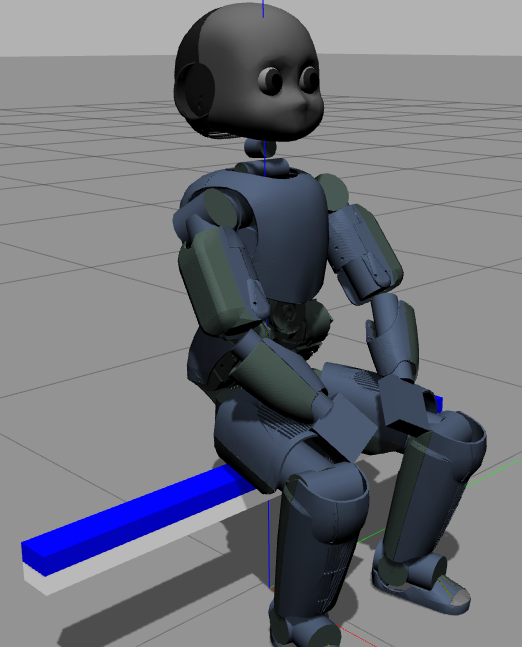
\includegraphics[scale=0.4]{icub_optimum}
  \caption{iCub in optimum sitting configuration.}
  \label{icub_optimum}
\end{figure}
%
\begin{figure}
  \centering
  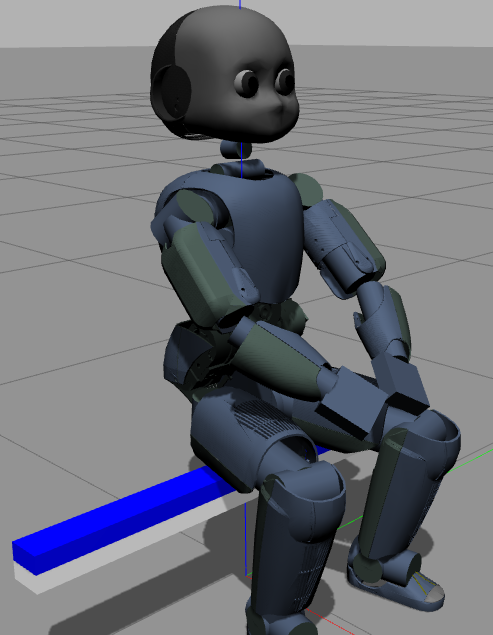
\includegraphics[scale=0.4]{icub_suboptimum}
  \caption{iCub in near-optimum sitting configuration.}
  \label{icub_suboptimum}
\end{figure}
%



\subparagraph{Deviations from workplan}  

No deviations.

%\begin{itemize}
%\item[-] \emph{\color{red}[A summary of progress towards objectives and details for each task;]}
%\item[-] \emph{\color{red}[Highlight clearly significant results;]}
%\item[-] \emph{\color{red}[If applicable, explain the reasons for deviations from Annex I and their impact on other tasks as well as on available resources and planning;]}
%\item[-] \emph{\color{red}[If applicable, explain the reasons for failing to achieve critical objectives and/or not being on schedule and explain the impact on other tasks as well as on available resources and planning (the explanations should be consistent with the declaration by the project coordinator) ;]}
%\item[-] \emph{\color{red}[a statement on the use of resources, in particular highlighting and explaining deviations between actual and planned  person-months per work package and per beneficiary in Annex 1 (Description of Work);]}
%\item[-] \emph{\color{red}[If applicable, propose corrective actions.]}
%\end{itemize}

%!TEX root = ../../fourthYearReport.tex

\subparagraph*{Resources}

Resources were used with no difference with respect to what planned. 

\begin{center}
\begin{tabular}{|C{1.5cm}|C{1.5cm}|C{1.5cm}|C{2cm}|C{2cm}|C{2cm}|C{2cm}|}
\hline
\footnotesize \textbf{WP5 person months}& \footnotesize \textbf{IIT}&\footnotesize \textbf{TUD}&\footnotesize \textbf{UPMC}& \footnotesize \textbf{UB} &\footnotesize \textbf{JSI} & \footnotesize \textbf{INRIA} \\ \hline
\footnotesize Year 1  &  2.00  & -    & 0.31 & -    & - & -     \\  \hline
\footnotesize Year 2  &  12.00 & 0.85 & 0.05 & -    & - & -     \\  \hline
\footnotesize Year 3  &  13.06 & 2.00 & 0.14 & 1.44 & - & 0.52 \\ \hline
\footnotesize Year 4  & ?     & ?    & ?    & ?    & ?    & ?    \\   	\hline
\footnotesize Partial & ?     & ?    & ?    & ?    & ?    & ?    \\
\hline \hline
\footnotesize Overall &  48.00 & 5.00 & 2.50 & - & - & 1.50 \\ \hline
\end{tabular}
\end{center}

\subparagraph*{Deviations from workplan} 
No significant deviations from the workplan. The validation scenarios will include all the theoretical and technological challenges detailed in the original plan.


%!TEX root = ../../thirdYearReport.tex


\paragraph{Work package 6 progress}

Activities within work package 6 achieved the expected results both in terms of administrative activities and management activities. As a major achievement, the management successfully concluded a third amendment to include INRIA as a partner. The inclusion was motivated by the the new position of Dr. Serena Ivaldi, currently researcher at INRIA, Nancy. 

\subparagraph{Administrative coordination (T6.1)}
Administration was successfully coordinated by IIT, with significant contribution from Chiara Andreoli (iCub Facility), Francesca Boscolo (project offices) and Maria Carmela Fierro (Robotics, Brain and Cognitive Science Department). The major activity concerned the amendment that the CoDyCo consortium asked the main reason being the fact that Serena Ivaldi, initially hired by UPMC and successively moved to TUD, was recently hired by INRIA as researcher. Part of the administrative coordination activities were also conducted during the mid-year meeting: November 20th-21st, 2014, Ljubljana.  Details on the meetings can be found in the CoDyCo website (\url{http://www.codyco.eu}).

\subparagraph{Software repository implementation (T6.2)}

The github software repository was several times restructured \url{https://github.com/robotology/codyco} and the contribution from the different developers can be directly checked in the website. 
%!TEX root = ../../thirdYearReport.tex


\subparagraph{Resources}

Resources were used as follows.

\begin{center}
\begin{tabular}{|C{1.5cm}|C{1.5cm}|C{1.5cm}|C{2cm}|C{2cm}|C{2cm}|C{2cm}|}
\hline
\footnotesize \textbf{WP6 person months}& \footnotesize \textbf{IIT}&\footnotesize \textbf{TUD}&\footnotesize \textbf{UPMC}& \footnotesize \textbf{UB} &\footnotesize \textbf{JSI} & \footnotesize \textbf{INRIA} \\ \hline
\footnotesize Year 1 &  1.46 & 0.00 & 0.25 & 0.00 & 0.10 & 0.00    \\  \hline
\footnotesize Year 2 &  1.50 & 0.00 & 0.31 & 0.00 & 0.00 & 0.00     \\  \hline
\footnotesize Year 3 &  NaN & 1.00 & NaN & NaN & 0.44 & NaN     \\  \hline
\footnotesize Partial &  2.96 & 1.00 & 0.56 & 0.00 & 0.54 & 0.00 \\ \hline \hline
\footnotesize Overall &  5.00 & 1.00 & 1.00 & 0.60 & 1.00 & 0.00 \\ \hline
\end{tabular}
\end{center}

\subparagraph{Deviations from workplan} 
No significant deviations. 

%!TEX root = ../../thirdYearReport.tex


\paragraph{Work package 7 progress}

Dissemination and exploitation activities included the participation to international events addressed to both commercial and academic institutions. 

\subparagraph{Dissemination activities towards academia, industry, and other users (T7.1)}

Dissemination activities were conducted thorough international publications, organisation of international events, talks at international conferences, press interviews and iCub expositions at international events. Here is the overall contribution subdivided by partner:

\begin{itemize}

\item IIT: 4 invited talks, 4 organised international events, 6 talks at international conferences, 10 publications (2 journal, 7 internal conferences, 1 book chapter), 10 media coverage events.

\item TUD: 9 invited talks, 1 organised international events, 12 publications (2 journal articles, 10 international conferences), 3 media coverage events, 3 M.Sc. theses and one Ph.D. thesis. 

\item UPMC: 3 invited talks, 6 publications (6 internal conferences), 1 media coverage event.

\item UB: 3 invited talks, 5 publications (5 internal conferences), 5 talks at international conferences.

\item JSI: 1 invited talks, 1 organised special issue, 2 talks at international conferences, 7 publications (1 journal, 6 internal conferences).

\item INRIA: 4 invited talks, 4 organised international events, 8 publications (4 journal, 4 internal conferences), 3 media coverage events

\end{itemize}

Live demonstration of the iCub have been performed at several international events.  Some of these events were sponsored by CoDyCo and the following is a non exhaustive list:

\begin{enumerate}

\item 12$^{th}$-14$^{th}$ March 2014. EU Robotics Forum Rovereto. \url{http://www.erf2014.eu/erf_home.jsp}.
\item 3$^{rd}$-6$^{th}$ June 2014. Automatica 2014, Munich, Germany. \url{http://www.nfm-automatica.de/2014/en/home.php}.
\item 3$^{rd}$-5$^{th}$ October 2014. European Maker Faire, Roma, Italy. \url{http://www.makerfairerome.eu/en/agenda2014/}. 
\item 18$^{th}$-20$^{th}$ November 2014. 2014 IEEE-RAS International Conference on Humanoid Robots (Humanoids 2014), Madrid, Spain. \url{http://www.humanoids2014.com}.

\end{enumerate} 

Among the invitations as a speaker at international events it is worth citing the following:

\begin{enumerate}

\item Francesco Nori: invited speaker at the Journ�es Nationales du GdR Robotique 2014, held at Grand amphith\'e\^atre du Centre Arts et M\`etiers ParisTech, 151-155 boulevard de l'H�pital, 75013 Paris. 30 October 2014. \url{http://www.gdr-rob2014.org}.

\item Serena Ivaldi: invited speaker French-German-Japan Workshop on Humanoid and Legged robots. Social learning and engagement in human-humanoid interactions. \url{http://orb.iwr.uni-heidelberg.de/hlr2014/HLR14}.

\item Jan Babic: invited talk in Paris at the Universit� Pierre et Marie Curie. Synthesis of skilled robotic behaviour through human sensorimotor adaptation:  12$^th$ November 2014.

\item Jan Peters: keynote for the Learning by Demonstration Session Topic at the IEEE/RSJ International Conference on Intelligent Robots and Systems (IROS), Chicago, USA.

\item Jan Peters: invited plenary talk speaker at the 13th International Conference on Intelligent Autonomous Systems (IAS-13), Padua, Italy.

\item Vincent Padois: invited talk at the Cap Digital/Innorobo day about Robotics et Innovations. ``Issues and challenges of interactive robotics in complex industrial contexts''. Lyon, France - March 2014.

\item Michael Mistry: invited Lecturer at European Computational Motor Control Summer School. June 15$^th$-21$^st$, 2014.

\end{enumerate} 

Among the organised international events here is a non exhaustive list of the most relevant events:

\begin{enumerate}

\item IIT: workshop organisation at the 2014 IEEE-RAS international conference on humanoid robots (Humanoids 2014). ?One day with a humanoid robot: a crash course on the iCub software tools?. Coordinators: L. Natale, F.Nori, U. Pattacini, V. Tikhanoff, M. Randazzo, G. Metta (Italy).

\item IIT: iCub summer school (Veni Vidi Vici 2014). In 2014, the school was held in Sestri Levante, Italy, July 21-30 2014. Main organisers: Giorgio Metta, Lorenzo Natale, Francesco  Nori, Vadim Tikhanoff, Ugo Pattacini.

\item INRIA, TUD, UB, JSI: editors for the Autonomous Robots special Issue: ``Whole-body control of contacts and dynamics for humanoid robots''. 

\end{enumerate} 



\subparagraph{Exploitation plan (T7.2)}

The third year activities on T7.1 and T7.2 are all contained in ``D7.1 Dissemination and exploitation plan'' available here: \url{https://github.com/robotology-playground/codyco-deliverables/tree/master/D7.1/pdf}.

\subparagraph{Management of IPR (T7.3)}

No activities to be reported during the third year on this task in consideration of the fact that the task started at the very end of the third year. As a minor starting activity the consortium circulated a list containing each partner responsible contact person for the IPR management. This list is contained in ``D7.1 Dissemination and exploitation plan'' available here: \url{https://github.com/robotology-playground/codyco-deliverables/tree/master/D7.1/pdf}.

\subparagraph{Dissemination of a database of human motion with contacts (T7.4)}

During the third year of CoDyCo, IIT completed the task of setting up a database for storing both human and robot datasets. The details on the database are reported in ``D7.2 Standard database with support materials'' available here \url{https://github.com/robotology-playground/codyco-deliverables/tree/master/D7.2/pdf}. 


%!TEX root = ../../thirdYearReport.tex


\subparagraph*{Resources}

Resources were used as follows.

\begin{center}
\begin{tabular}{|C{1.5cm}|C{1.5cm}|C{1.5cm}|C{2cm}|C{2cm}|C{2cm}|C{2cm}|}
\hline
\footnotesize \textbf{WP7 person months}& \footnotesize \textbf{IIT}&\footnotesize \textbf{TUD}&\footnotesize \textbf{UPMC}& \footnotesize \textbf{UB} &\footnotesize \textbf{JSI} & \footnotesize \textbf{INRIA} \\ \hline
\footnotesize Year 1 &  1.00 & -    & 0.40 & -    & -    & - \\  \hline
\footnotesize Year 2 &  -    & -    & 0.13 & -    & -    & 0.91 \\  \hline
\footnotesize Year 3 &  1.00 & - & 0.64 & - & - & 0.91\\
% \footnotesize Partial & 1.00 & -    & 0.53 & -    & -    & 0.91 \\
\hline \hline
\footnotesize Overall & 3.00 & 1.00 & 1.00 & 1.00 & 1.00 & 1.00 \\ \hline
\end{tabular}
\end{center}

\subparagraph*{Deviations from workplan} 
No significant deviations. 


\subsection{Deliverables and milestones tables}

\subsubsection{Deliverables (excluding the periodic and final reports)}

\begin{figure*}[ht!]
\centering
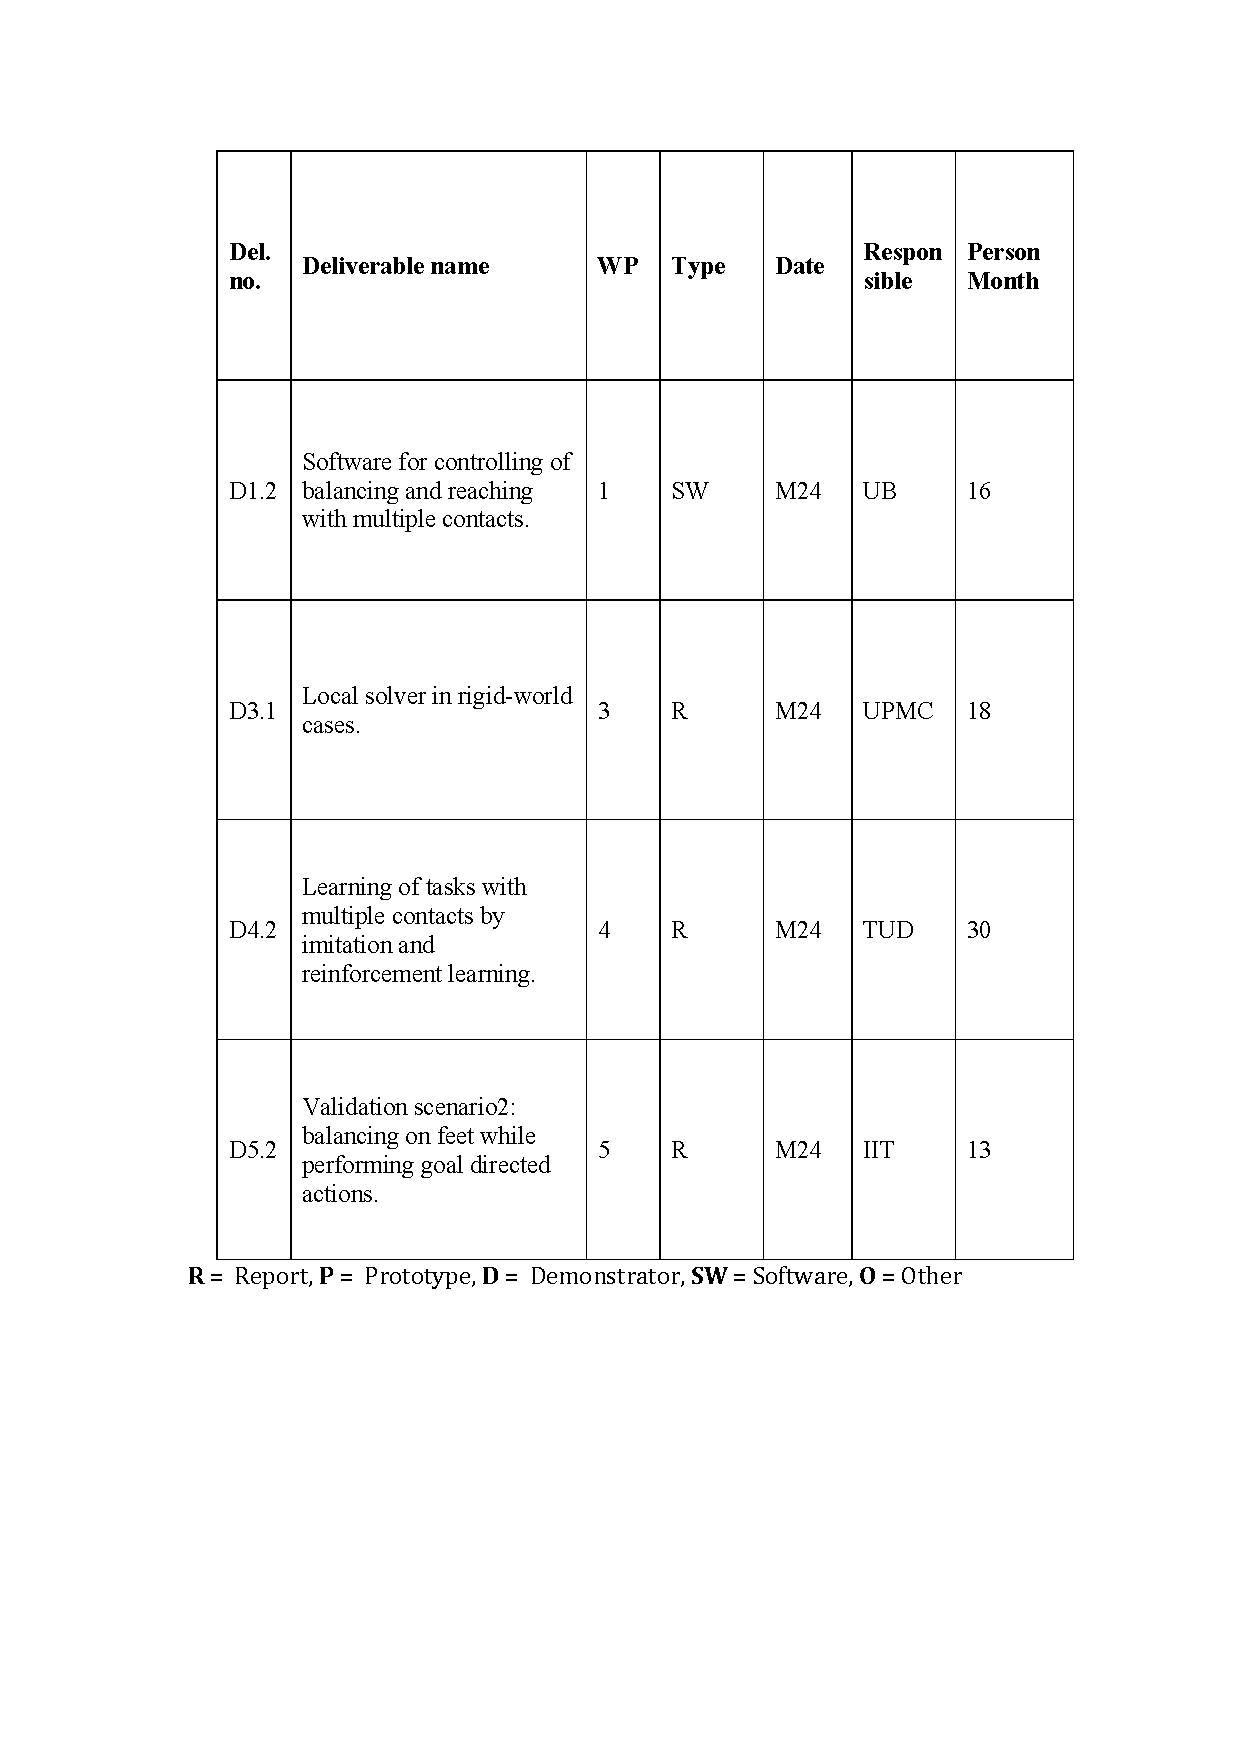
\includegraphics[width=0.6\textwidth]{./images/deliverables.pdf}
\end{figure*}

\subsubsection{Milestones}

\begin{figure*}[ht!]
\centering
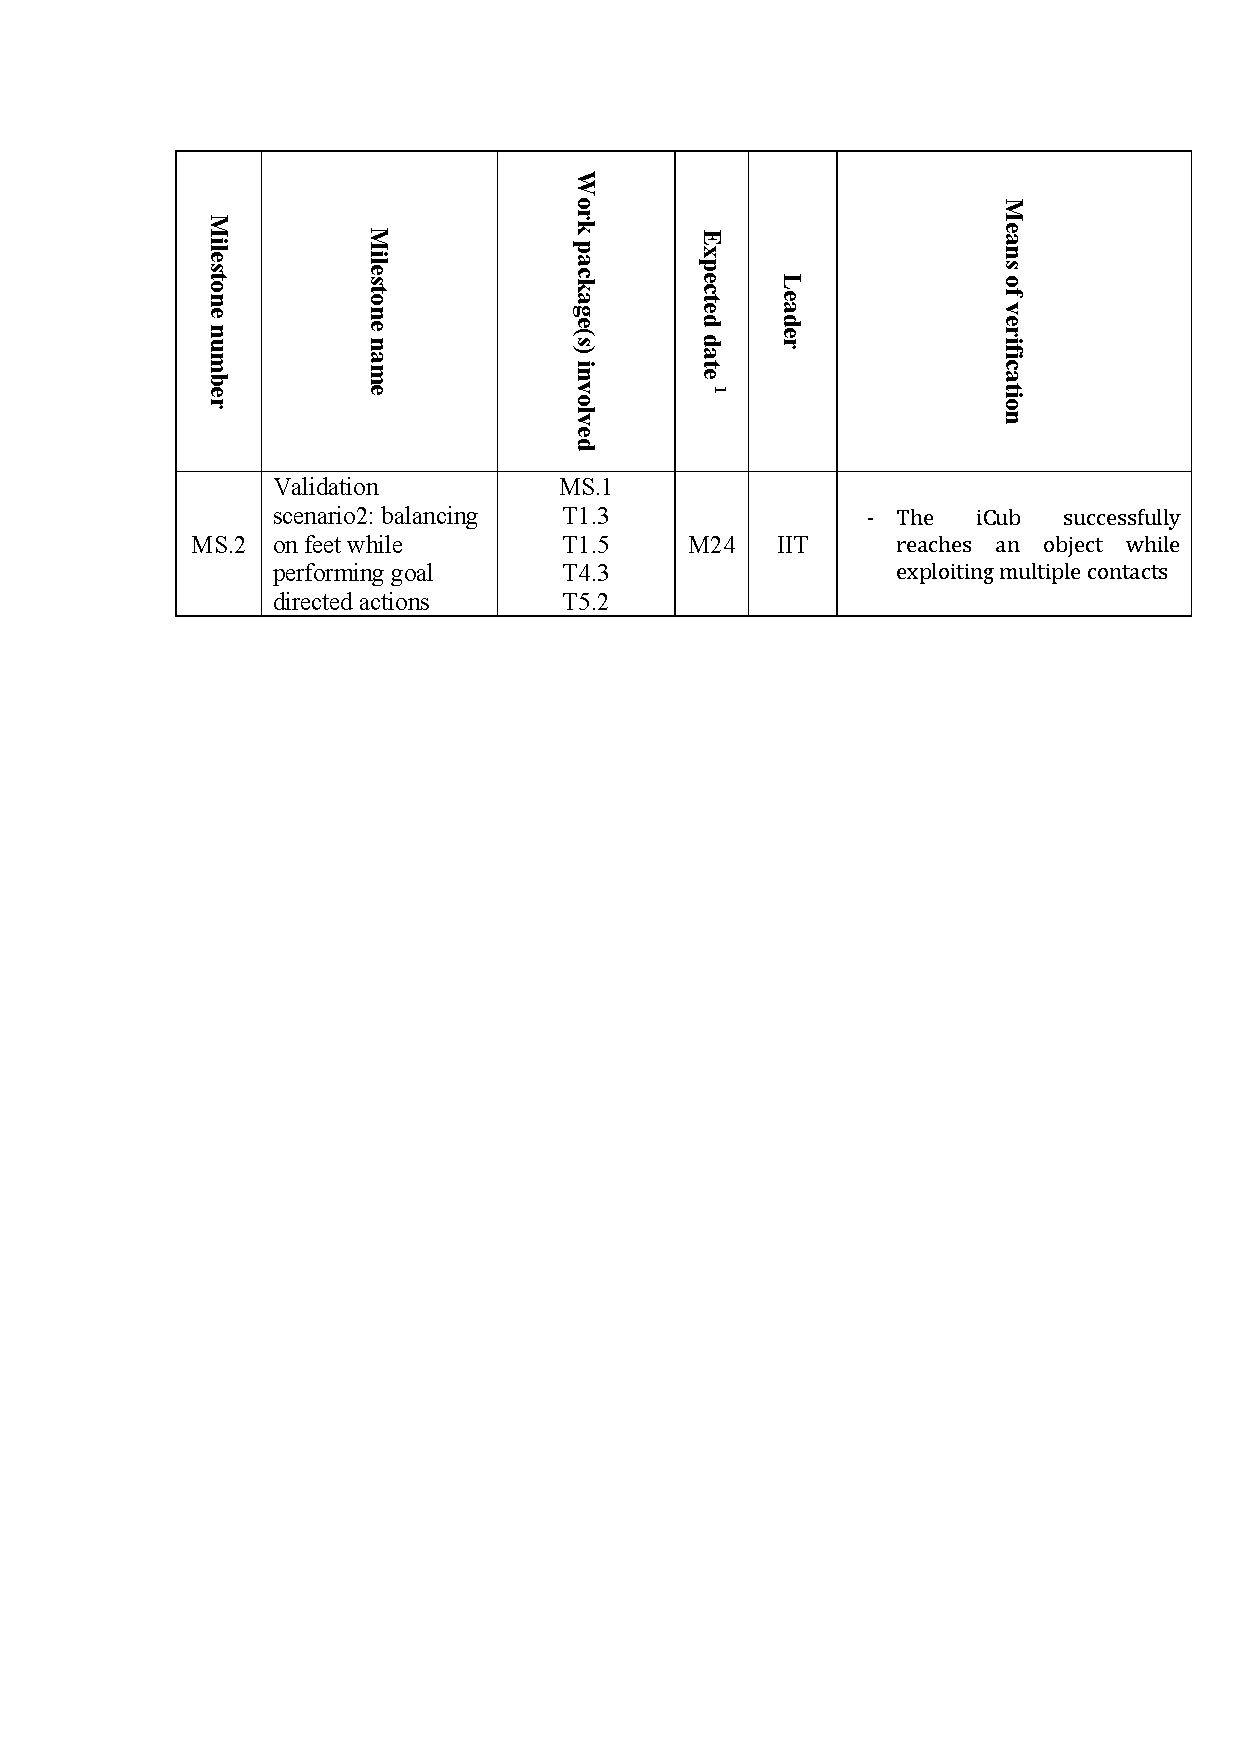
\includegraphics[width=\textwidth]{./images/milestones.pdf}
\end{figure*}

\newpage

\bibliographystyle{IEEEtran}
% \bibliography{IEEEabrv,yearReport_WP3,all-ias-publications}
\bibliography{secondYearReport_WP4,secondYearReport_WP3,secondYearReport_WP2,secondYearReport_WP1}

\end{document}

%%% Local Variables:
%%% mode: latex
%%% TeX-master: t
%%% save-place: t
%%% End:
